\documentclass[12pt]{article}
\usepackage[utf8]{inputenc}
%\usepackage{nips_2017}
\usepackage{graphicx}
\usepackage{natbib}
\usepackage{booktabs}
\usepackage{float}

\usepackage{psfrag}
\usepackage{epsf}
\usepackage{enumerate}

%\bibliographystyle{apalike}

%\bibliographystyle{unsrt} % Use for unsorted references 
\newcommand{\blind}{0}

%\bibliographystyle{plainnat} % use this to have URLs listed in References

% DON'T change margins - should be 1 inch all around.
\addtolength{\oddsidemargin}{-.5in}%
\addtolength{\evensidemargin}{-.5in}%
\addtolength{\textwidth}{1in}%
\addtolength{\textheight}{1.3in}%
\addtolength{\topmargin}{-.8in}%

% Title Page

\bibliographystyle{natbib}

\def\spacingset#1{\renewcommand{\baselinestretch}%
{#1}\small\normalsize} \spacingset{1}

%%%%%%%%%%%%%%%%%%%%%%%%%%%%%%%%%%%%%%%%%%%%%%%%%%%%%%%%%%%%%%%%%%%%%%%%%%%%%%

\begin{document}

\if0\blind
{
  \title{\bf The Effect of Medicaid Expansion on Non-Elderly Adult Uninsurance Rates Among States that did not Expand Medicaid}
  \author{Max Rubinstein \hspace{.2cm}\\
    and \\
    Amelia Haviland \\ \\
    Heinz College, Carnegie Mellon University}
  \maketitle
} \fi

\if1\blind
{
  \bigskip
  \bigskip
  \bigskip
  \begin{center}
    {\LARGE\bf Title}
\end{center}
  \medskip
} \fi

\bigskip

\begin{abstract}

We estimate what the effect of Medicaid expansion would have been on non-elderly adult uninsurance rates in states that did not expand Medicaid in 2014. We estimate this effect by using a synthetic-controls type approach which we adapt for this setting. Previous literature focuses on estimating treatment effects among states that did expand Medicaid. We believe these effects likely differ: existing literature suggests that Medicaid take-up rates are lower among more conservative states. Because Republicans tended to disproportionately govern states that chose not to expand Medicaid, we hypothesize that the effect on uninsurance rates should be smaller in absolute magnitude in non-expansion states compared to expansion states. Using data from the American Communities Survey (ACS), we estimate the effect on non-expansion states by re-weighting expansion regions to approximately balance the covariate distribution from non-expansion regions in an extension of the ``synthetic controls'' framework. We find that Medicaid expansion would have reduced the non-elderly adult uninsurance rate by 2.18 percentage points (1.31, 3.06). These results are indeed smaller in absolute magnitude than existing estimates of the treatment effect on expansion states. We also provide evidence that factors associated with Republican governance may drive this differential.

\end{abstract}

\noindent%
{\it Keywords:} Synthetic controls, balancing weights, treatment effect on the controls, treatment effect on the untreated, overlap weights
\vfill

\newpage
\spacingset{1.45} % DON'T change the spacing!

\maketitle

\section{Introduction}

The 2010 Affordable Care Act required states to expand their Medicaid programs by 2014 to offer coverage to all adults with incomes at least 138 percent of the federal poverty level (FPL). The Supreme Court ruled this requirement unconstitutional in 2012, allowing states to decide whether or not to expand Medicaid coverage. In 2014, twenty-six states and the District of Columbia expanded their Medicaid programs. From 2015 through 2019 an additional ten states elected to expanded their Medicaid programs (\cite{KFF}). This first wave of expansions in 2014 enabled researchers to examine the effects of Medicaid expansion by using expansion states as ``treated'' states, and non-expansion states as ``control'' states. Our goal is to model the effect of 2014 Medicaid expansion on non-elderly adult uninsurance rates among states that did not expand Medicaid. 

We predict that the treatment effect on non-expansion effect will be smaller in absolute magnitude than in states that did expand Medicaid in 2014. Medicaid take-up rates are lower than 100 percent and historically have varied across states (\cite{sommers2012understanding}). This variation is partly a function of state discretion in administering programs: for example, program outreach, citizenship verification policies, and application process differ across states (\cite{courtemanche2017early}). We are especially concerned about how the political composition may drive differences between states. Prior to the 2014 Medicaid expansion, \cite{sommers2012understanding} found that conservative political ideology was associated with lower Medicaid enrollment take-up rates, even after controlling for a variety of correlated policies. Most importantly, political ideology appears to have largely driven a state's decision to expand Medicaid in 2014. Figure \ref{fig1} plots a measure of each state's 2013 institutional ideology by their Medicaid expansion status (\cite{fording}). Higher values of this score correspond to more liberal government institutions. The red dashed line indicates the mean expansion state score and the gray dashed line indicates the mean non-expansion state score. Figure \ref{fig1} illustrates that non-expansion states are more conservative than expansion states.  If these differential take-up rates observed by \cite{sommers2012understanding} continue to hold post-expansion, we should expect treatment effects on non-expansion states to be smaller in absolute magnitude than treatment effects on expansion states. 

\begin{figure}
    \begin{center}
    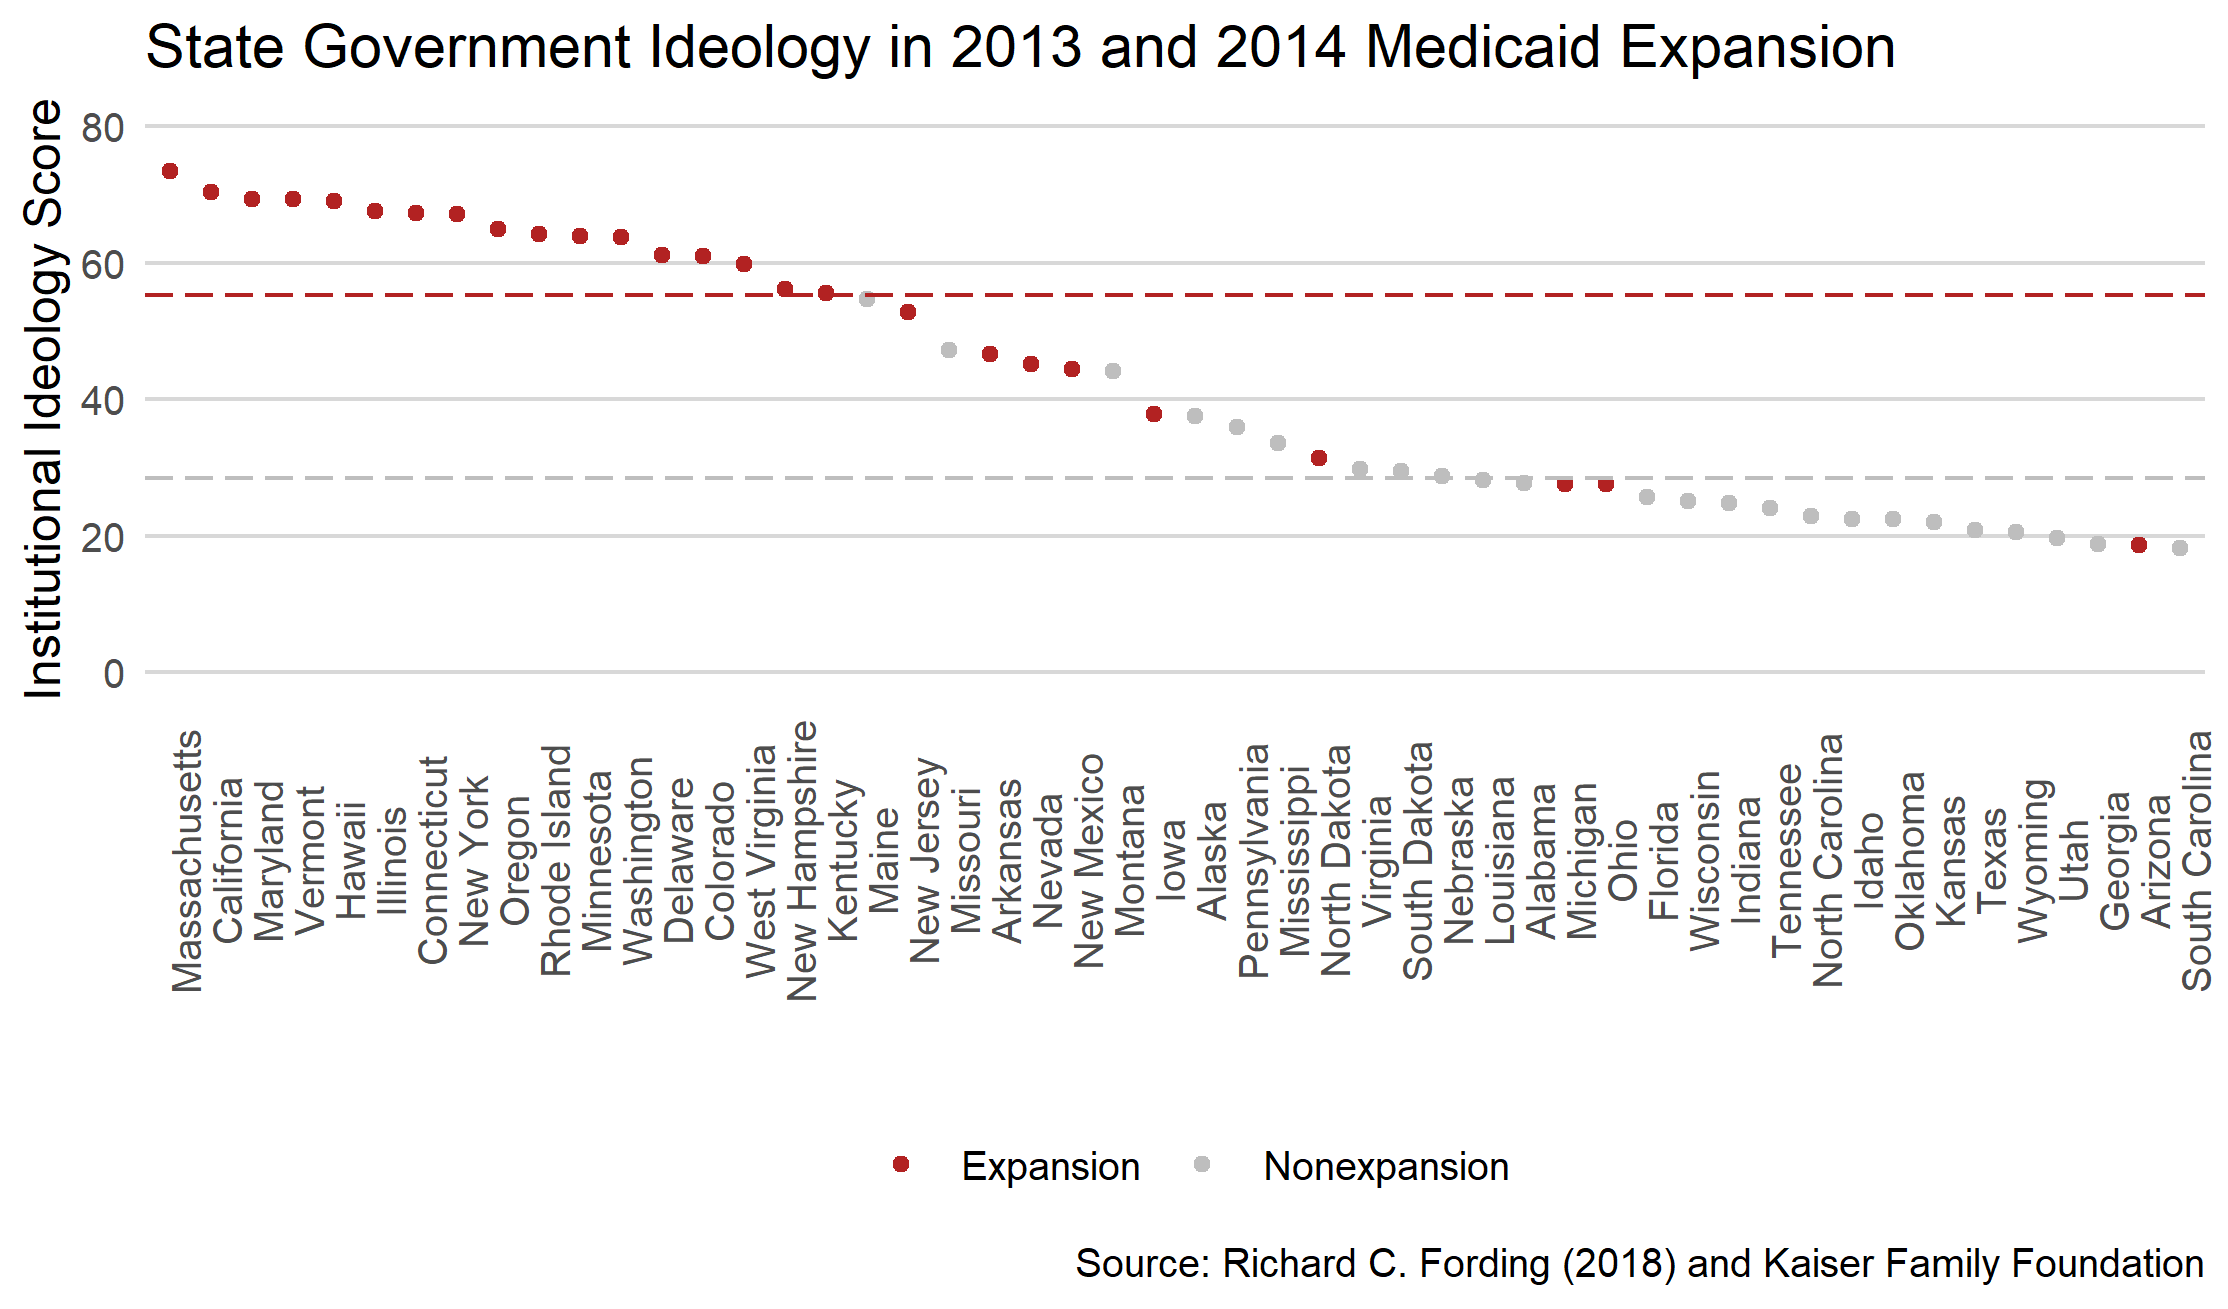
\includegraphics[scale=0.7]{images/political-expansion-plot.png}
    \caption{Government ideology and Medicaid expansion}
    \label{fig1}
    \end{center}
\end{figure}

This paper also has a methodological aim: specifically, we extend the ``synthetic controls'' framework to estimate the ETU and to clarify the required assumptions. While balancing on pre-treatment outcomes alone arguably suffices for some synthetic control applications (see, eg, \cite{botosaru2017role}), here we want to estimate treatment response. We therefore assume no unmeasured confounding given a rich covariate set and a linear and additive outcome model that accounts for all interactions between treatment and the covariates. We then use an implementation of Stable Balancing Weights (\cite{zubizarreta2015stable}) to estimate a set of positive weights to weight the expansion regions to approximately match the covariate distribution of the non-expansion regions. 

We address three additional challenges in our application: limited overlap, bias from sampling variability in our covariates, and variance estimation. As Figure \ref{fig1} suggests, covariate overlap is limited between expansion and non-expansion states, particularly by state political composition. After generating our balancing weights, we therefore use outcome modeling to debias our treatment effect estimates (see, eg, \cite{ben2018augmented}). We then compare these estimates to the overlap average treatment effect (OATE), by overlap weights (proposed by \cite{li2018balancing}), and show that the overlap region is closer to the non-expansion than the expansion region. 

Second, because we measure our covariates from underlying survey data, the imprecision is a form of classical measurement error which may bias our treatment effect estimates. We use the replicate survey weights provided in the ACS data to estimate the covariance matrix associated with this variability and use this information to correct for this bias. This is first study we are aware of that attempts to correct for sampling variability in the covariates when using balancing weights.

Finally, valid variance estimation with aggregate panel-data is a much-studied topic with little consensus (see, eg, \cite{hahn2017synthetic}, \cite{chernozhukov2017exact}). One commonly used approach considers the covariate and outcome values as known population quantities, and the treatment assignment as random (see, eg, \cite{abadie2010synthetic}). Because our region-level covariates and outcomes are estimates from underlying survey data, we take into account this sampling variability and the randomness in the subsequent weighting process, while conditioning on the observed treatment assignment.

The remainder of this paper has the following structure. Section II provides an overview of the data and defines the study period, outcome, covariates, and treatment. Section III discusses our methods, beginning by defining our target estimand, and then outlining our identification, estimation, and inferential procedures. Section IV presents our primary results and sensitivity analyses. Section V provides a brief discussion of the policy relevance of our findings, and Section VI contains a brief concluding summary of the paper. Supplemental materials may be found in the Appendices.

\section{Data}

Our data source is the annual household and person public use microdata files from the American Community Survey (ACS) from 2011 through 2014. The ACS is an annual survey of approximately three million individuals across the United States; the public use files include information on individuals in geographic areas greater than 65,000 people. The smallest geographic unit contained in these data are public-use microdata areas (PUMAs), arbitrary boundaries that nest within state but not within counties or other more commonly used geographic units. One limitation of these data is a 2012 change in the definition of PUMA boundaries; moreover, these new boundaries overlapped with the previous boundaries. As a result, the smallest possible geographic areas that nest both PUMA coding systems are known as consistent PUMAs (CPUMAs). The United States contain 1,075 total CPUMAs, with states ranging from having one CPUMA (South Dakota, Montana, and Idaho) to 123 CPUMAs (New York). The total number of sampled individuals per CPUMA in any year in our study ranged from 531 (representing an area of approximately 96,000 individuals) to 49,046 (representing over 4.5 million individuals). The median sample size for a given CPUMA across the four years of our study is XXX.

\subsection{Study period}

We start our analysis in 2011 following \cite{courtemanche2017early}, who note that several other aspects of the ACA were implemented in 2010 -- including the provision allowing for dependent coverage until age 26, and the elimination of co-payments for preventative care -- likely induced differential shocks across states. We also restrict our post-treatment period to 2014 only: several additional states expanded Medicaid in 2015, including Indiana, Michigan, and Pennsylvania. However, these states did not expand Medicaid contemporaneously with the 2014 ACA provisions. Without additional assumptions, this second-year expansion therefore represents a different causal estimand. 

\subsection{Covariates}

We use the underlying individual-level ACS survey data and accompanying survey weights to aggregate the data at the CPUMA level. We choose our covariates to approximately align with those considered in \cite{courtemanche2017early} and that we argue plausibly include all potential confounders in the outcome model. Because we are ultimately interested in calculating rates, these variables include both counts that we use for the numerators and denominators of the corresponding rates. We note that balancing on the counts equivalently balances on the rates (see, eg, \cite{robbins2017framework}, who follow a similar strategy).

The denominator counts include: total non-elderly adult population for each year 2011-2014; total labor force for each year 2011-2013; and the total number of households averaged from 2011-2013. We then calculate the total number of females; total number of whites; total number of people born outside of the United States; total number of citizens; total number with less than high school education, high school degrees, some college, or college graduates or higher; the total number living under 138 percent of the federal poverty line (FPL), between 139 and 299 percent, 300 and 499 percent, and more than 500 percent of the FPL; and the total number aged 19-29, 30-39, 40-49, 50-64. We then average these counts from 2011-2013. We also calculate the total number of households with one or more children among all households (averaged from 2011-2013). For each year from 2011-2013 we calculate the total number of unemployed individuals among the total number in the labor force and the total number of uninsured individuals among the non-elderly adult population. We then use Census data to calculate the approximate percentage of people living within an ``urban'' area for each CPUMA (\cite{census}). Finally, we include three state-level covariates reflecting the partisan composition of each state's government in 2013. Specifically, we include an indicator for having a Republican governor, an indicator for Republican control over the lower legislative chamber, and an indicator for Republican control over both chambers of the legislature and the governorship.\footnote{Nebraska is the only state with a unicameral legislature; moreover, the legislature is technically non-partisan. We nevertheless classified them as having a Republican control of the legislature.} 

\subsection{Outcome}

Our primary outcome of interest $Y$ is the non-elderly adult uninsurance rate in 2014. Let $Y_L$ indicate the total number of uninsured in 2014 and $P_L$ be the total number of non-elderly adults in 2014, and notice that $Y = Y_L/P_L$ (for any collection of CPUMAs). We treat $P_L$ as fixed in our models and as being unaffected by the treatment. Our outcome $Y$ is therefore a function of two components, one of which is affected by treatment and the other which isn't. Our approach to estimating $Y$ first models $Y_L$ and then divides by $P_L$. We discuss this further below.

We might consider take-up rates among the Medicaid-eligible population to be a more natural outcome. However, we choose the non-elderly adult uninsurate rate for two reasons, one theoretic and one practical. First, Medicaid eligibility in the post-period is likely endogenous: Medicaid expansion may affect an individual's income and poverty levels, which define Medicaid eligibility. A second reason is to align our study to compare our results with the existing literature, and this is the outcome that \cite{courtemanche2017early} use. One drawback of using this outcome is that the simultaneous adoption of other ACA provisions in 2014 more clearly affects this rate in a way that a more targeted group might not.

\subsection{Treatment assignment}

While some states expanded Medicaid and other states did not, in reality assigning a binary treatment status simplifies a more complex reality. We note three reasons we should be cautious about this simplification. First, states differed substantially in pre-existing Medicaid coverage policies: with perfect data we might consider Medicaid expansion as a continuous treatment with values proportional to the number of newly eligible individuals. The challenge though is correctly identifying newly eligible individuals in the data (see \cite{frean2017premium}, who attempt to address this). Second, \cite{frean2017premium} note that six states adopted partial limited Medicaid expansions prior to 2014: specifically, California, Connecticut, DC, Minnesota, and New Jersey. \cite{kaestner2017effects} and \cite{courtemanche2017early} also consider Arizona, Colorado, Hawaii, Illinois, Iowa, Maryland, and Oregon to have had early expansions. Lastly, timing is an issue: among the states that expanded Medicaid in 2014, Michigan's expansion did not go into effect until April 2014, while New Hampshire's expansion did not occur until September 2014.

Our primary analysis excludes New York, Vermont, Massachusetts, Delaware, and the District of Columbia from our pool of expansion states, because these states had comparable Medicaid coverage policies prior to 2014 (\cite{kaestner2017effects}). We also exclude New Hampshire because it did not expand Medicaid until September 2014. While Michigan expanded Medicaid in April 2014, we leave this state in our treated pool. We consider the remaining expansion states as ``treated'' and the non-expansion states as ``control'' states. We later consider the sensitivity of our results to these classifications by removing the early expansion states noted by \cite{frean2017premium}. Our primary classification of expansion and non-expansion states is unique among similar studies: \cite{courtemanche2017early} classifies all expansion states as treated, and all non-expansion states as control. \cite{frean2017premium} exclude Massachusetts from expansion states. Lastly, \cite{kaestner2017effects} include Delaware, DC, Massachusetts, New York, and Vermont as control states. Our final dataset contains aggregated counts for all of the above variables for 925 CPUMAs in our non-expansion and our pool of expansion states. 414 CPUMAs were in non-expansion states and 511 CPUMAs were in expansion states.

\section{Methods}
\label{sec:methods}

In this section we formally present our causal estimand, our identification and estimation strategies, and our inferential procedure.

\subsection{Estimand}

We seek to estimate the average effect of 2014 Medicaid expansion would have had on the non-elderly adult uninsurance rate in states that did not expand Medicaid. As noted previously, the 2014 Medicaid expansion occurred simultaneously with the implementation of several other major ACA provisions, including (but not limited to) the creation of the ACA-marketplace exchanges, the individual mandate, health insurance subsidies, and community-rating and guaranteed issue of insurance plans (\cite{courtemanche2017early}). Almost all states broadly implemented these reforms beginning January 2014. Conceptually we think of the other ACA components as a treatment ($V$) separate from Medicaid expansion ($A$).

We begin by modeling the total counts of uninsured non-elderly adults. Let $i$ index a CPUMA, $j$ index the state, $t$ index the time period, and let $Y_{L, ijT}^{A_{L, ijT} = a, V_{ijT} = v}$ be the potential number of uninsured given Medicaid expansion and other ACA-reforms at time $T = 2014$. We consider the case where these potential outcomes are deterministic: that is, given any state of the world $A = a, V = v$, a CPUMA has some fixed potential number of uninsured non-elderly adults. We then wish to estimate the following contrast:

$$
\psi_L = \sum_{i: A_{ij} = 0, V_{ij} = 1} Y_{L, ijT}^{A_{ij} = 1, V_{ij} = 1} - Y_{L, ijT}^{A_{ij} = 0, V_{ij} = 1} 
$$

In other words, we want to estimate the difference in the total number of uninsured non-elderly adults among states that did not expand Medicaid, but did implement other aspects of the ACA. Because all states implemented the ACA marketplace expansion in 2014, contrasts with the corresponding potential outcome absent this expansion are not identified. We simplify notation by  removing this variable in the estimand:

$$
\psi_L = \sum_{i: A_{ij} = 0} Y_{L, ijT}^{A_{ij} = 1} - Y_{L, ijT}^{A_{ij} = 0}
$$

We therefore seek to identify the effect of Medicaid expansion in the context of the simultaneous implementation of the ACA, but do not attempt to separately identify the effects of these separate treatments. Notice that because non-expansion states were subject to an intervention the post-treatment period, in contrast to other panel data settings, we never observe $Y_{L, ijT}^{A_{ij} = 0, V_{ij} = 0}$. Because we assume that interactions between the ACA implementation and Medicaid expansion may vary over time, we do not seek to generalize these results outside of 2014. 

Lastly, we need to transform $\psi_L$, which represents the change in the total counts, to $\psi$, which represents the more interpretable change in the uninsurance rate. We therefore treat the total observed 2014 population in each region as exogenous and fixed and divide our estimates of $\psi_L$ by this number. More precisely, let $P_L = \sum_{i: A_{ij} = 0} p_{ijT}$. Our target estimand is then:

$$
\psi = \psi_L/P_L
$$

This estimand contrasts slightly from those considered in the synthetic controls literature, which also work with aggregated rates or per-capita outcomes, but do not separately consider the numerators and denominators of these terms.

\subsection{Identification}

We make the following causal assumptions: consistency, no unmeasured confounding, no anticipatory treatment effects, and positivity of treatment assignment. Consistency states that the observed factual outcome under a given treatment assignment is equal to the potential outcome under that same treatment assignment ($Y_{L, ijT}^{A = a} = Y_{L, ijT} \mid A_{jt} = a$). In other words, we assume that one regions' treatment assignment didn't affect another regions' observed outcome. This assumption is standard throughout the literature, but is often not realistic. Violations of this assumption are likely in our study: for example, \cite{frean2017premium} find evidence that Medicaid expansion drove previously eligible but uninsured individuals to enroll in Medicaid in both expansion and non-expansion states. Signing the potential bias from these spillovers requires redefining the causal estimand: for example, we might consider the treatment effect on the untreated given that all states have expanded Medicaid, where the contrast is against where only the observed expansion states expanded Medicaid (ie $n_c^{-1}\sum_{i: A_i = 0}(Y_{L, ijT}^{A_1 = ... = A_{n_t} = 1, A_{n_t + 1} = ... = A_{n_t + n_c} = 0} - Y_{L, ijT}^{A_1 = ... = A_{n_t + n_c} = 1}$). If spillovers occurred in equal proportions in each region, and the magnitude of the spillovers increase with the number of treated regions, then the true effect would be larger in absolute magnitude than the effect estimated using the observed data. We could consider other estimands or assumptions to get different predictions about the sign of the bias, but we leave this as an area for future work.

We next assume that there were no anticipatory treatment effects. Letting treatment occur at time $T_0 + 1$, we have that for $t \le T_0$

$$
Y_{L, ijt} = Y_{L, ijt}^0
$$

This assumption is necessary because we are conditioning on pre-treatment outcomes. If these outcomes were affected by the treatment before it were implemented, these covariates would not be exogenous. Anticipatory treatment effects may occur if plans to expand Medicaid induce uninsured but Medicaid-eligible individuals to enroll in Medicaid prior to expansion. We do not think these violations occurred in large enough numbers to substantially affect our results. Instead, we address a more concerning version of this violation: as noted above, several states allowed certain counties to expand Medicaid prior to 2014. We therefore test the sensitivity of our results to the inclusion of these states.

Third, we assume no unmeasured confounding; that is, the potential outcomes for each CPUMA are independent of the state-level treatment assignment conditional on the true CPUMA and state-level covariates $X^\star$ (which includes pre-treatment outcomes):

$$
Y_{L, ijT}^a \perp A_{ij} \mid X_{ij}^\star
$$

While unverifiable, we believe it is reasonable here given our rich covariate set. To be explicit, we believe that the total number of uninsured individuals for each region given treatment is independent of the region's treatment assignment conditional on the number of uninsured individuals in the pre-treatment period, the number of unemployed individuals in the pre-treatment period, the total non-elderly adult population each year, the total non-elderly adult labor-force in each year, the state's political composition, the average number of households with one or more children during the pre-treatment period, the average number of households during the pre-treatment period, and the average number of individuals during the pre-treatment period with given demographics noted above (age group, sex, white, hispanic, US citizenship, foreign born, income-to-poverty group, disability status, urban residence, and educational attainment group). If this assumption were violated -- that is, other covariates exist that determine this potential outcome and treatment assignment -- we hope that conditioning on pre-treatment outcomes might help proxy for these covariates, minimizing the potential for bias. 

Having said that, we do not actually observe the true values of $X^\star_{ij}$ but rather an estimate $X_{ij}$. Notice that $Y_{L, ijT}^a \perp A_{ij} \mid X^\star_{ij} \not\implies Y_{L, ijT}^a \perp A_{ij} \mid X_{ij}$. Therefore, the use of these proxies may also bias our estimates; however, we use several parametric assumptions in our estimation procedure outlined below to correct for this bias.

Finally, we assume positivity of treatment assignment; that is, that all CPUMAs had some probability of being treated $\pi(X^\star_{ij}) > 0$. Positivity violations can cause a lack covariate overlap in the observed data. As we have noted before, overlap is an issue in this study, which we address in our estimation strategy, outlined below.

The above assumptions give us non-parametric identification of our causal estimand. We make the further parametric assumptions that the outcome under treatment is linear and additive in the covariates $X^\star_{ij}$ (notice that because we observe $Y_{L, ijT}^0$ for the control units, we do not need to specify a model of $\mu_0$; instead, we simply take the mean of the observed values to estimate $\sum_{i: A_{ij} = 0} Y_{L, ijT}^{A_{ij} = 0}$). Specifically, we specify that the following model generates the total number of uninsured non-elderly adults under treatment:

$$
\mu_1(X^\star_{ij}) = \mathbb{E}\{Y_{L, ijT} \mid X^\star_{ij}, A_{ij} = 1\} = X_{ij}^{\star, T}\beta_1 
$$

This contrasts with the synthetic controls literature, where a commonly invoked motivation is that the outcome model absent treatment ($\mu_0(X^\star_{ij})$) follows an interactive fixed effects model (see, eg, \cite{abadie2010synthetic}, \cite{ben2018augmented}). That model instead posits that pre-treatment outcomes can act as proxies for a form of time-varying unobserved confounding. Nevertheless, these causal and parametric assumptions are sufficient to allow us to estimate the treatment effect. 

\subsection{Estimation}

We now outline our estimation strategy and place especial emphasis on how our method differs from the traditional synthetic controls approach. In particular, we explain why our approach must rely on stronger modeling assumptions than synthetic controls applications. Like synthetic controls, we seek to generate a set of positive weights that exactly balance the means of the treated units to the control units. Letting $X_1$ and $X_0$ be the matrices of treated and control covariates, and assume for now that they are measured without error (ie $X = X^\star$ as defined previously): ideally, we could then find some $w^\star$ such that 

$$
X_1^Tw^\star = X_O^T1, w_i^\star > 0, w^\star^T1 = n_c
$$

We could then estimate $\psi_L$ as

$$
\hat{\psi}_L^w = (\sum_{i: A_{ij} = 1}w_{ij}^\star Y_{L, ijT} - \sum_{i: A_{ij} = 0}Y_{L, ijT})
$$

Using our assumption that $\mu_1(X_{ij}) = X_{ij}^T\beta_1$, the bias of our estimator $\mathbb{E}\{\hat{\psi}^w - \psi^w\}$ is equal to $\beta_1^T \delta = \beta_1^T(X_0^T1 - X_1^Tw^\star) = 0$ (see, eg, \cite{zubizarreta2015stable}). The challenge, however, is that in general no such $w^\star$ exists that exactly balances the covariates; we therefore need some method of determining how to prioritize which parts of the covariate distribution we wish to balance.

This is where our method to estimate the ETU contrasts with the commonly used synthetic control approach to estimate the ETT: \cite{abadie2010synthetic} determine how to prioritize covariate balance by training their model on pre-treatment outcomes (\cite{kaul2015synthetic} shows that often the most relevant covariates simply become the pre-treatment outcomes). Because in that setting $Y^0_{L, ijt}$ is actually observed for $t \le T_0$, \cite{abadie2010synthetic} leverage this data to select the covariates that best predict these values. By contrast we never observe $Y^1_{L, ijt}$ prior to treatment. Without additional assumptions, we cannot use the pre-treatment data to learn which covariates matter most for determining this potential outcome.

Moreover, the problem of predicting treatment response also makes estimating the ETU more challenging than the ETT. As a result, we may care far more about balancing ``auxillary covariates'' (ie covariates that are not pre-treatment outcomes) in our setting than the traditional synthetic controls setting.\footnote{Recent discussions in the synthetic controls literature often prioritize discussing balancing pre-treatment outcomes alone (see, eg, \cite{doudchenko2016balancing}). This has some theoretic justification: \cite{botosaru2019role} find that when a sufficiently large amount of pre-treatment outcomes, assuming $\mu_0$ follows a linear factor model, the bias of the estimator is still bounded even if imbalances in auxillary covariates remain.} Consider the following example: say for some application there exist two sets of weights, $w_1$ and $w_2$, that exactly balances $k$ pre-treatment means of the controls units to the treated unit(s). $w_1$ additionally exactly balances $p$ auxillary covariates, while $w_2$ does not. Heuristically, both sets of weights may give reasonable counterfactuals for the treated unit(s) absent treatment. However, once we invert the treatment assignment -- ie the control units are treated and the treated units control -- and consider predicting the outcome under treatment: intuitively, we should choose $w_2$. Why? Because we might worry that these observable characteristics predict treatment response, and the treatment response of these two units might differ substantially. 

More formally, assume that $\mu_0(X_{ij})$ follows a linear and additive outcome model. It might be reasonable to believe the coefficients on auxillary covariates are close to zero once we include pre-treatment outcomes. As a result, the bias induced by imbalances on these covariates would be relatively small. On the other hand, the coefficients on the same covariates for the model $\mu_1(X_{ij})$ might be much larger, even when conditioning on pre-treatment outcomes. If our synthetic control weights fail to balance these auxillary covariates, we can in general expect that our estimates of $\mu_0$ will in general have less bias than our estimates of $\mu_1$. In summary, estimating the ETU requires a greater understanding of how the covariates are related to treatment response than the ETU; moreover, and we cannot learn this information by using pre-treatment outcomes.

We therefore estimate the ETU by using an implementation of Stable Balancing Weights (SBW) proposed by \cite{zubizarreta2015stable} (specifically, we use the ``optweight'' package in R). This procedure allows us to estimate the minimum variance weights that satisfy certain balance constraints. Letting $X_1$ and $X_0$ be the matrices of treatment and control group covariates (and dropping the subscript $t$ for notational simplicity), we solve the following objective function:

$$
\min_{w \in \mathcal{W}} \sum_{i: A_{ij} = 1} w_{ij}^2
$$

$$
\mathcal{W} := \{w: n_c^{-1} \mid X_1^Tw - X_0^T1 \mid \le \delta, w_{ij} > 0, w^T1 = n_c\}
$$

Notice that unlike the synthetic controls objective, this objective allows us to specify our balance contraints directly as the tuning parameter $\delta$. Again when estimating the ETU, we lean heavily on assumptions to justify our choice of $\delta$; in particular, we must determine a priori which covariates are most likely to be important predictors of treatment effect heterogeneity, and use this prior knowledge to set these balance constraints $\delta$. 

However, because $\delta \ne 0$, our weighting estimator will have some bias. Following the more recent literature on synthetic controls (\cite{ben2018augmented}), we can estimate this bias by regressing $Y_1$ on $X_1$ using OLS and use this model to debias our weighting estimator. This gives us the bias-corrected estimator:

$$
\hat{\psi}_L^{1, bc} = (Y_{1T}^Tw - Y_{0T}^T1 - \hat{\beta_1}^T(X_1^Tw - X_0^T1))
$$

Finally, we divide both sides by the population estimates to get:

$$
\hat{\psi}^{bc} = \frac{\hat{\psi}_L^{1, bc}}{\sum_{i: A_{ij} = 1}w_{ij}p_{ijT}} - \frac{\sum_{i: A_{ij} = 0}Y_{ijT}}{\sum_{i: A_{ij} = 0}p_{ijT}}
$$

This estimates the percentage point change in the non-elderly adult uninsurance rate among non-expansion states. Notice that if for the 2014 non-elderly adult population we had set $\delta = 0$, then we could simplify the expression by dividing the total change by the known $P_L = \sum_{i: A_{ij} = 0}p_{ij}$ (as suggested in the identification sub-section). While we were able to set $\delta$ such that the total 2014 population in the weighted expansion region is approximately equal to the total observed 2014 population in the non-expansion region, a slight imbalance remains in these two numbers remained. As a result, our estimator divides by the weighted population for the treated group. When dividing both numerator expressions by the known population of the non-expansion states ($P_L$) the results remain within two decimal places.

We emphasize that when balancing on variables that include counts for the numerator and denominators associated with specific ratios, this procedure equivalently balances the ratios. For example, we balance both the total number of women and total number of non-elderly adults, which balances the percentage of non-elderly adult women. Moreover, by balancing the numerators and denominators separately as counts for time-varying covariates, we ensure that when balancing the rates we are achieving the same changes within the numerators and denominators. Similarly, when estimating $\beta_1$, we express the covariates and outcomes in terms of totals. By contrast, much of the synthetic controls literature does not separately balance on the numerators and denominators separately, but only the aggregate ratios (see, eg, \cite{abadie2010synthetic}).

To present our results we convert our covariates into the appropriate rates noted in the covariates sub-section. While we used very tight balance constraints for the denominator counts, we did allow them to differ slightly. For both the covariates and the final outcome, we present all results standardized to the corresponding group's weighted denominator count rather than the targeted denominator count. This choice does not substantively effect the results. Full specifications of our targeted balancing constraints are available in the Appendix.

Throughout the previous discussion, we have assumed that our covariates $X$ are measured without error. However, the sampling variability in our covariates is a form of classical measurement error that may bias our treatment effect estimates. While our estimates of $X_1^T1$ are unbiased and do not contribute to the bias of the estimators, the danger is that our weights depend on the noise in these covariate matrix $X_0$. Given that many of our CPUMA level estimates come from a relatively small sample size (INSERT FACT HERE), and that the sampling design may inflates standard variance estimation procedures, this is a particular concern in our application. Using the fact that our assumed outcome model is linear and additive, that we view the underlying true covariates as fixed and not sampled from some larger super-population, and assuming that the errors in the outcome are independent of the errors in the covariates, we use the replicate survey weights in the ACS microdata to estimate each region's sampling error. We then use this information transform our covariates using standard adjustment techniques to allow for consistent estimation of the treatment effect.

Specifically, we use the datasets generated by the replicate survey weights, generated by the successive difference replication method and provided in the ACS datasets to generate 80 additional CPUMA-level datasets and to estimate the variability in each CPUMA's observed covariate values. These replicate survey weights account for variability induced by the ACS sampling design. Using these estimates, we use regression-calibration techniques to adjust the covariate values to yield consistent estimates of the treatment effect. In particular, we estimate the covariance matrix $\Sigma_{UU, ij}$ for sampling variability for each CPUMA's by estimating

$$
\Sigma_{UU, ij} = \frac{4}{80}\sum_{b=1}^80(X_{ij}^B - X_{ij})(X_{b, ij} - X_{ij})^T
$$

Letting $\Sigma_{XX} = (X - \bar{X})(X - \bar{X})^T$ for the matrix of covariate $X$, we then generate

$$
\hat{\kappa}_{ij} = (\hat{\Sigma_{XX}})^{-1}(\hat{\Sigma_{XX}} - \hat{\Sigma}_{UU, ij})
$$

Using our estimated $\hat{\kappa}_{ij}$ and the observed covariate values for each CPUMA from $X_{ij}$, we then generate $Z_{ij}$ using the following transformation:

$$
Z_{ij} = \bar{X} + (X_{ij} - \bar{X})^T\hat{\kappa}_{ij}
$$

We then run the above noted analyses on the transformed $Z_{ij}$ instead of the observed $X_{ij}$.\footnote{For each of the datasets calculated by the replicate survey weights, we use the observed value of $\Sigma_{XX}^B$, so that $\kappa_{ij}$ differs for each of the replicate datasets.} This procedure is the equivalent of using regression calibration techniques to correct for measurement error but using a weighting estimator. This is the first application we know of to use these measurement error corrections in the context of balancing weights. We again emphasize the key assumptions for underlying the validity of this procedure: (1) the outcome model is linear and additive in the covariates; (2) the measurement error in the outcome is unrelated to the measurement error in the covariates; (3) the true underlying covariates are fixed by design. The third assumption follows naturally follows from the setting we consider (ie we do not view states as a sample from some larger super-population with some true covariate values). The second assumption is reasonable because the outcome is estimated from a different cross-section of the ACS than the covariates. That said, this also assumes that the sampling error does not change with the true underlying value of the covariates; otherwise, the errors might be not be unconditionally independent, but only independent conditional on the true underlying covariate values.\footnote{Similarly, among the covariates, we assume that any variables that are entirely sampled from different cross-sections then the sampling error is uncorrelated between these covariates. For example, for a given CPUMA, we assume that the estimated sampling error in the uninsurance rate is unconditionally independent over time. We allow that the covariance between time-varying variables estimated from the same cross-sections may change over time, and the magnitude of the sampling variability may change over time (reflecting that the sample sizes change slightly for each year). For variables estimated across all three cross-sections (including most of the demographic variables), we allow for correlations between the sampling variability and the variability of other time-varying variables.} The linearity and additivity assumptions, however, are quite strong, though standard in many applications.

\subsection{Inference}

We take the potential outcomes, treatment assignment, and true underlying covariate values as fixed, and we assume no error in our outcome model given the true covariates and outcomes. Instead we conduct inference with respect to the randomness in the survey sampling, which affects our survey estimates of the CPUMA-level covariates, outcomes, and our subsequent weighting procedure.  Alternatively, we can view the potential outcomes, treatment assignment, and true underlying covariates as fixed, and assume that the model-based error has smaller magnitude than the error induced by the survey sampling.

To estimate our confidence intervals, we again use the 80 additional CPUMA-level datasets and rerun the entire estimation procedure on each of the 80 additional estimates of $Z_{ij}$, which we calculate using an estimate $\hat{\Sigma}_{UU, ij, -b}$. We calculate this estimate omitting the $b$-th dataset in order to eliminate the dependence between the variance estimation and $Z_{ij}$. These replicate survey weights account for variability induced by the ACS sampling design. When our original balance constraints become infeasible on the replicate datasets, we programatically reduce the balance constraints until our optimization program converges. This program doesn't necessarily reflect exactly what we would have done had those been our starting datasets, but represents a reasonable approximation to the types of relaxations we may have considered. We then estimate the standard errors as follows:\footnote{The variance is multiplied by four instead of one; this factors arises from the process used to generate the replicate survey weights.}

$$
\hat{\sigma} = \sqrt{\frac{4}{80}\sum_{b = 1}^{80}(\hat{\psi}^B - \hat{\psi})^2}
$$

This variance estimation procedure contrasts to the types of ``in-space placebo tests'' proposed by \cite{abadie2010synthetic} and \cite{abadie2015comparative}. \cite{abadie2010synthetic} proposes these placebo test to estimate the variance of the estimator under the assumption that the true covariate values and outcomes are known. They then treat the treatment assignment probabilities among the control units are uniform, and estimate the ``placebo'' treatment effect for each control region, and then compare their estimated treatment effect against this placebo distribution. 

\section{Results}

We present all of these analyses on the transformed covariates $Z$ that accounts for the bias induced by the sampling variability in the covariates. While we also calculate all of the procedures on the original observed values of $X$; we do not present these here, but note that these results are largely identical. 

Figure \ref{loveplot} shows how our balancing weights reduce the imbalances in the covariates with the ten largest unweighted L1 differences. We see that our weights drastically reduce these differences; however, some imbalances remain. In particular, the Republican governance indicators are substantially imbalanced. A full balance table, as well as information on the correlations between these covariates (at the CPUMA-level), are available in the Appendix. Due to these remaining imbalances, we prioritize primarily present the results from the bias-corrected estimator.

\begin{figure}[B]
\begin{center}
    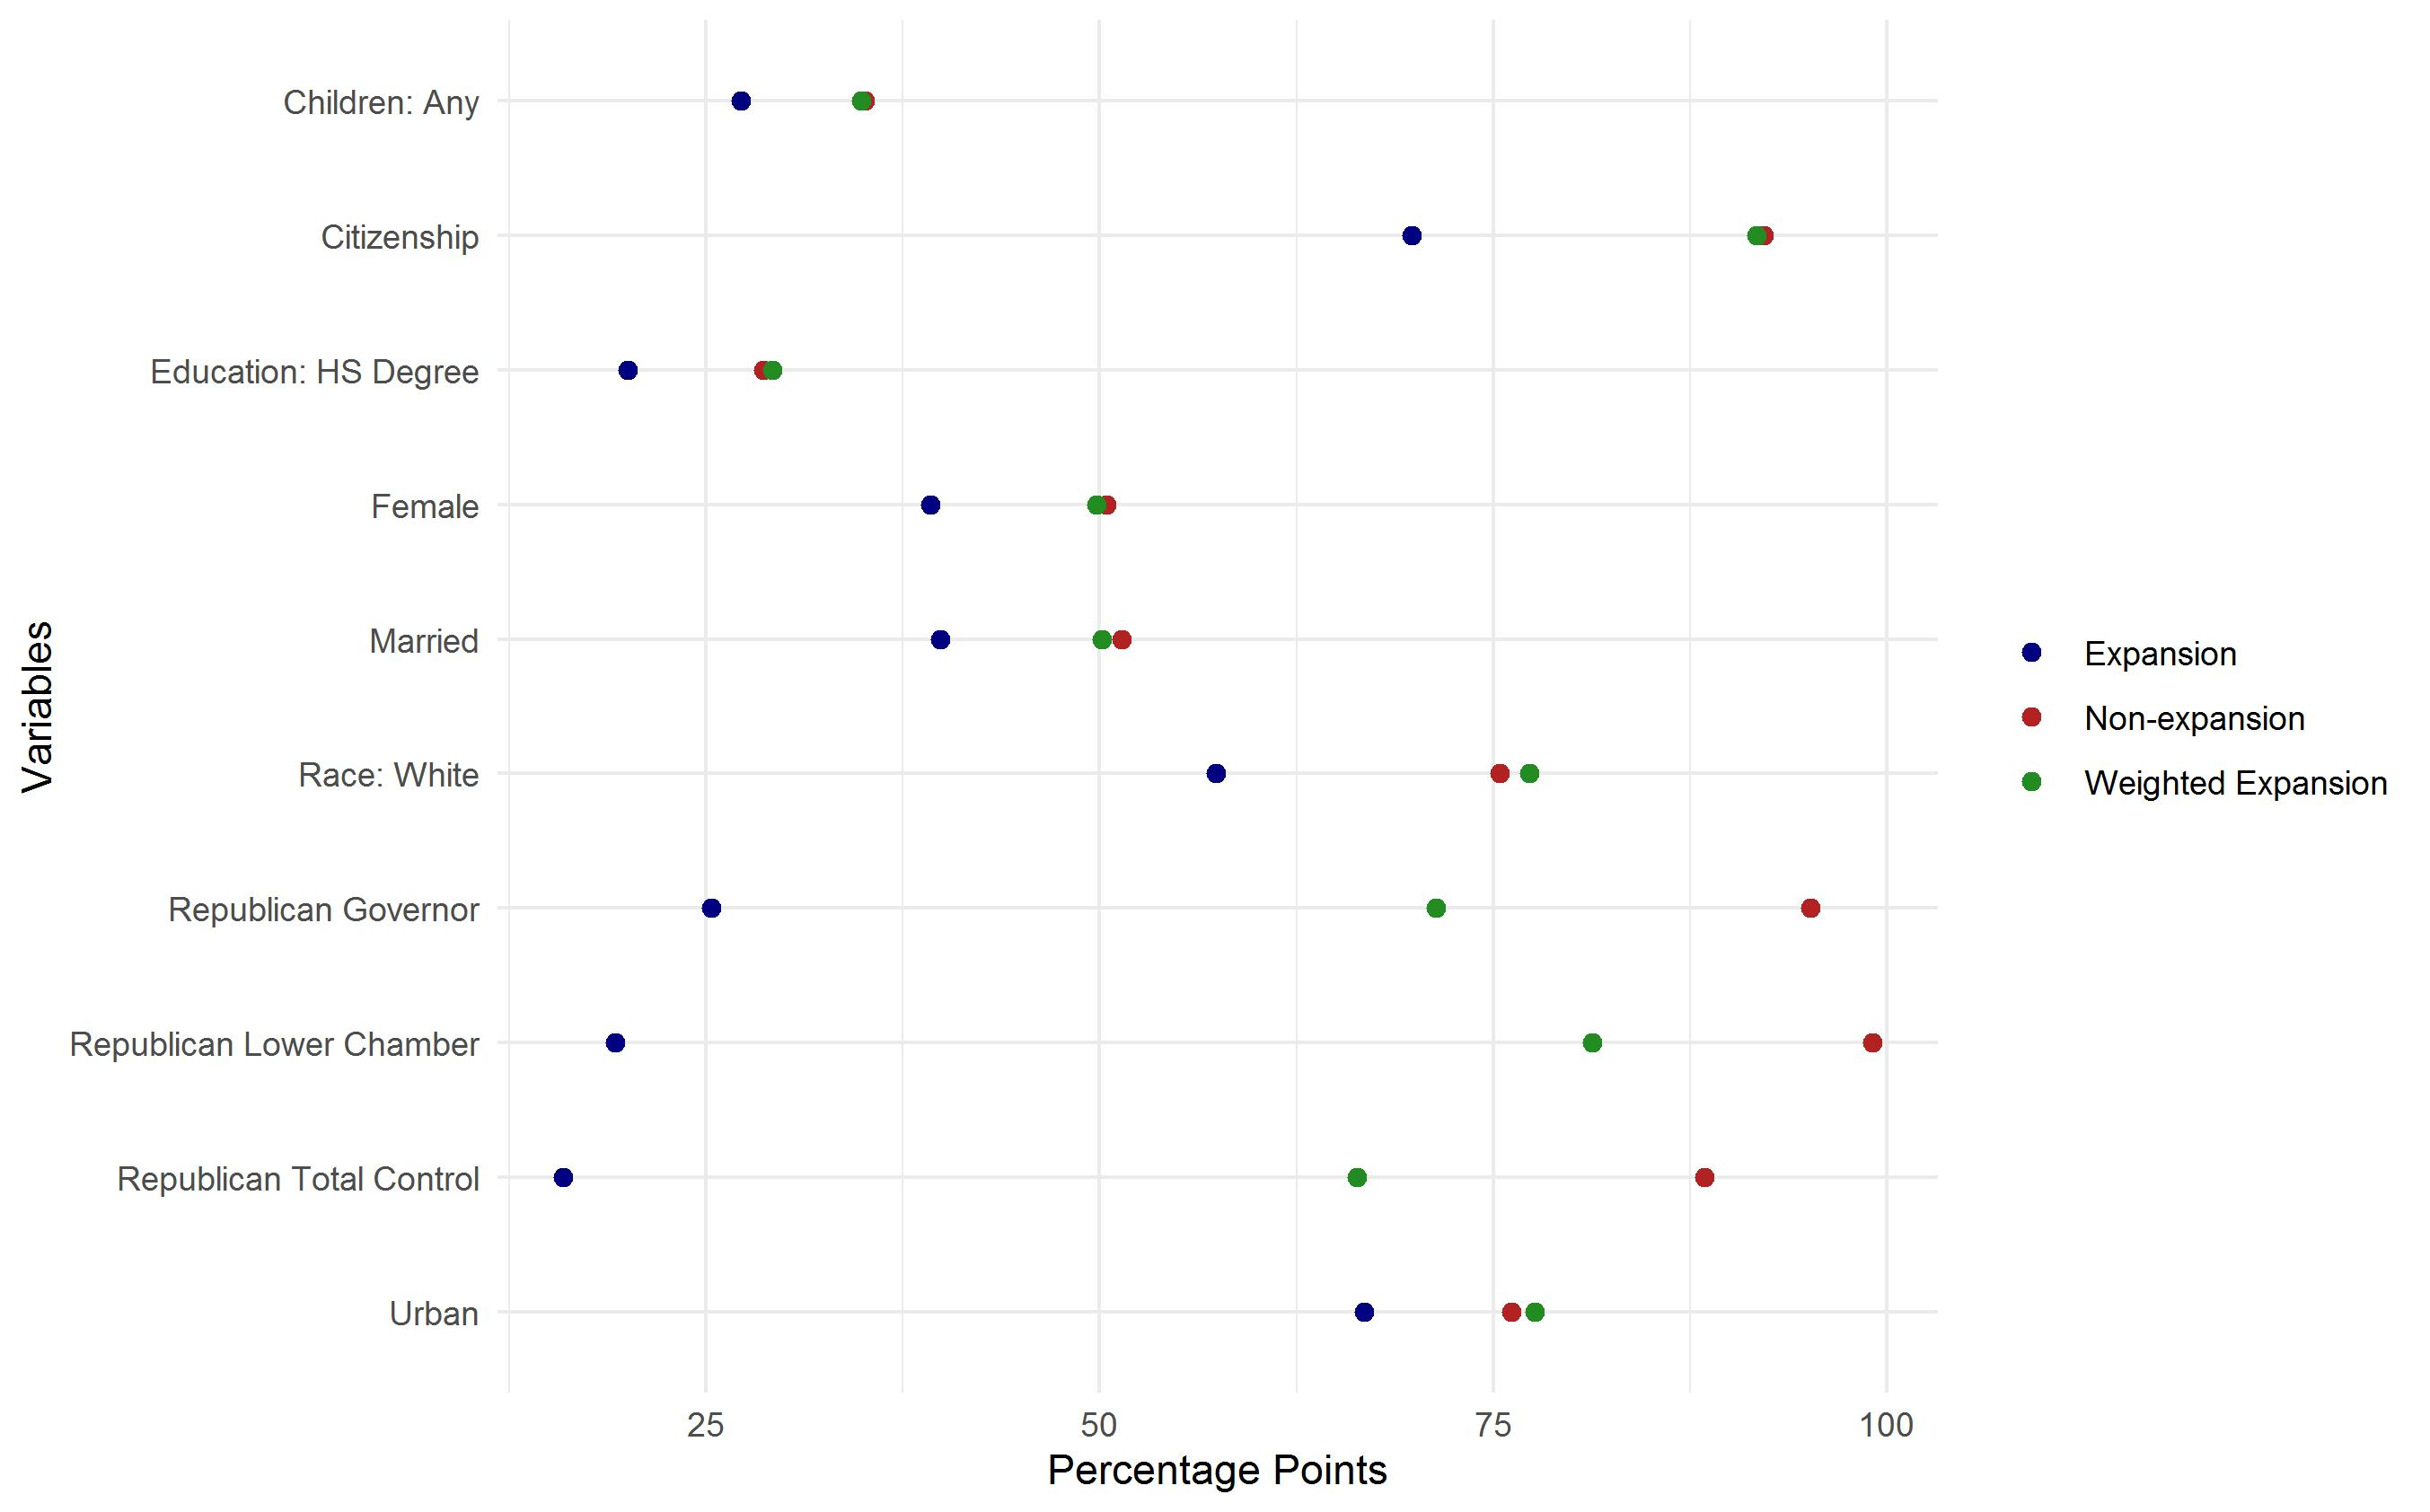
\includegraphics[scale=0.6]{images/balance-plot-largest10-unweighted.jpeg}
    \caption{Ten most imbalanced covariates: unweighted and weighted}
    \label{loveplot}
\end{center}
\end{figure}

Figure \ref{statewghts} shows the CPUMA-level weights by state; within each state the horizontal lines divide specific CPUMAs. Since we are balancing on Republican governance, we see that several Democratic-controlled states receive close to no weight, including Colorado, Connecticut, Hawaii, Iowa, Kentucky, Minnesota, Oregon, Rhode Island, and West Virginia. On the other hand, we see that over half of the weights are attributed to CPUMAs within Arkansas and Ohio.

\begin{figure}[B]
\begin{center}
    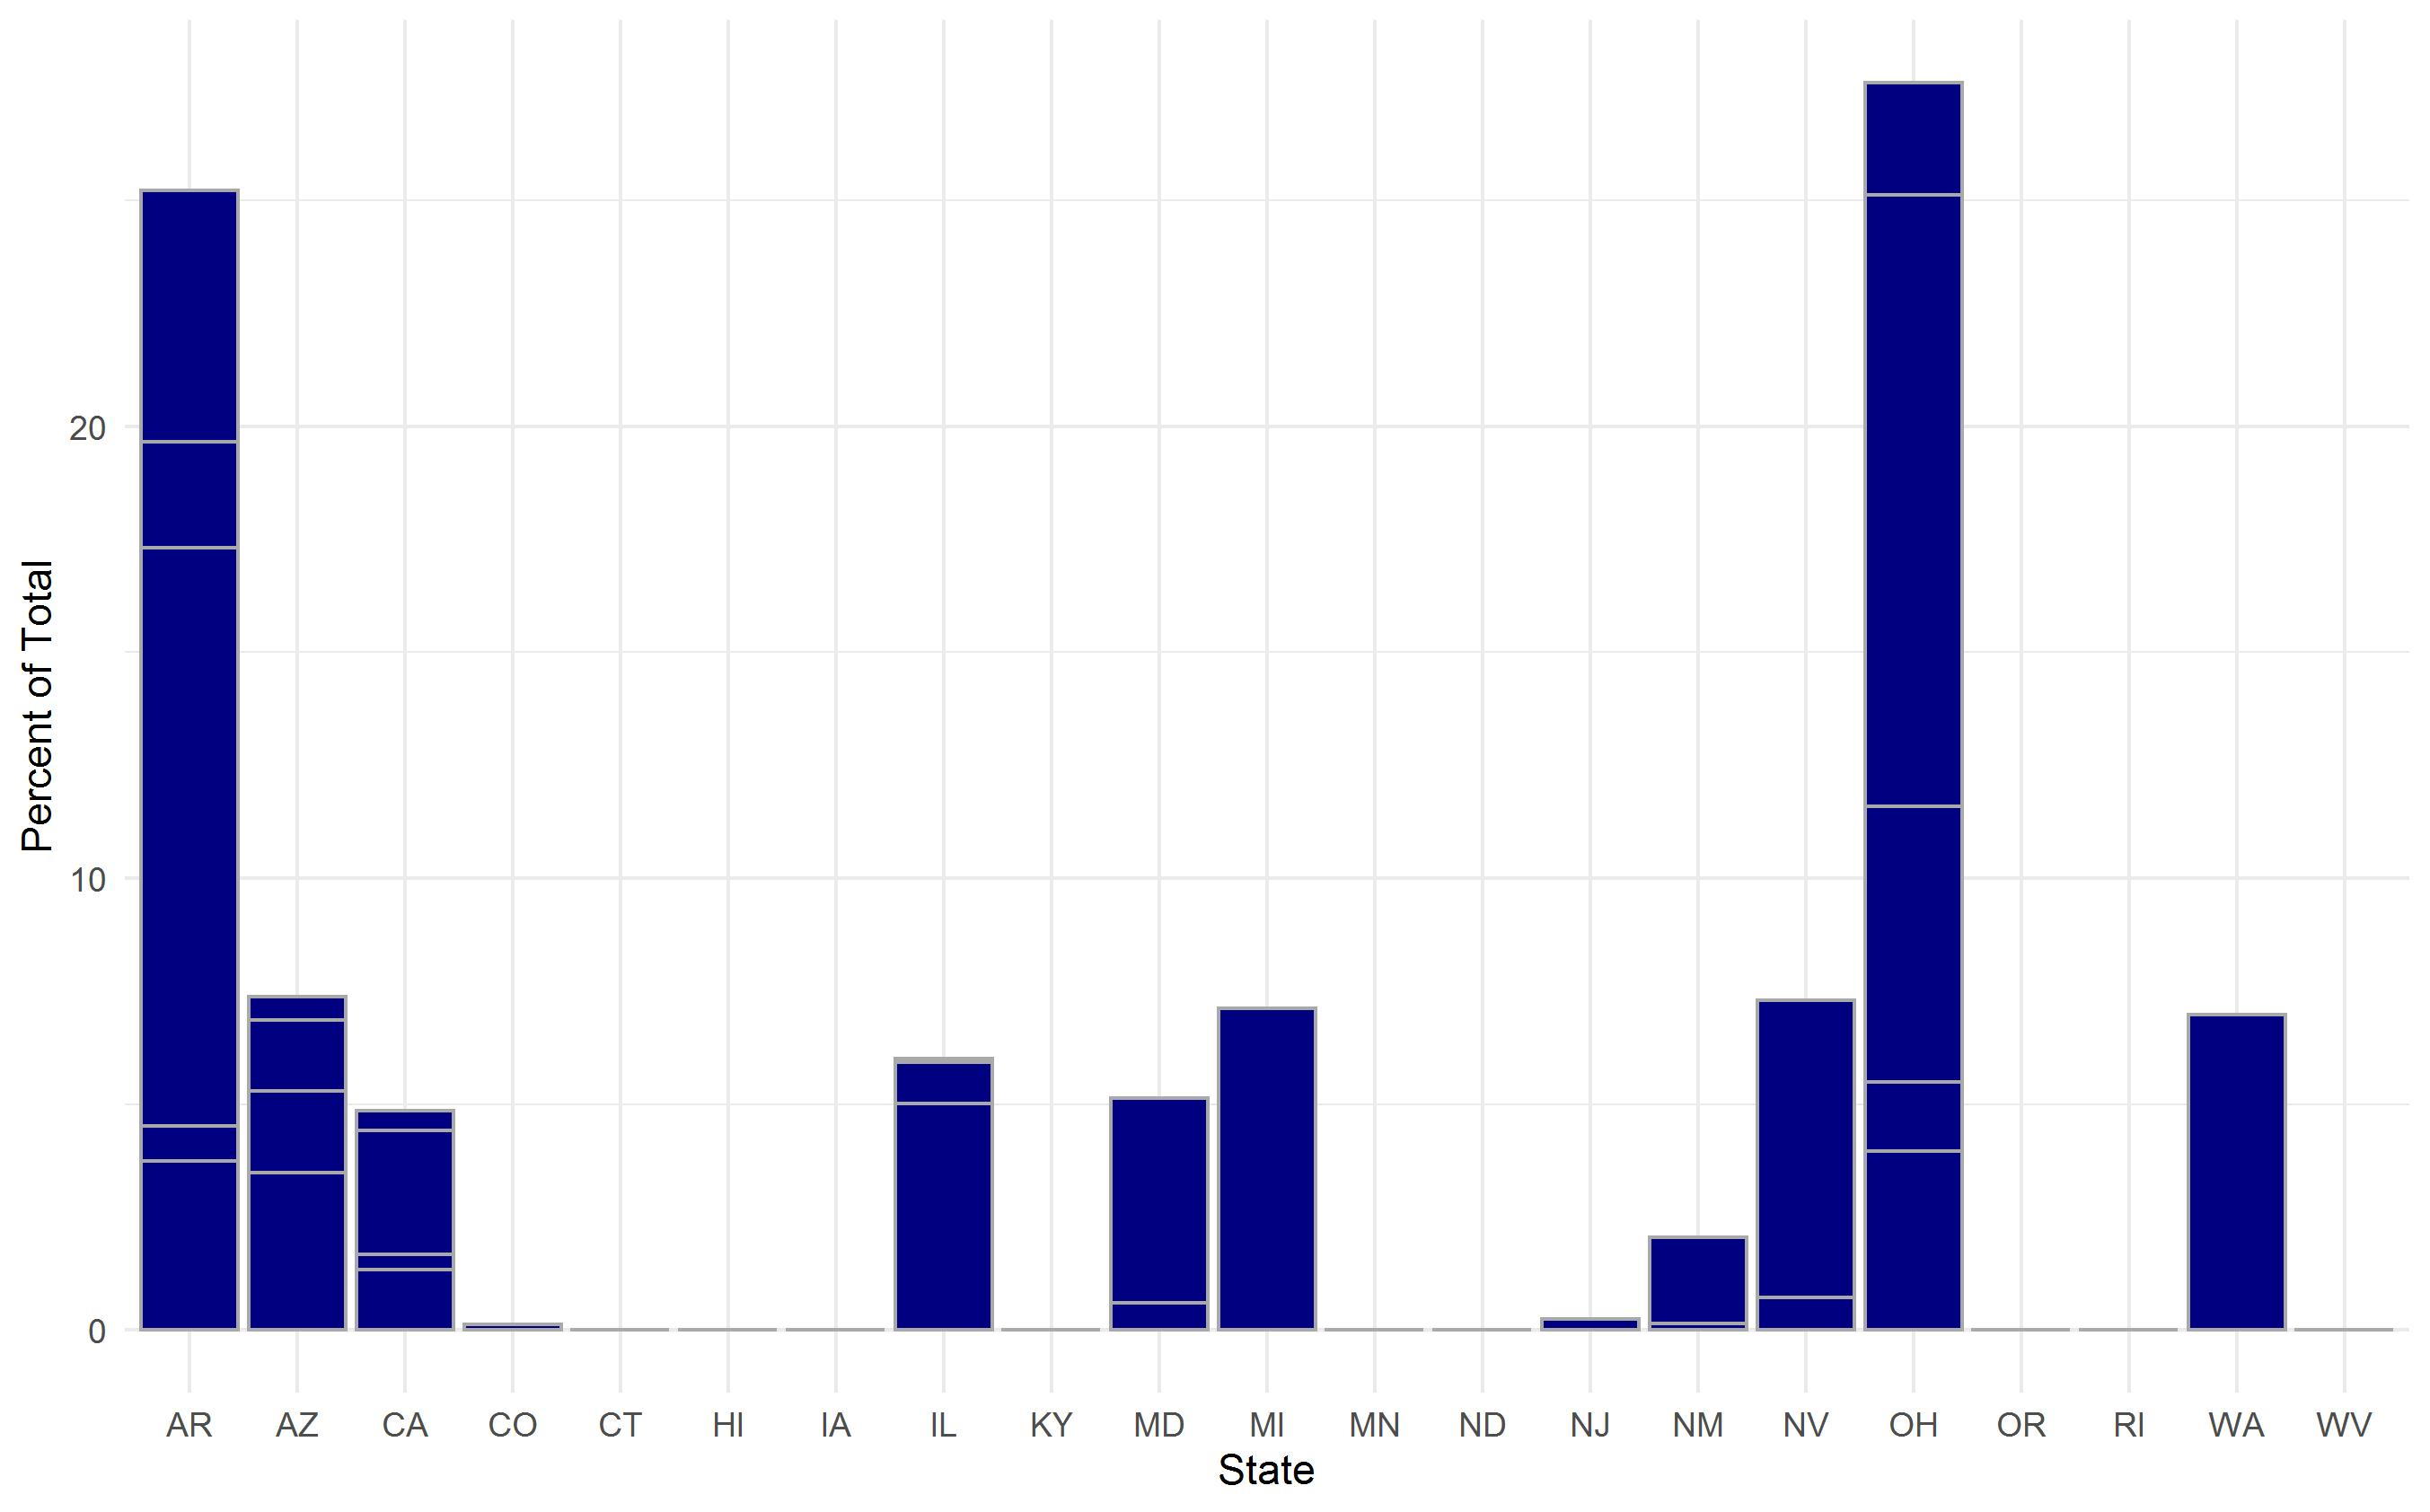
\includegraphics[scale=0.6]{images/cpuma-state-wgt-plot-new.jpeg}
    \caption{Total weights by CPUMA and State}
    \label{statewghts}
\end{center}
\end{figure}

Our bias-corrected estimator yields an estimated treatment effect of -2.18 percentage points (-1.31, -3.06). These estimates are virtually identical to the estimates using only the balancing weights (-2.21 (-1.32, -3.11)). Again these confidence intervals only account for the randomness in the survey we used to estimate the CPUMA-level covariates and outcomes, and the subsequent randomness in the weighting procedure. 

\begin{figure}[B]
\begin{center}
    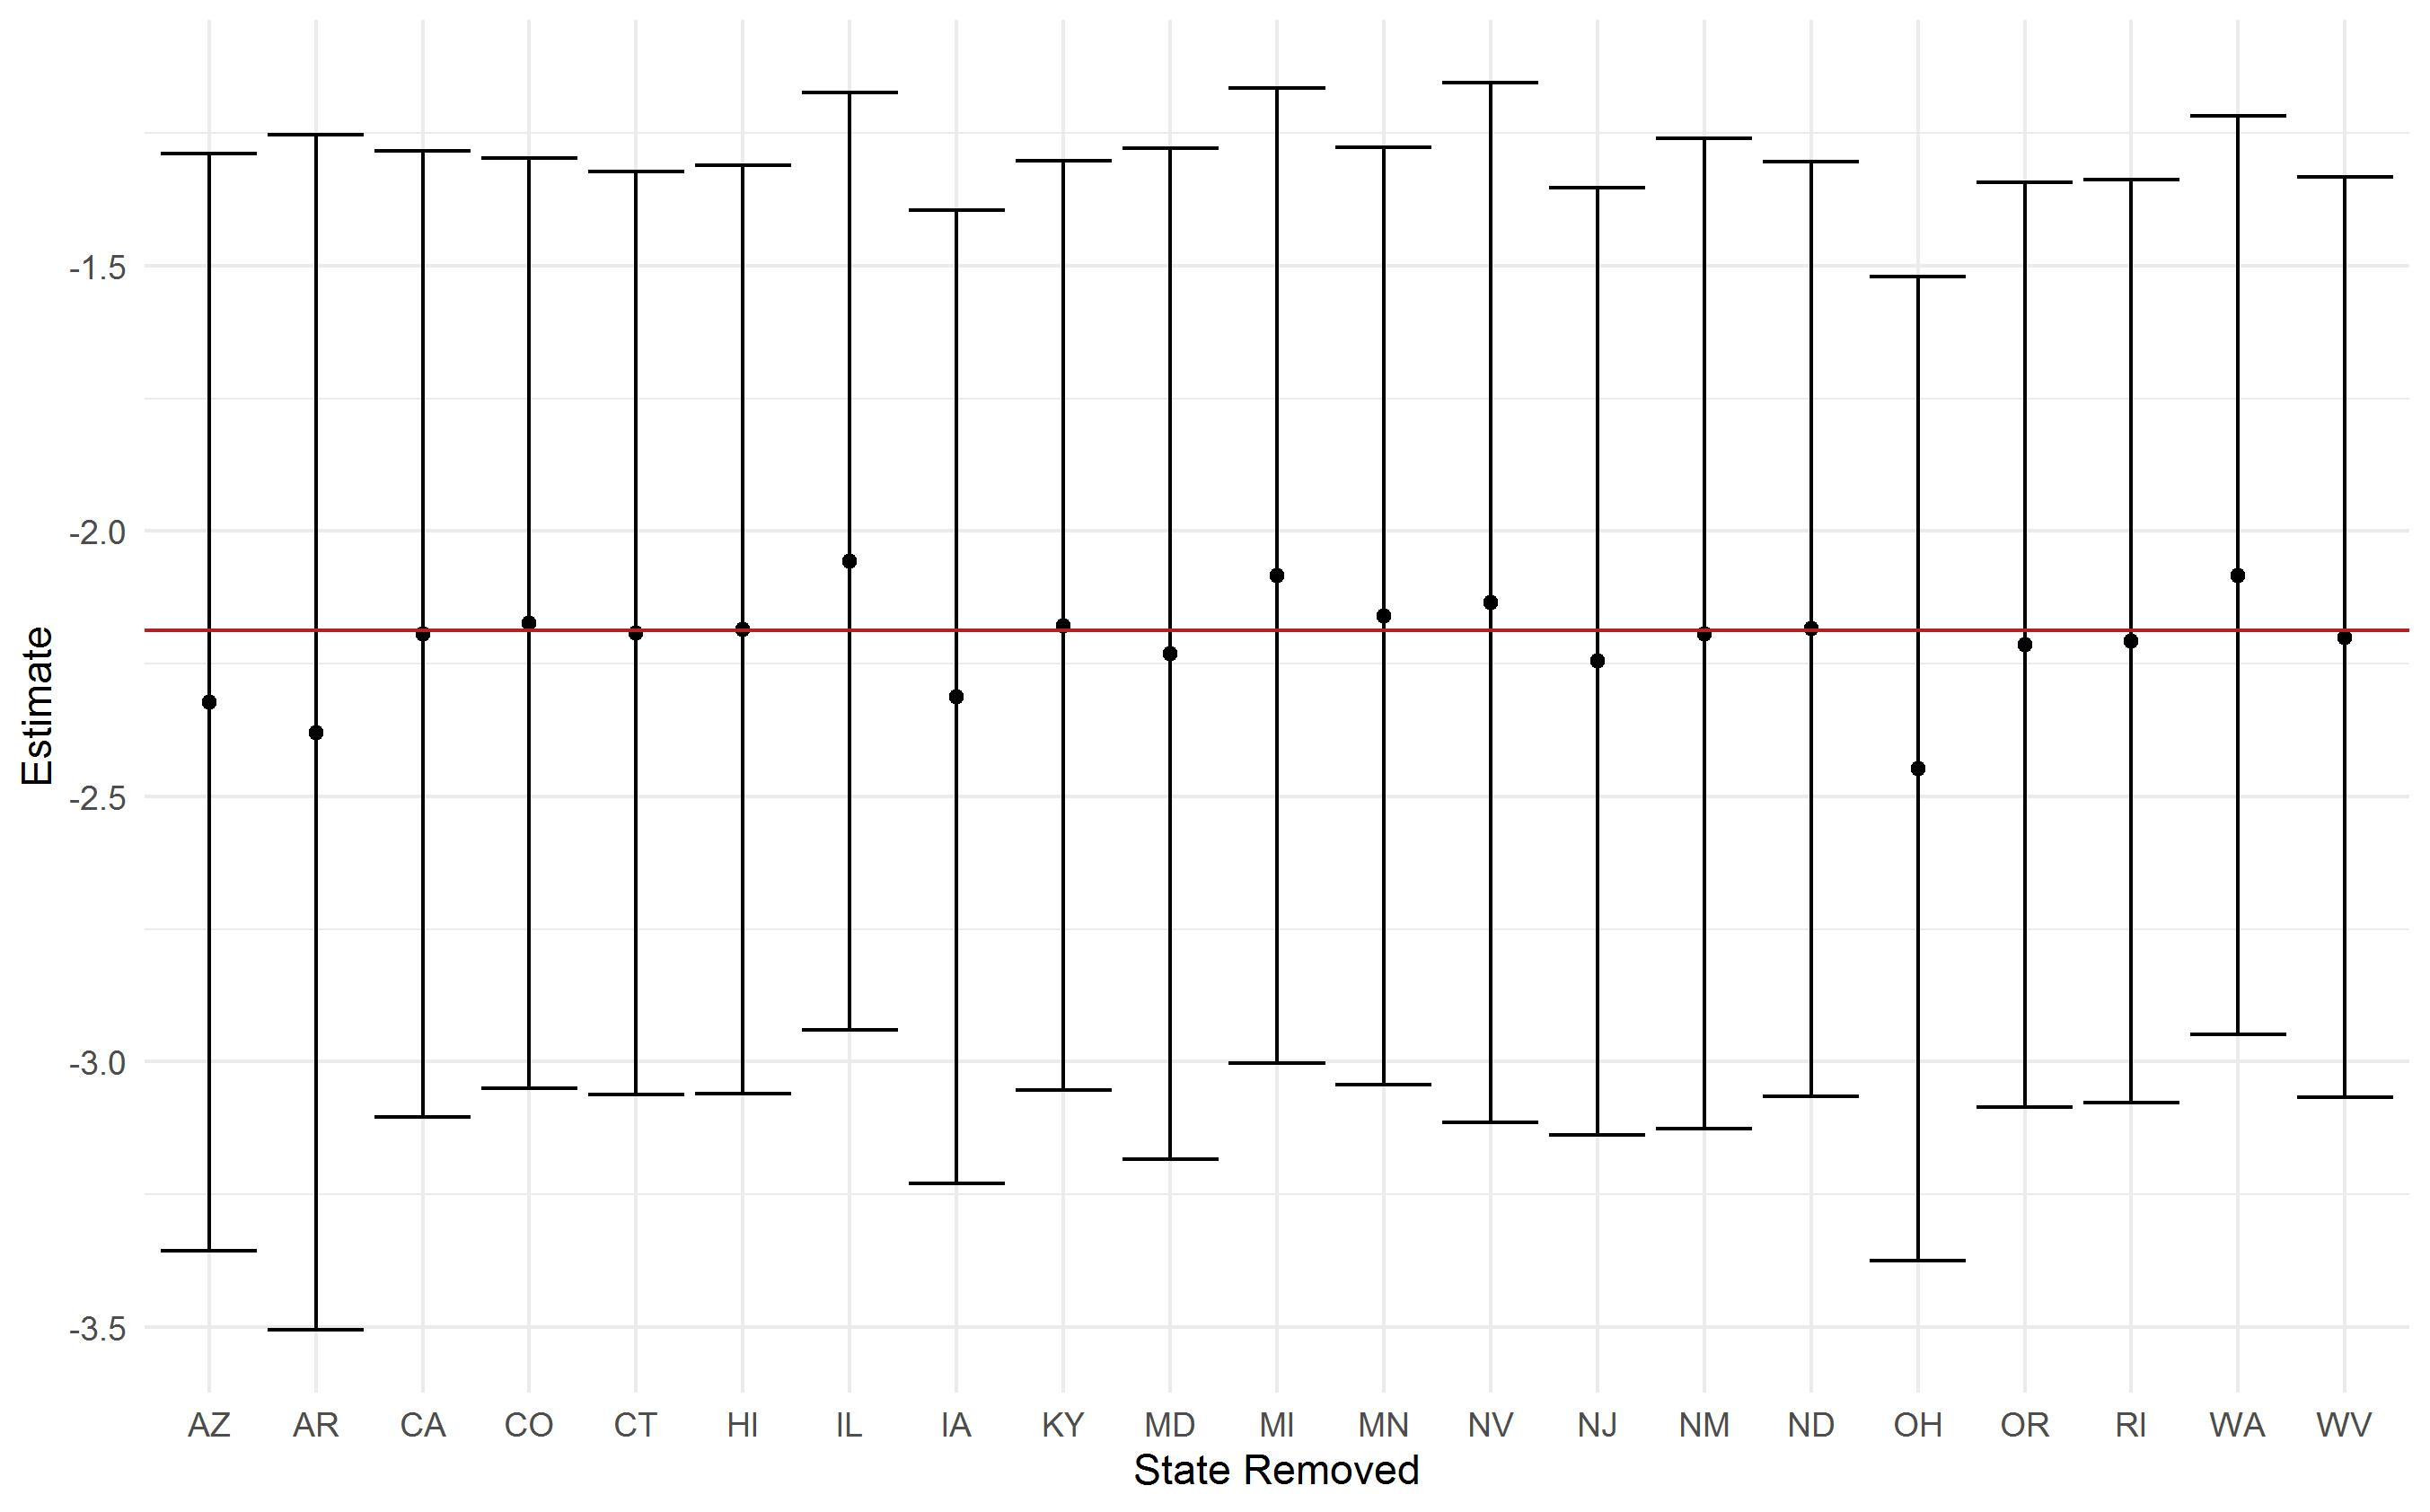
\includegraphics[scale=0.6]{images/loo-states-dr.jpeg}
    \caption{Leave-one-out state analysis: bias corrected estimator}
    \label{loostatesdr}
\end{center}
\end{figure}

We examine how sensitive our estimates are to particular states by removing one state at a time and rerunning the procedure. Figure \ref{loostatesdr} presents the results for the bias-corrected estimator (the weighting estimator results are very similar and are available in the Appendix). Unsurprisingly, removing the states that received zero weights made no impact on our estimates. The results were somewhat sensitive to the exclusion of Arizona, Arkansas, and Ohio; in particular, the treatment effect moves further away from zero when we remove these states. Overall, we see that the results appear to be slightly less sensitive to the removal of any particular state when using the bias correction.

Our last analysis examines how removing certain covariate groups in the weighting procedure changes the estimated contrast between the weighted treatment and control regions (ie the estimated treatment effect when all groups are included). We are especially interested how this contrast changes when we remove the Republican governance indicators: because we hypothesize that regions under Republican governed administrations should have lower Medicaid take-up rates, we expect that removing these covariates should move this estimate farther away from zero. We divide our covariates into six separate groups: pre-treatment uninsurance rates, pre-treatment unemployment rates, Republican governance indicators, racial demographics, education and poverty demographics, and other demographics (age, marital status, female, children, disability, urban). We then rerun the analyses excluding each group. Figure \ref{loocovsdr} displays the results. We see that removing the Republican governance indicators generates an estimate that is further away from zero than the estimated treatment effect, while removing other covariate groups results in estimated contrasts that are similar to the estimated treatment effect (results were similar when using the weighting-only estimator). 

\begin{figure}
\begin{center}
    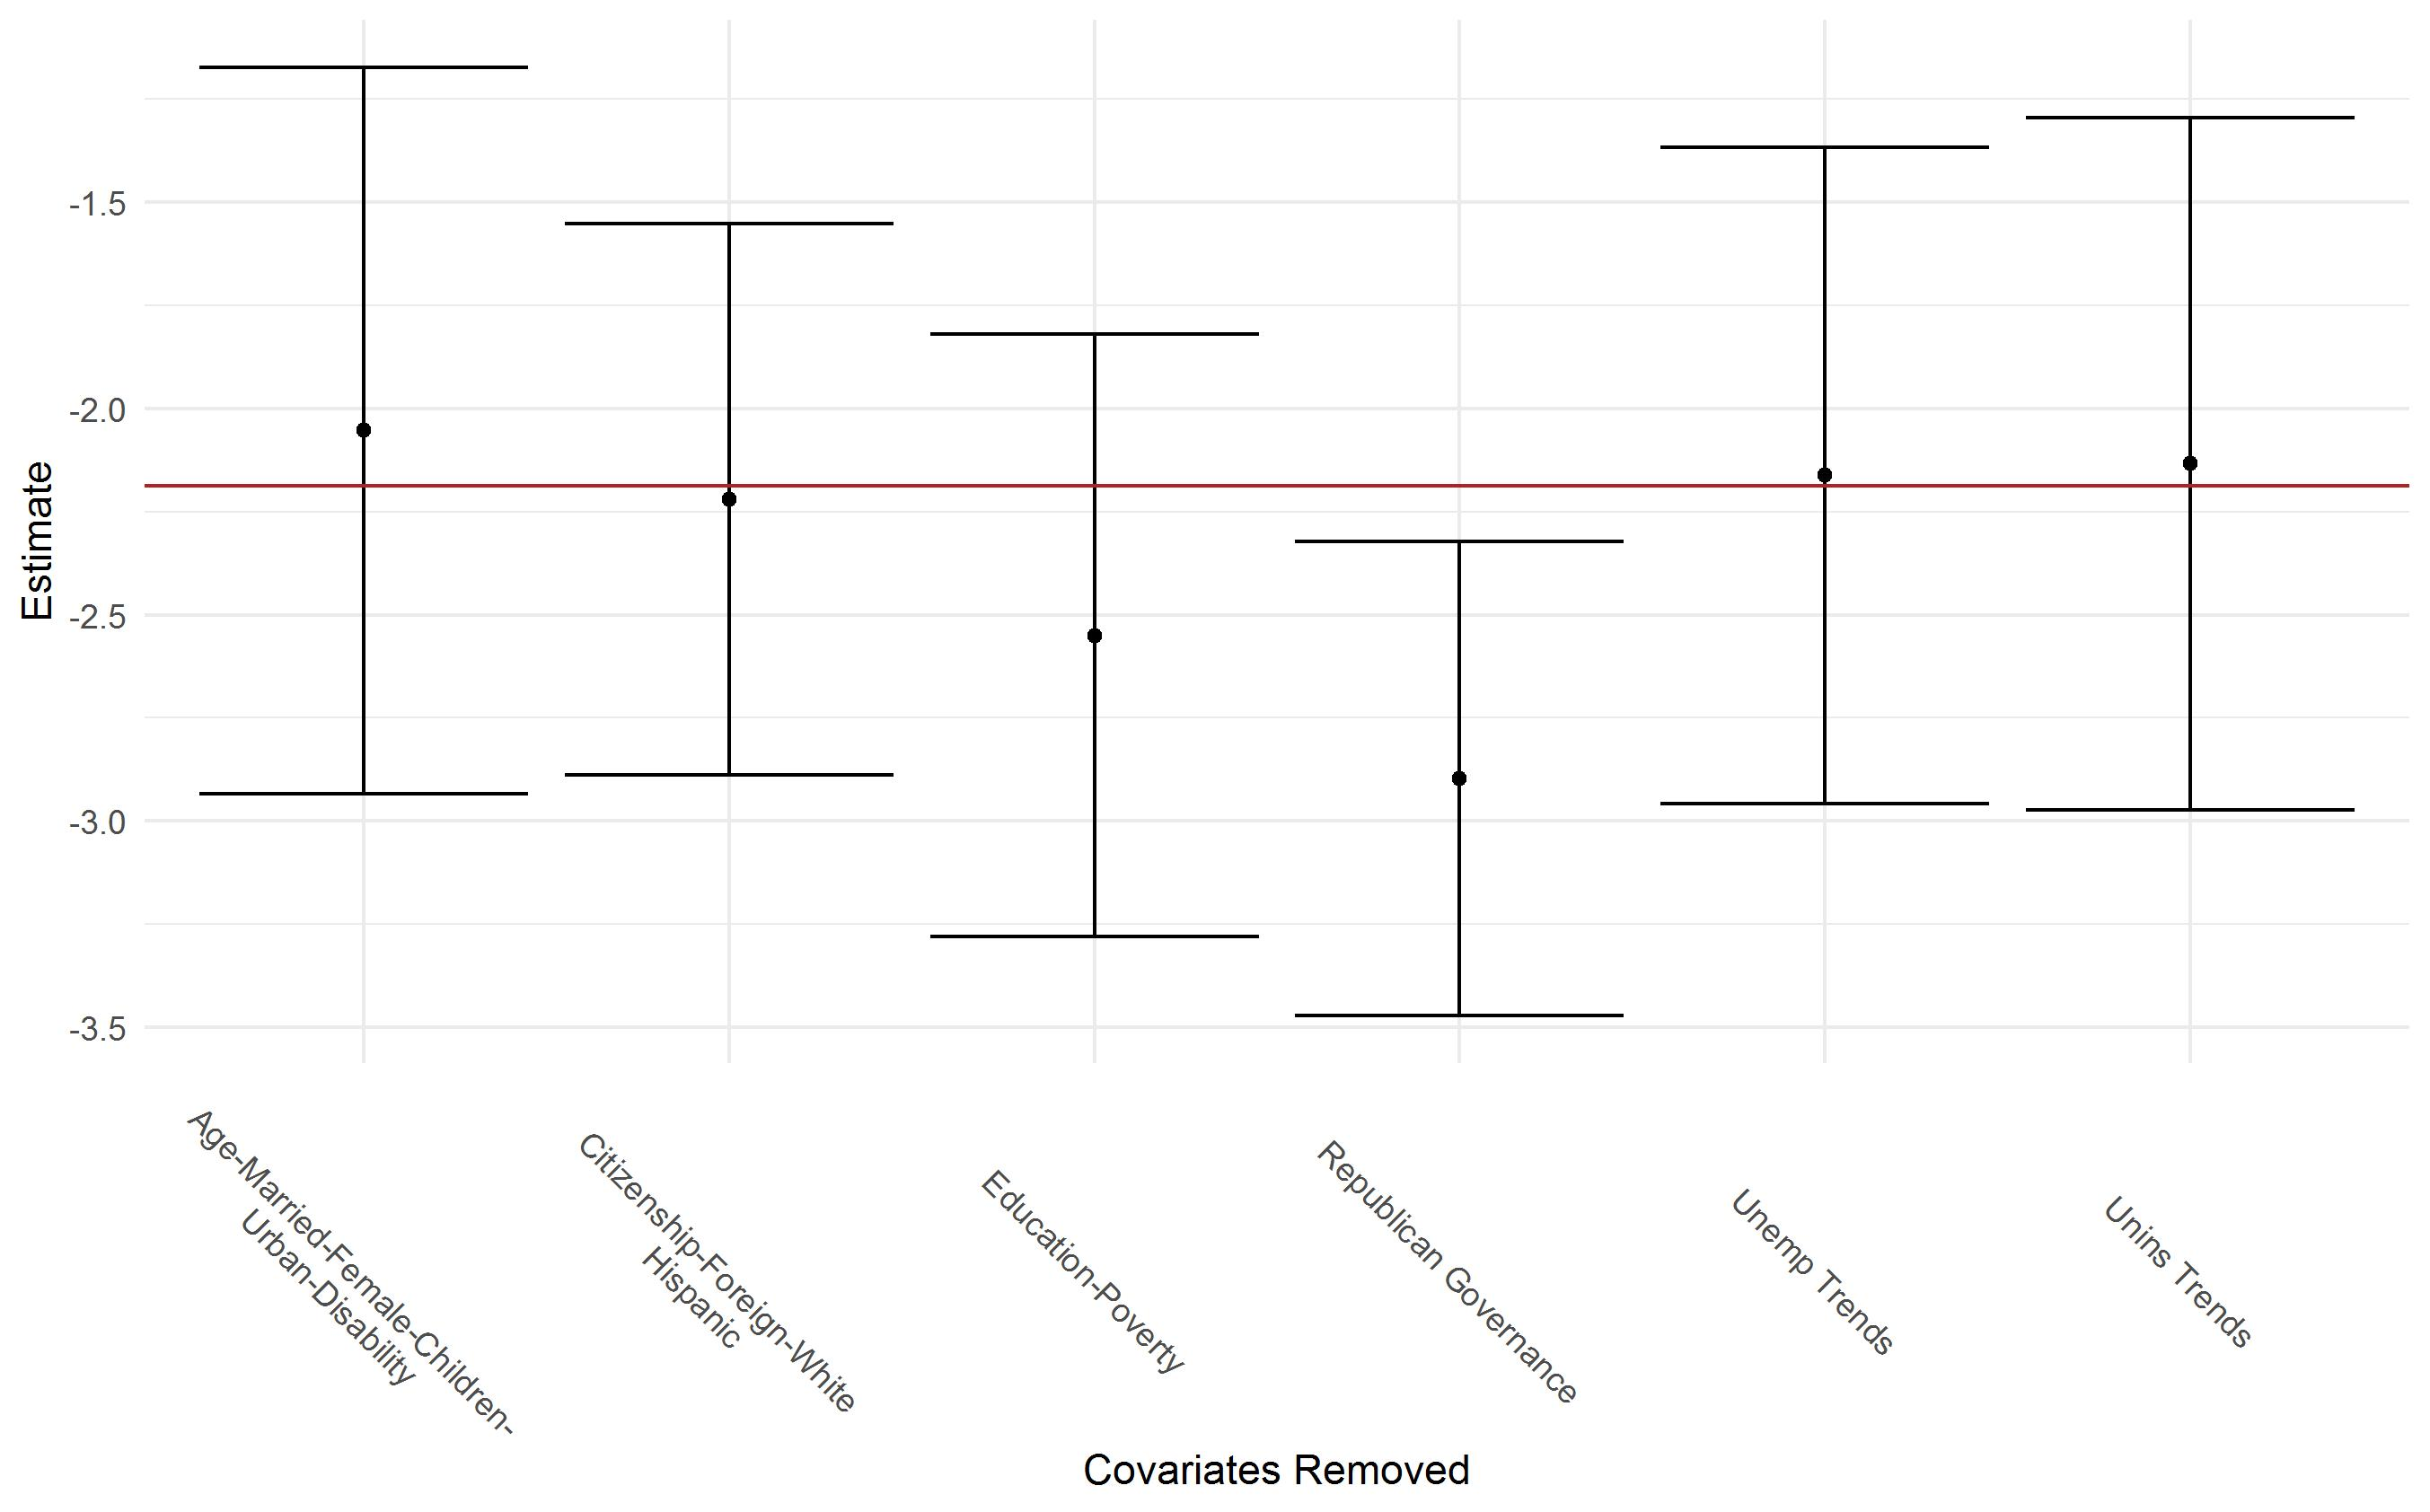
\includegraphics[scale=0.6]{images/loo-covariates-dr.jpeg}
    \caption{Leave-one-out covariate group analysis: bias corrected estimator}
    \label{loocovsdr}
\end{center}
\end{figure}

Overall these results suggest that Republican governance drives heterogeneity in the treatment effects. However, because regions from Ohio and Arkansas are largely drive our primary treatment effect estimates, it is possible that excluding these states may change this observed association. We therefore combine the leave-one-out covariate analysis with the leave-one-out state analysis to see how these estimated contrasts change. We see very similar results throughout, and that the covariate group with the strongest associated heterogeneity is the Republican governance indicators, which held regardless of the state excluded. Full results are available in the Appendix.

\subsection{Sensitivity Analyses}

We now examine the sensitivity of our results to violations of two key causal assumptions: (1) no anticipatory treatment effects, and (2) positivity.

Several states had partial limited expansions prior to 2014. Following \cite{frean2017premium}, we consider these states to be California, Connecticut, Minnesota, New Jersey, and Washington. We rerun our analyses excluding CPUMAs from all five of these states. We are unsure how we should expect this to affect our estimates: on the one hand, states that expanded early might have a smaller treatment effect after 2014 because they already enrolled newly eligible individuals. This would bias our previously estimated treatment effect upwards. On the other hand, if these states were also more motivated to enroll people in Medicaid, they might have larger post-exapnsion coverage gains, leading to a downwards bias. When removing these states, we estimate an effect of -1.97 (-0.96, -2.98). This is consistent with the latter story. However, when we run the bias-corrected version we estimate -2.27 (-1.48, -3.38), which is consistent with the former. Regardless, the confidence intervals largely overlap. Overall these results suggest that the bias from potential anticipatory treatment effects from these states was negligible. Our leave-one-out covariate analysis shows similar results to those in our primary analysis (results available in the appendix).

Our final analysis tests the sensitivity of our estimates to positivity violations. Because we were not able to get full overlap, our weighting estimators suffer some bias due to the imbalances, and our bias-corrected estimators rely on linearly extrapolating from our data. We therefore target a different treatment effect here -- the overlap treatment effect, using overlap weights proposed by \cite{li2018balancing}. Using logistic regression, we generate weights that exactly balance the means of the covariates between control and treatment group. The cost is that we now have a data-dependent treatment effect: the overlap average treatment effect, which represents the treatment effect within regions where there is covariate overlap. We are therefore changing the targeted causal parameter.

Figure 6 shows the expansion state, non-expansion state, and overlap weight covariate means, ordered by the largest difference between expansion and non-expansion states (limited to only the ten largest imbalances). We see that the overlap region is far more closely politically aligned with the non-expansion region. We also see that it is a less diverse and more rural area than either the expansion or non-expansion states, with fewer foreign born, urban residencies, and a much lower hispanic population. We also see that the pre-treatment uninsurance rates are also lower than either the overall expansion or non-expansion states (this is also true of the unemployment rates). In general we find that the average L2 distance between the expansion states and overlap region is 8.29 percentage points while it is only 2.91 between the non-expansion and overlap region. Since we found earlier that Republican governance seems to be the largest driver of effect heterogeneity, and the overlap region is more similar to the ETU than the ETT in this respect, we should expect that our estimate of the OATE is also more similar to the ETU than the ETT.

\begin{figure}
\begin{center}
    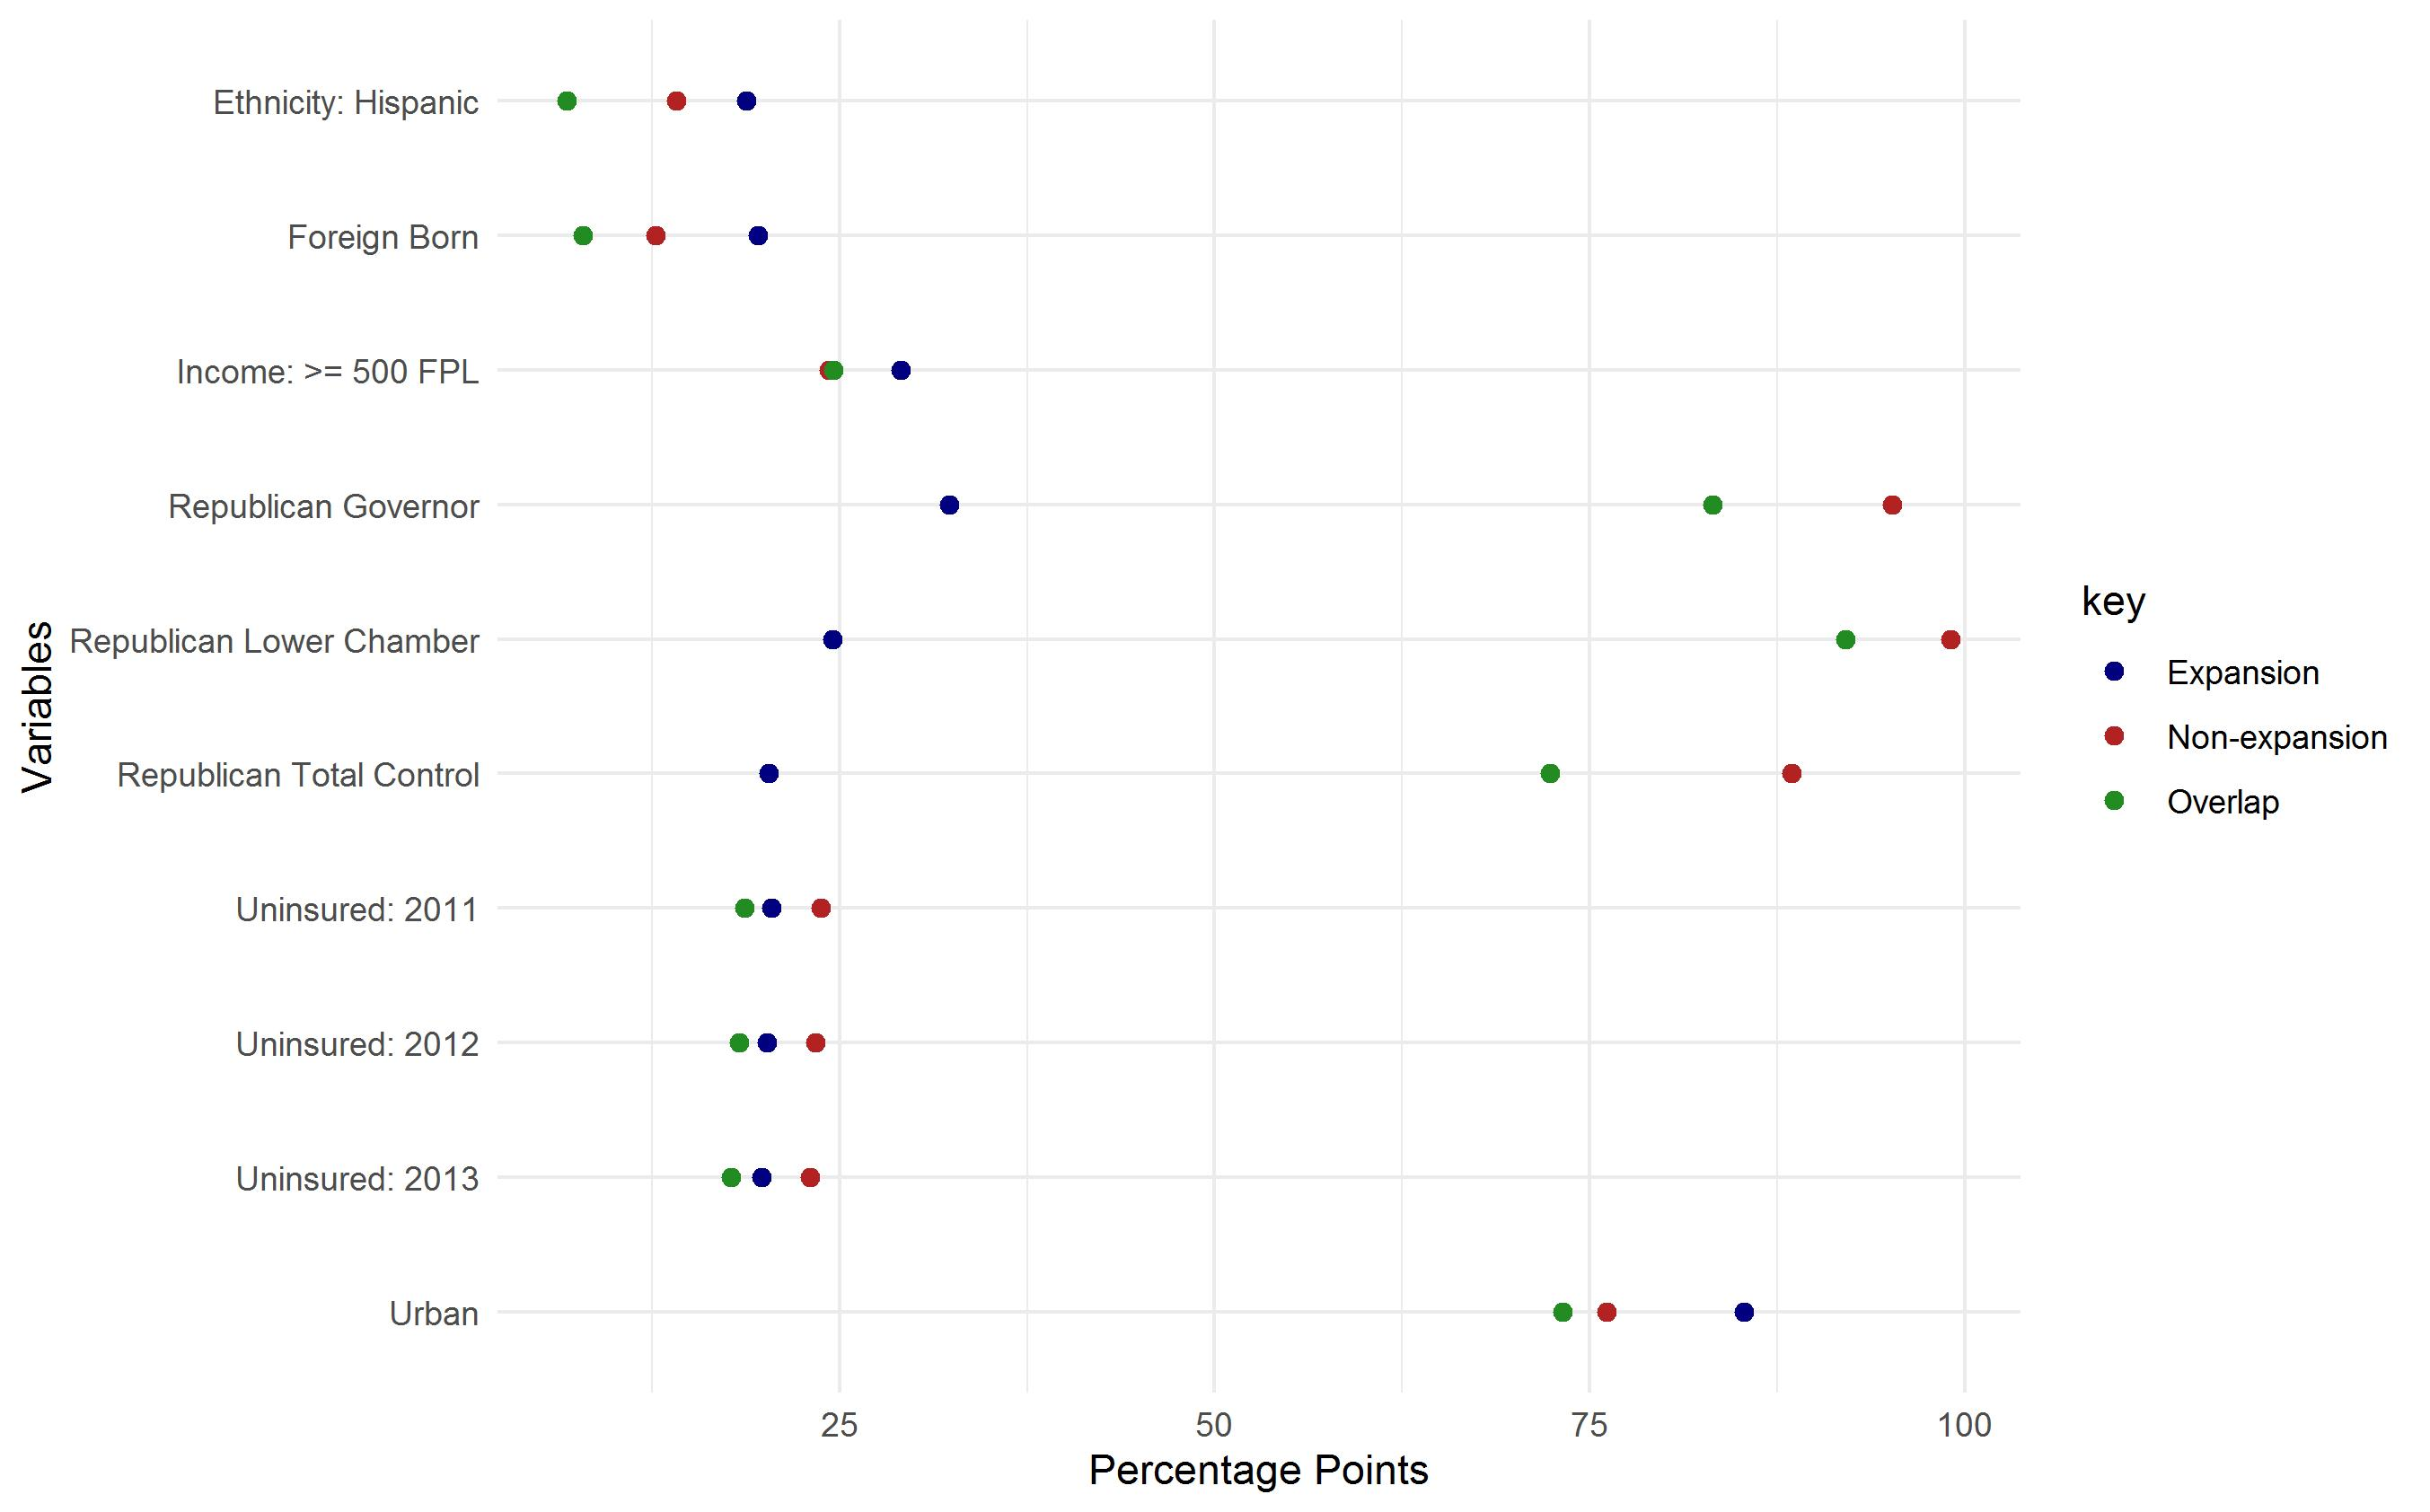
\includegraphics[scale=0.6]{images/oate-balance-plot-largest10-unweighted.jpeg}
    \caption{Ten most imbalanced covariates: unweighted and weighted}
\end{center}
\end{figure}

\ref{oatepref} shows the total percentage contribution of CPUMAs within each state to the overall OATE weights by treatment group. Notice that many of the expansion states are heavily downweighted, whereas the distribution across the non-expansion states is more uniform. In particular, we see that Ohio and Michigan constitute over 50 percent of this regions weights, while the Pennsylvania, Wisconsin, Missouri, and Florida represent over 50 percent of the non-expansion state weights.

\begin{figure}
\begin{center}
    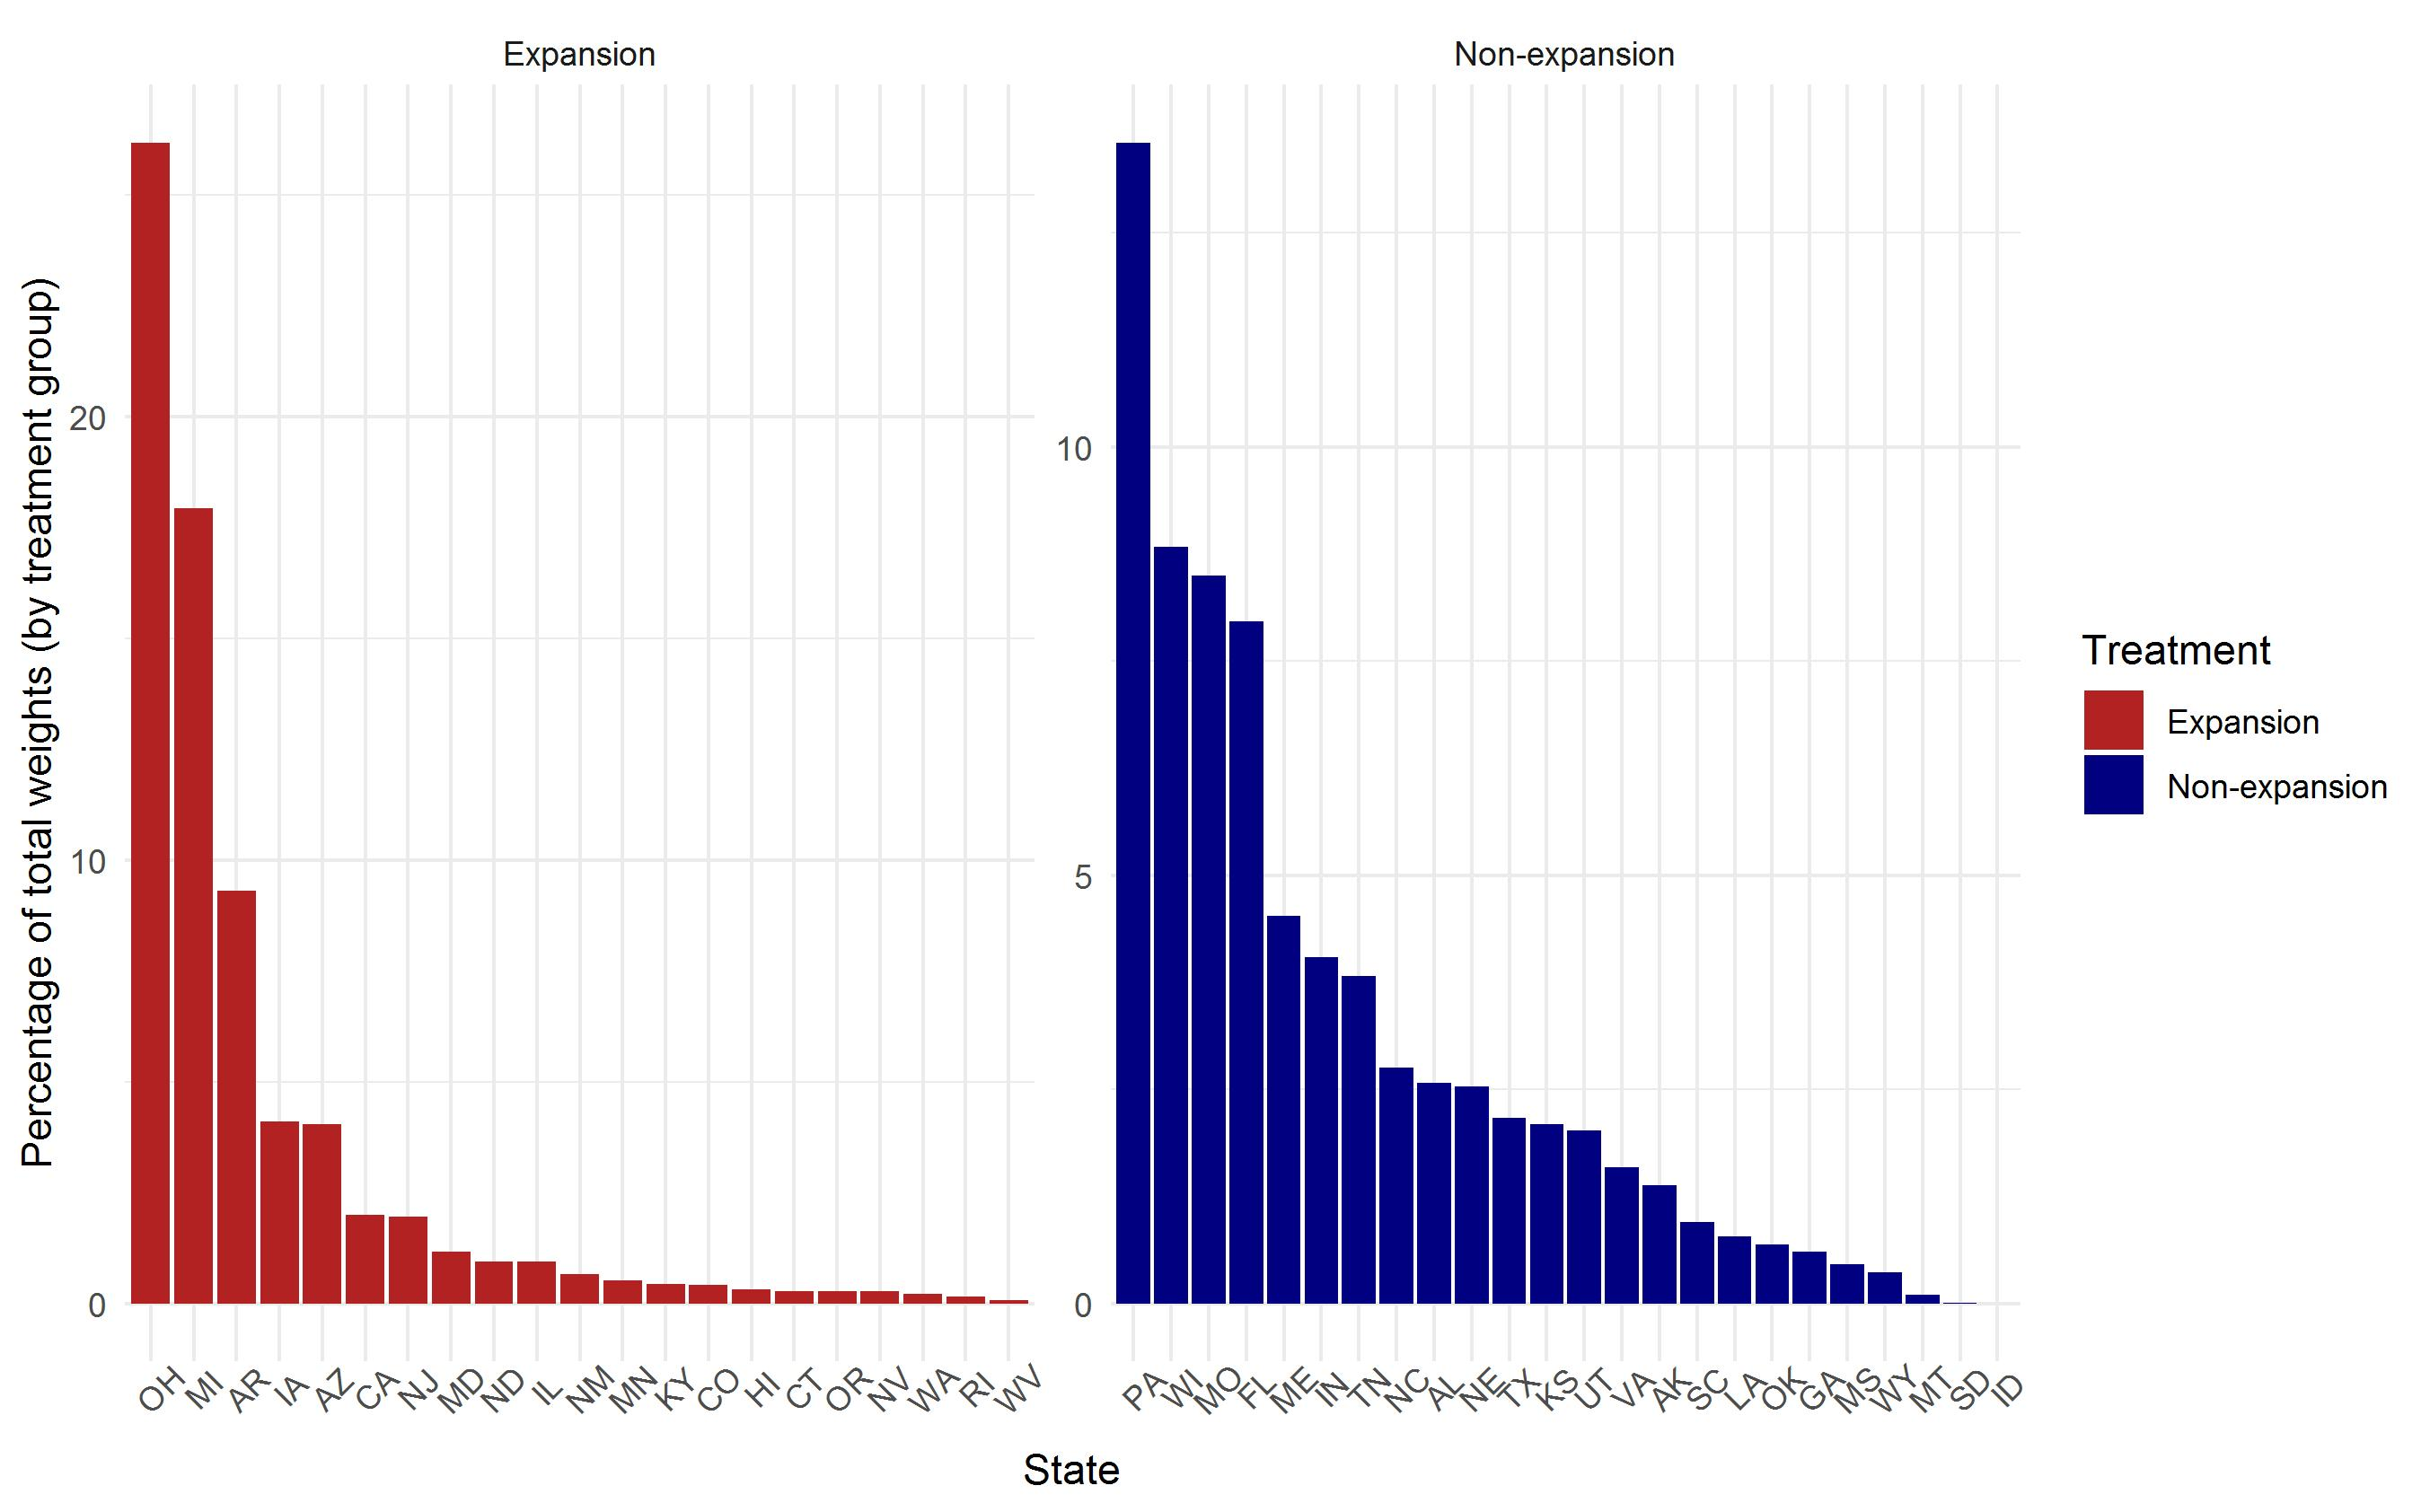
\includegraphics[scale=0.6]{images/overlap-weights-state-weights.jpeg}
    \caption{Overlap weights: state total contribution to estimator}
    \label{oatepref}
\end{center}
\end{figure}

We estimate that the OATE is -2.02 (-1.63, -2.41), which is closer to zero than our preferred bias-corrected estimator of the ETU (-2.19). Why might this estimate be closer to zero than the ETU? One possible reason is because the pre-treatment uninsurance rates are already relatively low: perhaps this reflects a floor effect. That is, because the uninsurance rates are already relatively low relative to either the expansion or non-expansion regions, it is harder to reduce them. In general though the confidence intervals of the OATE and ETU overlap somewhat, suggesting that this difference may also simply be due to sampling variability in the ACS.

We next conduct the same set of sensitivity analyses as before. We find that our estimated treatment effect is virtually unchanged when we remove the potential early expansion states(-2.01 (-1.61, -2.40)). \ref{loostate} shows that results are quite insensitive to removing any particular non-expansion state, though they appear most sensitive to Ohio, Iowa, and Arkansas. Our leave-one-out covariate group again shows the negative association between Republican governance and the magnitude of the treatment effect. The leave-one-out covariate group by state analysis is available in the Appendix and is consistent with these results, again showing that Republican governance is negatively associated with the estimated treatment effect.

\begin{figure}
\begin{center}
    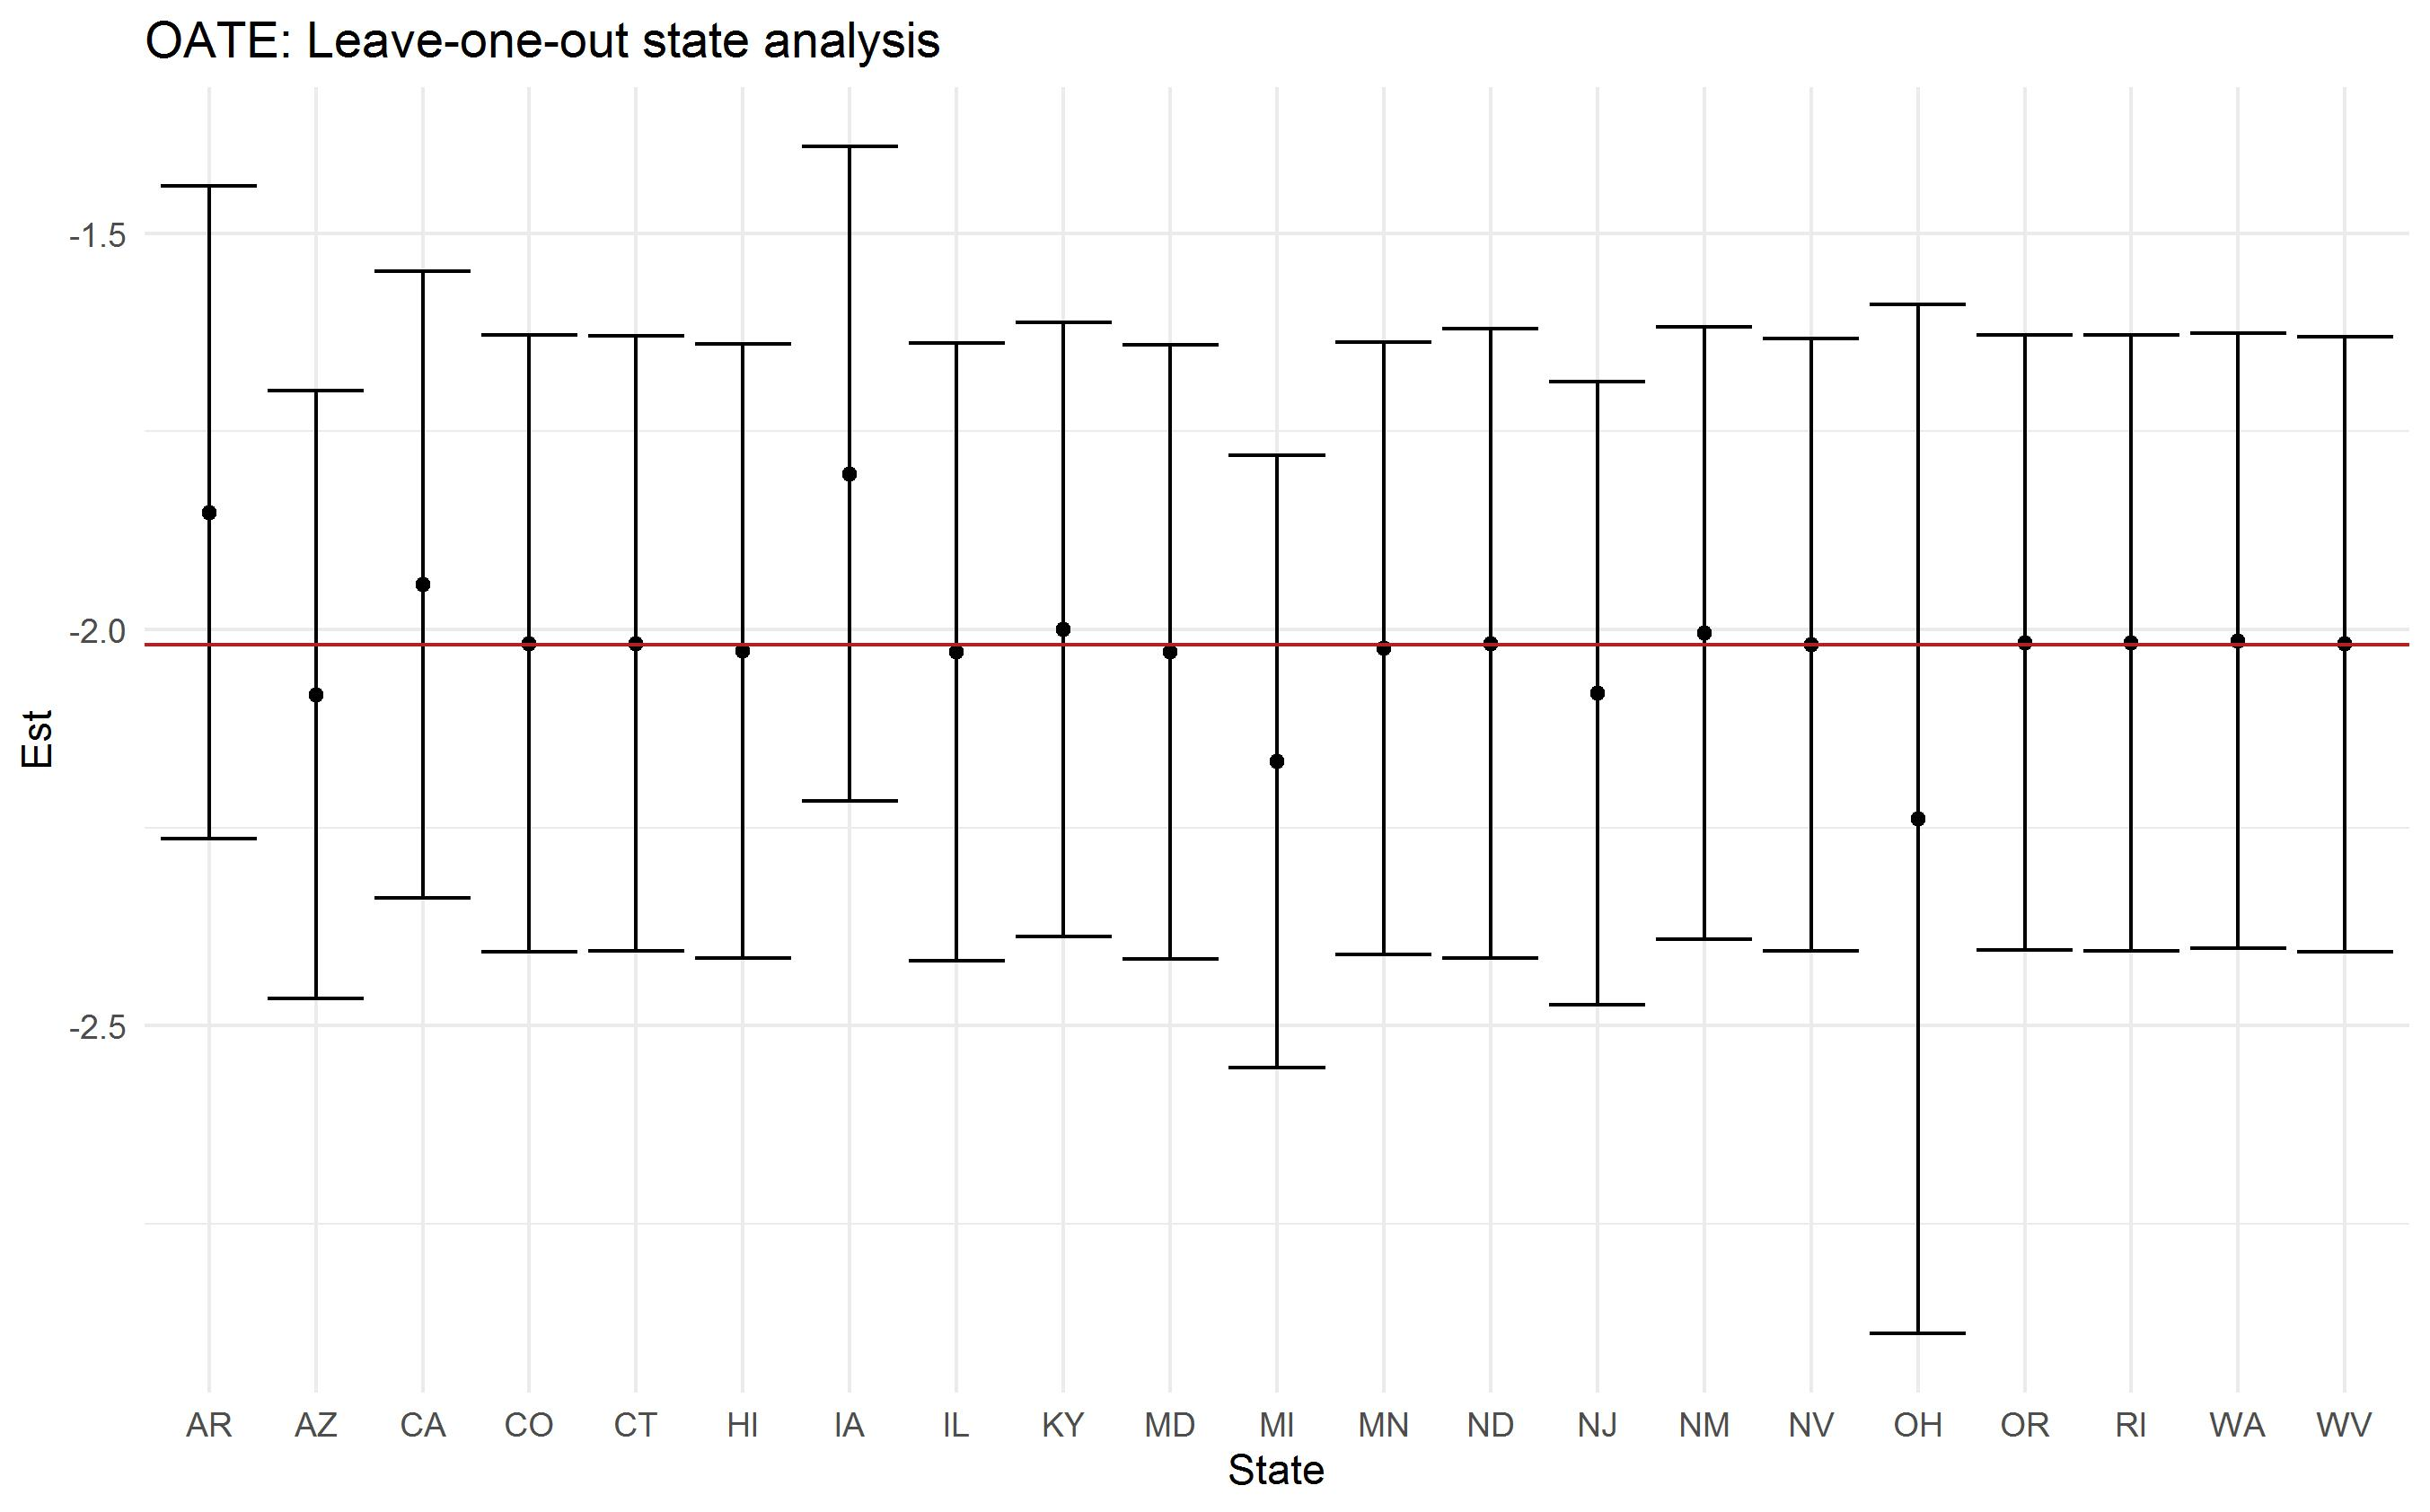
\includegraphics[scale=0.6]{images/oate-loo-state.jpeg}
    \caption{OATE leave-one-out state analysis}
    \label{loostate}
\end{center}
\end{figure}

\section{Discussion}

We estimate that had states that did not expand Medicaid in 2014 expanded their programs, they would have seen a 2.18 (1.31, 3.06) percentage point decrease in the adult uninsurance rate. Existing estimates place the ETT between -3 and -6 percentage points; these estimates vary depending on the targeted sub-population of interest, the data used, and the modeling approach (see, eg, \cite{courtemanche2017early}, \cite{kaestner2017effects}, \cite{frean2017premium}). This estimate is therefore closer to zero than these  papers, supporting our original hypothesis that the treatment effect on non-expansion states would be smaller in absolute magnitude. Moreover, we also find that we are likely to estimate treatment effects that are larger in absolute magnitude when allowing our comparison states to include states with more Democratic governance. This suggests that the differing political composition of the expansion versus the non-expansion states may explain these differences.

We also contribute to the methodological literature by extending the synthetic controls literature to estimate the treatment effect on the untreated. The key challenge is that we are trying to predict treatment response rather than the outcome absent treatment. We assume no unmeasured confounding and a linear and additive outcome model and generate weights that approximately balance the mean covariates of the expansion states to match the mean covariates of the non-expansion states. Unlike when estimating the treatment effect on the treated, we cannot use pre-treatment outcomes to conduct variable selection, run placebo tests, or train our model in some other way. This is a fundamentally more difficult problem that requires greater modeling assumptions.

Our study's approach also has bearing on estimating the ETT using a differences-in-differences to study the 2014 effects of Medicaid expansion. In particular, the consistent positive association between Republican governance and the estimated contrast between treatment and control states suggests that existing studies that fail to account for the interaction of treatment with measures of governance may incorrectly estimate the targeted treatment effects. We also find that there is likely insufficient overlap to account for these interactions without extrapolating from the data, and we show the ETU requires less extrapolation than the ETT with respect to these covariates. The primary estimand in the existing literature is instead the effect of treatment on the treated (ETT). While it may be tempting to extrapolate these findings to estimate the ETU (see, eg, \cite{miller2019medicaid}), this may lead to inaccurate inferences due to the heterogenous economic, demographic, and political characteristics between these groups of states.

Given that the effects of Medicaid expansion are primarily mediated through insuring the previously uninsured, we can assume that if the ETU were closer to zero than the ETT, then further downstream effects that grow monotonically with the number of insured would attenuate. For example, \cite{miller2019medicaid} use their estimate of the ETT to project that had all states expanded Medicaid in 2014, 15,600 deaths would have been avoided during their study's time-period. If we believe that the ETT were further away from zero than the ETU, we should expect that this number is an overestimate. Directly estimating the ETU in this context can therefore also help us better model interesting downstream effects mediated through increasing the number of insured individuals.

Our results come with the following caveats: (1) we rely on parametric assumptions about the outcome model to estimate our causal effect; (2) our identification assumes no unmeasured confounding, which is a relatively strong assumption; (3) spillovers across states might bias our estimates (and in general without redefining the causal estimand we cannot sign this bias); and (4) our variance estimation only accounts for the uncertainty in the ACS survey sampling. 

We conclude by discussing the policy implications of these findings. First, we note that a reduction of adult uninsurance rates by -2.18 percentage points in represents approximately an eleven percent reduction in the pre-existing uninsurance rate for non-expansion states. This estimated treatment effect is closer to zero than corresponding estimates of the ETT (see, eg, \cite{courtemanche2017early}). We may therefore expect that downstream effects that move away from zero monotonically with the number of uninsured are also closer to zero than estimates of the ETT. For example, \cite{miller2019medicaid} estimate that if their set of non-expansion states had expanded Medicaid during their study period, they would have avoided 15,600 deaths. Because these estimates were based on projecting the ETT onto non-expansion states, assuming that avoided deaths increase monotonically with the number of uninsured, our results suggest that this figure may be an overestimate.

Second, we emphasize that the positive association we find between governance and the estimated treatment effect is only an association: this finding does not imply, for example, that states with Republican governments in general make Medicaid enrollment more difficult relative to Democratic states. However, this finding does not rule out this possibility either. Even if this causal story were true, then it is also a normative judgment whether this finding is a ``good'' or a ``bad'' result. To evaluate the policy implications, we compare this result against Congress's goal in implementing Medicaid expansion in the 2010 ACA, which was to increase health insurance coverage. Measured against this goal, this finding suggests that leaving states to implement individual enrollment schemes likely achieves sub-optimal results. By this metric, ``better'' federal policies might encourage states to adopt some form of automatic Medicaid enrollment, or to make Medicaid enrollment easier in some other way.

On the other hand, it may also be the case that Republican governed states in 2014 were also more culturally conservative, and people may have been less likely to enroll in Medicaid due to social stigma and/or personal beliefs about the welfare state (\cite{sommers2012understanding}). If this remains true today, then Republican governments that are committed to expanding access to health care to low-income individuals may again wish to consider policies such as automatic enrollment to help mitigate these effects. Lastly, for Republican administrations who do not see coverage expansion as an important goal of Medicaid expansion, this finding may represent no policy problem at all.

\section{Conclusion}

This is the first study to directly estimate the foregone coverage expansions of Medicaid Expansion on states that did not expand Medicaid in 2014. We also contribute to the methodological literature on synthetic controls by clarifying the assumptions required to use longitudinal data to estimate the ETU rather than the ETT. We estimate that had states that did not expand Medicaid in 2014 done so, they would have seen a -2.18 (-1.31, -3.06) percentage point change in their uninsurance rate. This is substantially closer to zero than existing estimates of the ETT, which range between -3 and -6 percentage points. Regions from Ohio and Arkansa largely drive our initial estimates; however, we calculate similar estimates when excluding regions from any one particular expansion state. These estimates are also robust to sensitivity analyses examining potential violations of the assumptions of no anticipatory treatment effects and positivity violations. 

We also find evidence that Republican governance is associated with estimated effect sizes closer to zero. This association is also robust to the removal of each state, is consistent with existing estimates of the ETT that are also farther away from zero, and the finding that Medicaid take-up rates are lower in Republican-governed states prior to Medicaid expansion in 2014 (\cite{sommers2012understanding}). If the goal of Medicaid expansion is to increase access to insurance for low-income adults, this suggests that state and federal governments may wish to adopt policies that make Medicaid enrollment automatic, or at least easier.

\cleardoublepage
\bibliography{research.bib} 

\cleardoublepage

\section{Appendix}

\subsection{Appendix A: Proof}

Let $\mu_0(X) = X^\star\beta$ and $X = X^\star + u$ for mean-zero $\epsilon$. Without loss of generality assume that $X^\star$ and $X$ are mean 0. Then consider the transformation $Z = Z^T\kappa$ where $\kappa = (X^{\star T}X^\star + U^TU)^{-1}(X^{T \star}X^\star)$. 

We show that $\mathbb{E}\{(Z^TZ)^T{-1}Z^TY\} = \beta X^\star$.

Let $w = \sum_{ij} X_1^T(Z_0^TZ_0)^{-1}Z_0$ be the regression weights for the projection of $X_1$ onto the column space of $Z_0$. Using the result from Klein (2012), we see that these weights are mean balancing and sum to one. We then conclude that mean-balancing SBW weights will also be unbiased for.

It remains to show that our estimator $\mathbb{E}\{\hat{\kappa}\} = \kappa$. Let $\hat{u}_{ij}$ be a d-dimensional and unbiased estimate of $u_{ij}$ and let $U$ be the $n_c$ by $d$ matrix of vectors $u_{ij}$. We have that 

\begin{align*}
    \hat{\kappa}_{ij} &= (X^TX)^{-1}(X^TX - n_c\hat{u}_{ij}^T\hat{u}_{ij}) \\
    &= (X^{\star T}X^\star + U^TU)^{-1}(X^{\star T}X^\star + \sum_{ij} u_{ij}^Tu_{ij} - n_c\hat{u}_{ij}^T\hat{u}_{ij}) \\
\end{align*}

The result follows because $\mathbb{E}\{n_c\hat{u}_{ij}^Tu_{ij}\} = \sum_{ij} u_{ij}^Tu_{ij} = U^TU$.


\subsection{Appendix A: SBW Program Details}

We implement SBW using the ``optweight'' package available in R. We use this program to generate weights that balance the means of the following covariates in the treated group to the control group within an error tolerance, $\delta$. Tables I and II below specify $\delta$ as a percentage point differences in the mean covariate between the control and treatment groups (we then convert this into absolute difference when using the program). The denominator column reflects the covariate we standardize the numerator by when comparing the percentage point differences between control and treatment group means. The specified error tolerances do not guarantee that these numbers will match the specified tolerance for the ratio; however, because we are able to set $\delta$ quite low for the denominator means, the overall ratio tolerances are comparable to the numerator tolerances.

\begin{table}[ht]
\caption{Numerator Covariates}
\centering
\begin{tabular}{llr}
  \hline
Variables & Denominator & Tolerance \\ 
  \hline
Age 19-29 & Adult Population: 2011-2013 Avg & 2.50 \\ 
  Age 30-39 & Adult Population: 2011-2013 Avg & 2.50 \\ 
  Age 40-49 & Adult Population: 2011-2013 Avg & 2.50 \\ 
  Age 50-64 & Adult Population: 2011-2013 Avg & 2.50 \\ 
  Children: Any & Number of Households & 2.50 \\ 
  Citizenship & Adult Population: 2011-2013 Avg & 2.50 \\ 
  cpuma\_adult\_pop & Adult Population: 2011-2013 Avg & 0.02 \\ 
  Disability & Adult Population: 2011-2013 Avg & 2.50 \\ 
  Education: College & Adult Population: 2011-2013 Avg & 2.50 \\ 
  Education: HS Degree & Adult Population: 2011-2013 Avg & 2.50 \\ 
  Education: Less than HS Degree & Adult Population: 2011-2013 Avg & 2.50 \\ 
  Education: Some College & Adult Population: 2011-2013 Avg & 2.50 \\ 
  Female & Adult Population: 2011-2013 Avg & 2.50 \\ 
  Foreign Born & Adult Population: 2011-2013 Avg & 2.50 \\ 
  Uninsured: 2011 & Adult Population: 2011 & 0.05 \\ 
  Uninsured: 2012 & Adult Population: 2012 & 0.05 \\ 
  Uninsured: 2013 & Adult Population: 2013 & 0.05 \\ 
  Ethnicity: Hispanic & Adult Population: 2011-2013 Avg & 2.50 \\ 
  Income: $<$=138 FPL & Adult Population: 2011-2013 Avg & 2.50 \\ 
  Income: 139-299 FPL & Adult Population: 2011-2013 Avg & 2.50 \\ 
  Income: 300-499 FPL & Adult Population: 2011-2013 Avg & 2.50 \\ 
  Income: $>$= 500 FPL & Adult Population: 2011-2013 Avg & 2.50 \\ 
  Married & Adult Population: 2011-2013 Avg & 2.50 \\ 
  Race: White & Adult Population: 2011-2013 Avg & 2.50 \\ 
  Republican Governor & Adult Population: 2011-2013 Avg & 25.00 \\ 
  Republican Lower Chamber & Adult Population: 2011-2013 Avg & 25.00 \\ 
  Republican Total Control & Adult Population: 2011-2013 Avg & 25.00 \\ 
  Student & Adult Population: 2011-2013 Avg & 2.50 \\ 
  Unemployed: 2011 & Labor Force: 2011 & 0.15 \\ 
  Unemployed: 2012 & Labor Force: 2012 & 0.10 \\ 
  Unemployed: 2013 & Labor Force: 2013 & 0.10 \\ 
  Urban & Adult Population: 2011-2013 Avg & 2.50 \\ 
   \hline
\end{tabular}
\end{table}

\begin{table}
\caption{Denominator Covariates}
\centering
\begin{tabular}{lr}
  \hline
Variables & Tolerance \\ 
  \hline
Adult Population: 2011 & 0.025 \\ 
  Adult Population: 2012 & 0.025 \\ 
  Adult Population: 2013 & 0.025 \\ 
  Adult Population: 2014 & 0.025 \\ 
  Labor Force: 2011 & 0.025 \\ 
  Labor Force: 2012 & 0.025 \\ 
  Labor Force: 2013 & 0.025 \\ 
  Number of Households & 0.050 \\ 
   \hline
\end{tabular}
\end{table}

When estimating the weights using the CPUMA-level datasets generated with the ACS replicate survey weights, $\delta^\star$ is not guaranteed to converge. We therefore modify the program so that if it does not converge, it relaxes some of the constraints until the program converges. In particular, we iterated through the  following relaxations that continue until convergence:

Denominator variables: relaxed from 0.025 to 0.125 percentage points by 0.025 percentage point step sizes
White/Hispanic/Foreign Born: relaxed from 2.5 to 10 by 2.5 percentage point step sizes
Unemployment/Uninsurance (2011-2013): relaxed from 0.05 to 0.125 by 0.025 percentage point step sizes
Republican governance indicators: relaxed from 25 to 40 by 5 percentage point step sizes

\subsection{Appendix B: Complete Balance Table}

\ref{fullbaltab} displays the unweighted means for the expansion and non-expansion states, as well as the weighted expansion state means and the OATE means. We note that these percentages are standardized to the weighted denominators within the same group \ref{denomtab} displays how the denominator population totals compare to the non-expansion group. We note that the overlap region has a much smaller population relative to the population of the non-expansion region, while the weighted-expansion region is of comparable size.

\begin{table}[ht]
\centering
\begin{tabular}{lrrrr}
  \hline
Variables & Expansion & Non-expansion & Weighted Expansion & Overlap \\ 
  \hline
Age 19-29 & 24.80 & 24.98 & 25.38 & 24.63 \\ 
  Age 30-39 & 21.16 & 21.10 & 21.60 & 20.17 \\ 
  Age 40-49 & 22.28 & 22.18 & 22.07 & 21.84 \\ 
  Age 50-64 & 31.76 & 31.74 & 30.94 & 33.36 \\ 
  Children: Any & 35.47 & 35.06 & 34.84 & 33.89 \\ 
  Citizenship & 89.11 & 92.21 & 91.71 & 95.33 \\ 
  Disability & 10.08 & 11.45 & 11.74 & 11.79 \\ 
  Education: College & 28.71 & 25.76 & 25.11 & 25.81 \\ 
  Education: HS Degree & 25.52 & 28.66 & 29.21 & 29.97 \\ 
  Education: Less than HS Degree & 11.90 & 12.08 & 12.38 & 9.62 \\ 
  Education: Some College & 33.86 & 33.50 & 33.29 & 34.59 \\ 
  Ethnicity: Hispanic & 18.79 & 14.12 & 14.47 & 6.85 \\ 
  Female & 50.09 & 50.45 & 49.83 & 50.31 \\ 
  Foreign Born & 19.58 & 12.73 & 13.05 & 7.89 \\ 
  Income: $<$=138 FPL & 20.22 & 21.76 & 22.01 & 20.75 \\ 
  Income: $>$= 500 FPL & 29.09 & 24.33 & 23.72 & 24.60 \\ 
  Income: 139-299 FPL & 25.11 & 27.29 & 27.31 & 26.68 \\ 
  Income: 300-499 FPL & 23.33 & 23.84 & 23.66 & 25.36 \\ 
  Married & 50.85 & 51.42 & 50.13 & 51.96 \\ 
  Race: White & 73.22 & 75.42 & 77.30 & 82.30 \\ 
  Republican Governor & 32.31 & 95.17 & 71.38 & 83.21 \\ 
  Republican Lower Chamber & 24.52 & 99.07 & 81.28 & 92.05 \\ 
  Republican Total Control & 20.32 & 88.43 & 66.32 & 72.35 \\ 
  Student & 11.91 & 11.56 & 11.49 & 11.82 \\ 
  Unemployed: 2011 & 10.33 & 9.27 & 9.28 & 9.32 \\ 
  Unemployed: 2012 & 9.36 & 8.50 & 8.49 & 8.30 \\ 
  Unemployed: 2013 & 8.33 & 7.74 & 7.74 & 7.35 \\ 
  Uninsured: 2011 & 20.50 & 23.79 & 23.78 & 18.65 \\ 
  Uninsured: 2012 & 20.19 & 23.40 & 23.38 & 18.34 \\ 
  Uninsured: 2013 & 19.80 & 23.08 & 23.06 & 17.81 \\ 
  Urban & 85.27 & 76.14 & 77.64 & 73.22 \\ 
   \hline
\end{tabular}
\label{fullbaltab}
\end{table}

\begin{table}[ht]
\centering
\begin{tabular}{lrrr}
  \hline
Variables & Non-expansion & Expansion & Overlap \\ 
  \hline
Adult Population: 2011 & 100.00 & 96.97 & 64.34 \\ 
  Adult Population: 2012 & 100.00 & 96.70 & 64.00 \\ 
  Adult Population: 2013 & 100.00 & 96.53 & 63.72 \\ 
  Adult Population: 2014 & 100.00 & 96.42 & 63.37 \\ 
  Labor Force: 2011 & 100.00 & 98.15 & 65.14 \\ 
  Labor Force: 2012 & 100.00 & 98.03 & 64.53 \\ 
  Labor Force: 2013 & 100.00 & 97.72 & 64.33 \\ 
  Number of Households & 100.00 & 94.63 & 65.74 \\ 
   \hline
\end{tabular}
\end{table}

\subsection{Appendix C: Additional ETU Results}

Figure \ref{loostateswt} presents the leave-one-out-state results for the weighting estimator for the ETU.

\begin{figure}[H]
\begin{center}
    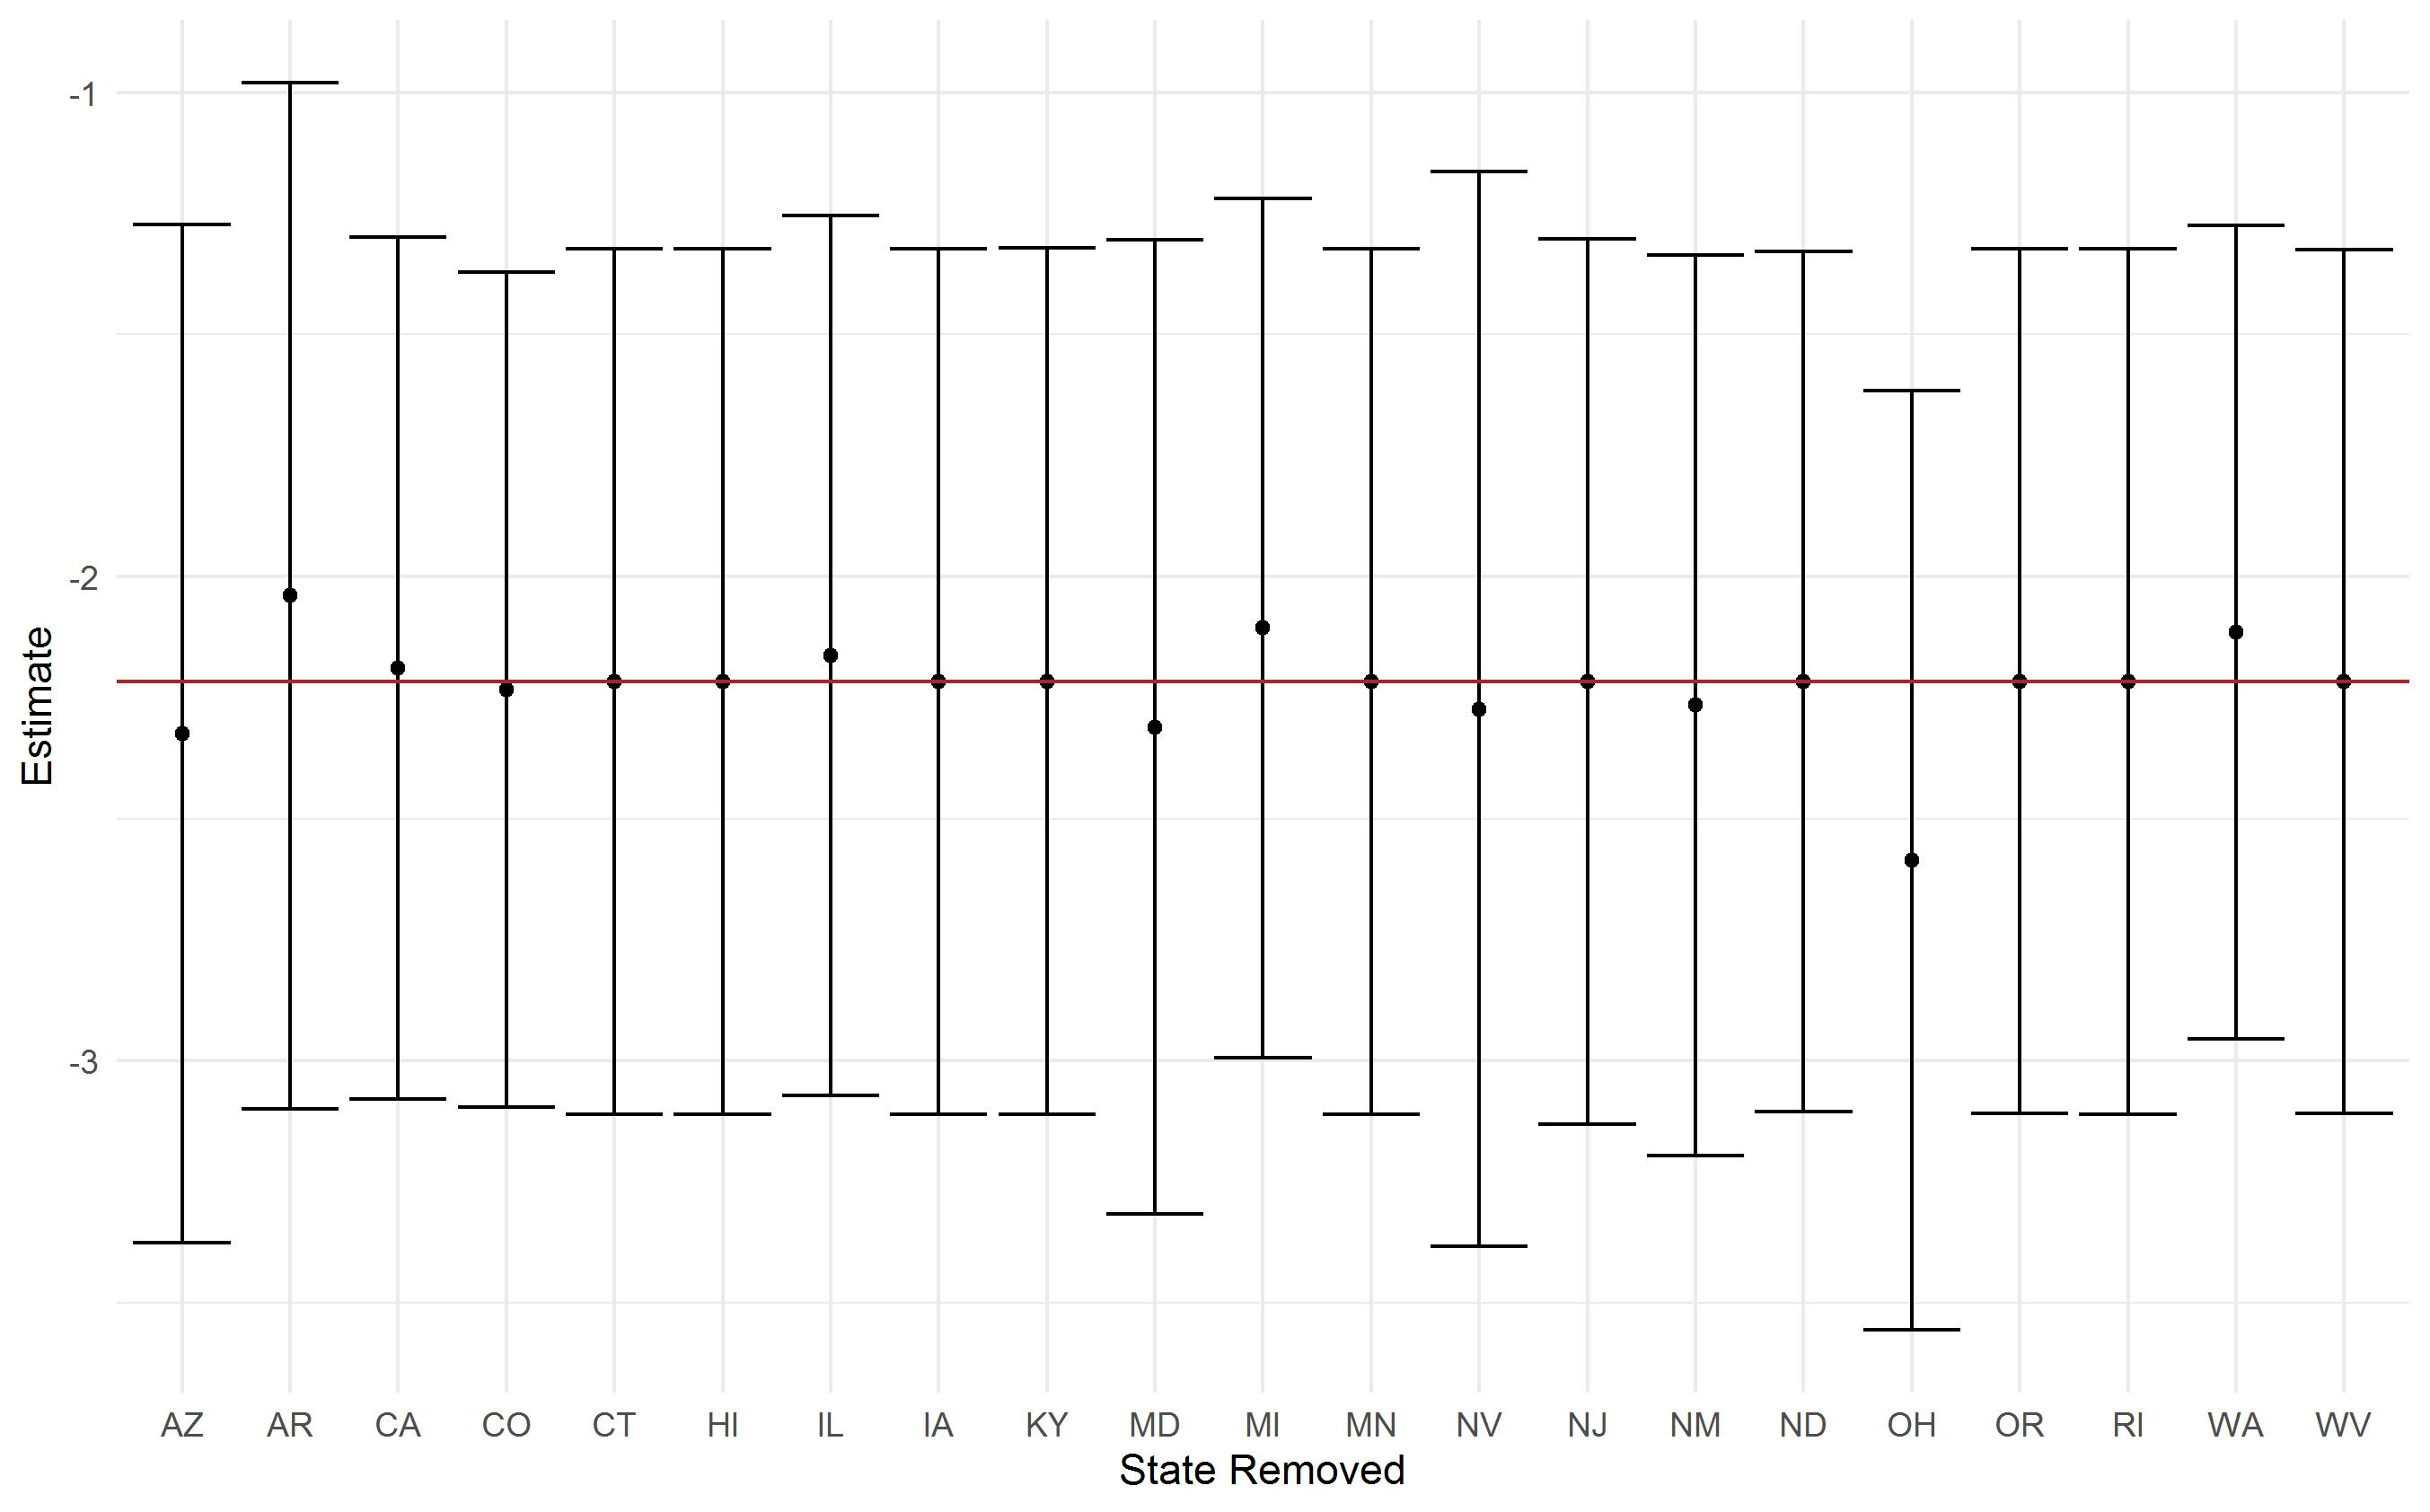
\includegraphics[scale=0.6]{images/loo-states-wt.jpeg}
    \caption{Leave-one-out state analysis: weighting estimator}
    \label{loostateswt}
\end{center}
\end{figure}

Figure \ref{loocovswt} presents the results for the weighting estimator for the leave-one-out covariate group analysis (the paper only presents the bias corrected estimator).

\begin{figure}[H]
\begin{center}
    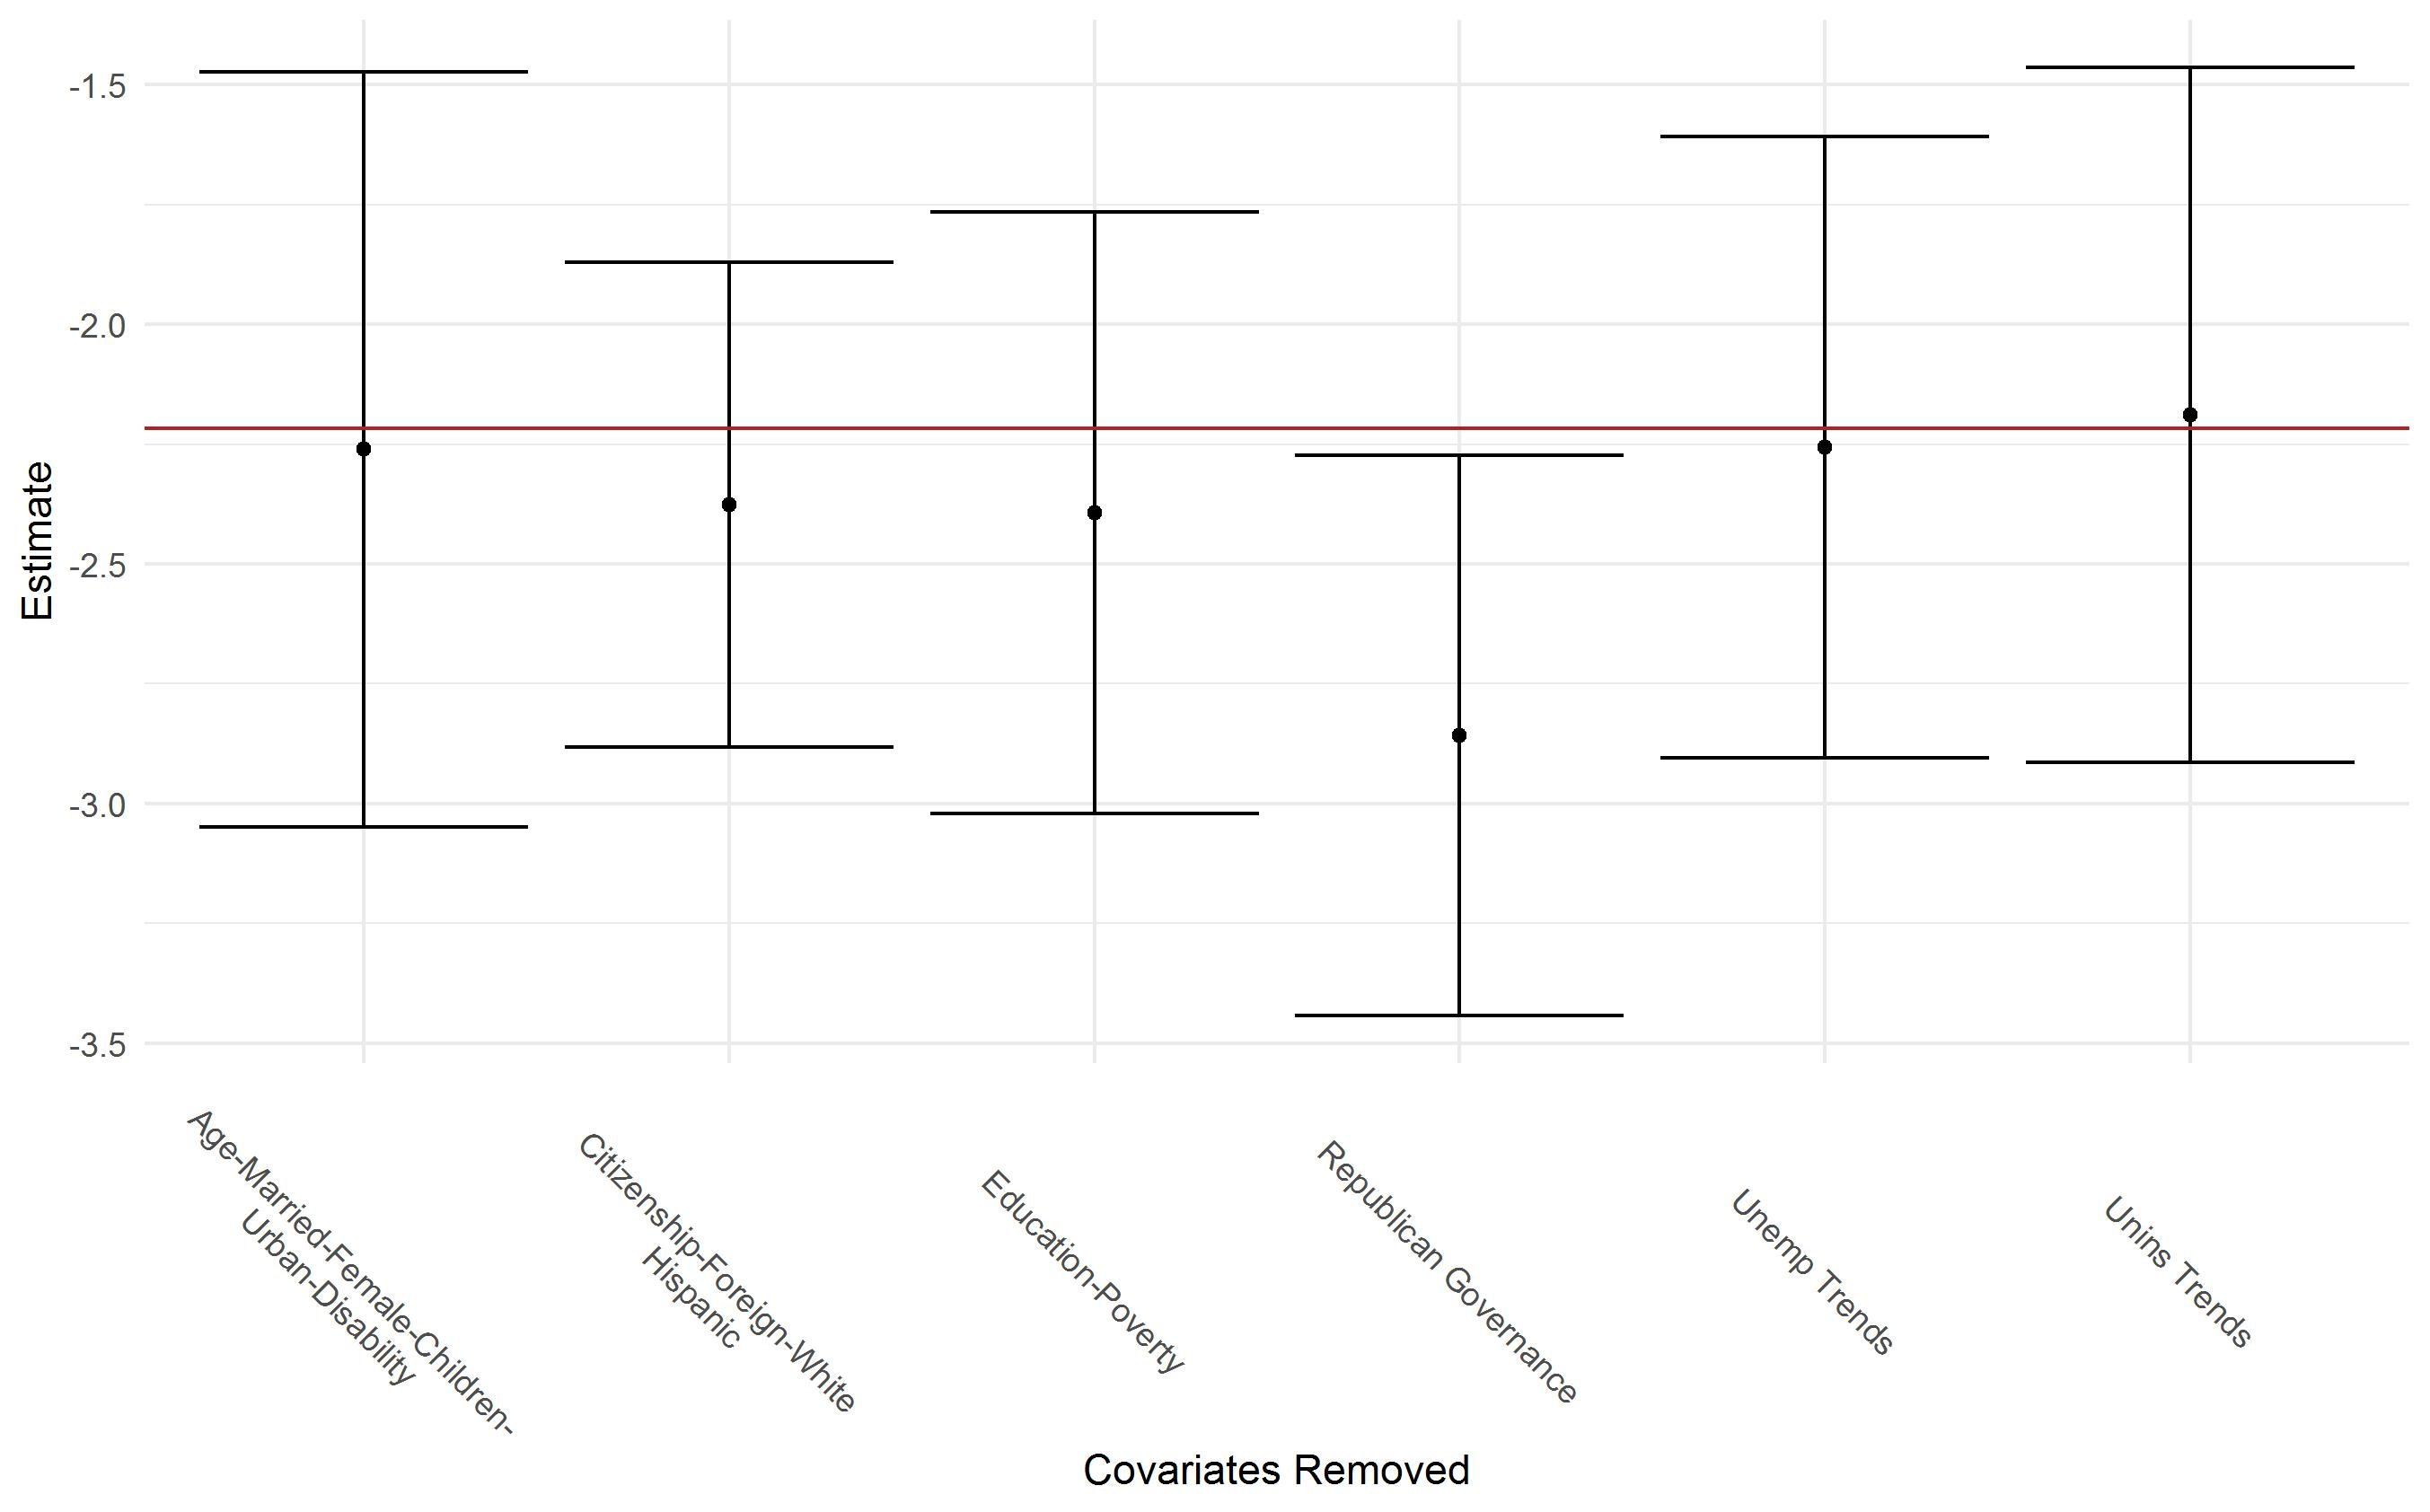
\includegraphics[scale=0.6]{images/loo-covariates-wgt.jpeg}
    \caption{Leave-one-out covariate group analysis: weighting estimator}
    \label{loocovswt}
\end{center}
\end{figure}

Figures \ref{loostatecovswt} and \ref{loostatecovsdr} below presents the associations between each covariate group and the estimated treatment effect when removing each non-expansion state one at a time. The red horizontal lines represent the estimated ETU for each set of states. The top figure presents results for the weighting estimator and the bottom figure for the bias-corrected estimator. We again see that Republican governance is negatively associated with the estimated treatment effect throughout.

\begin{figure}[H]
\begin{center}
    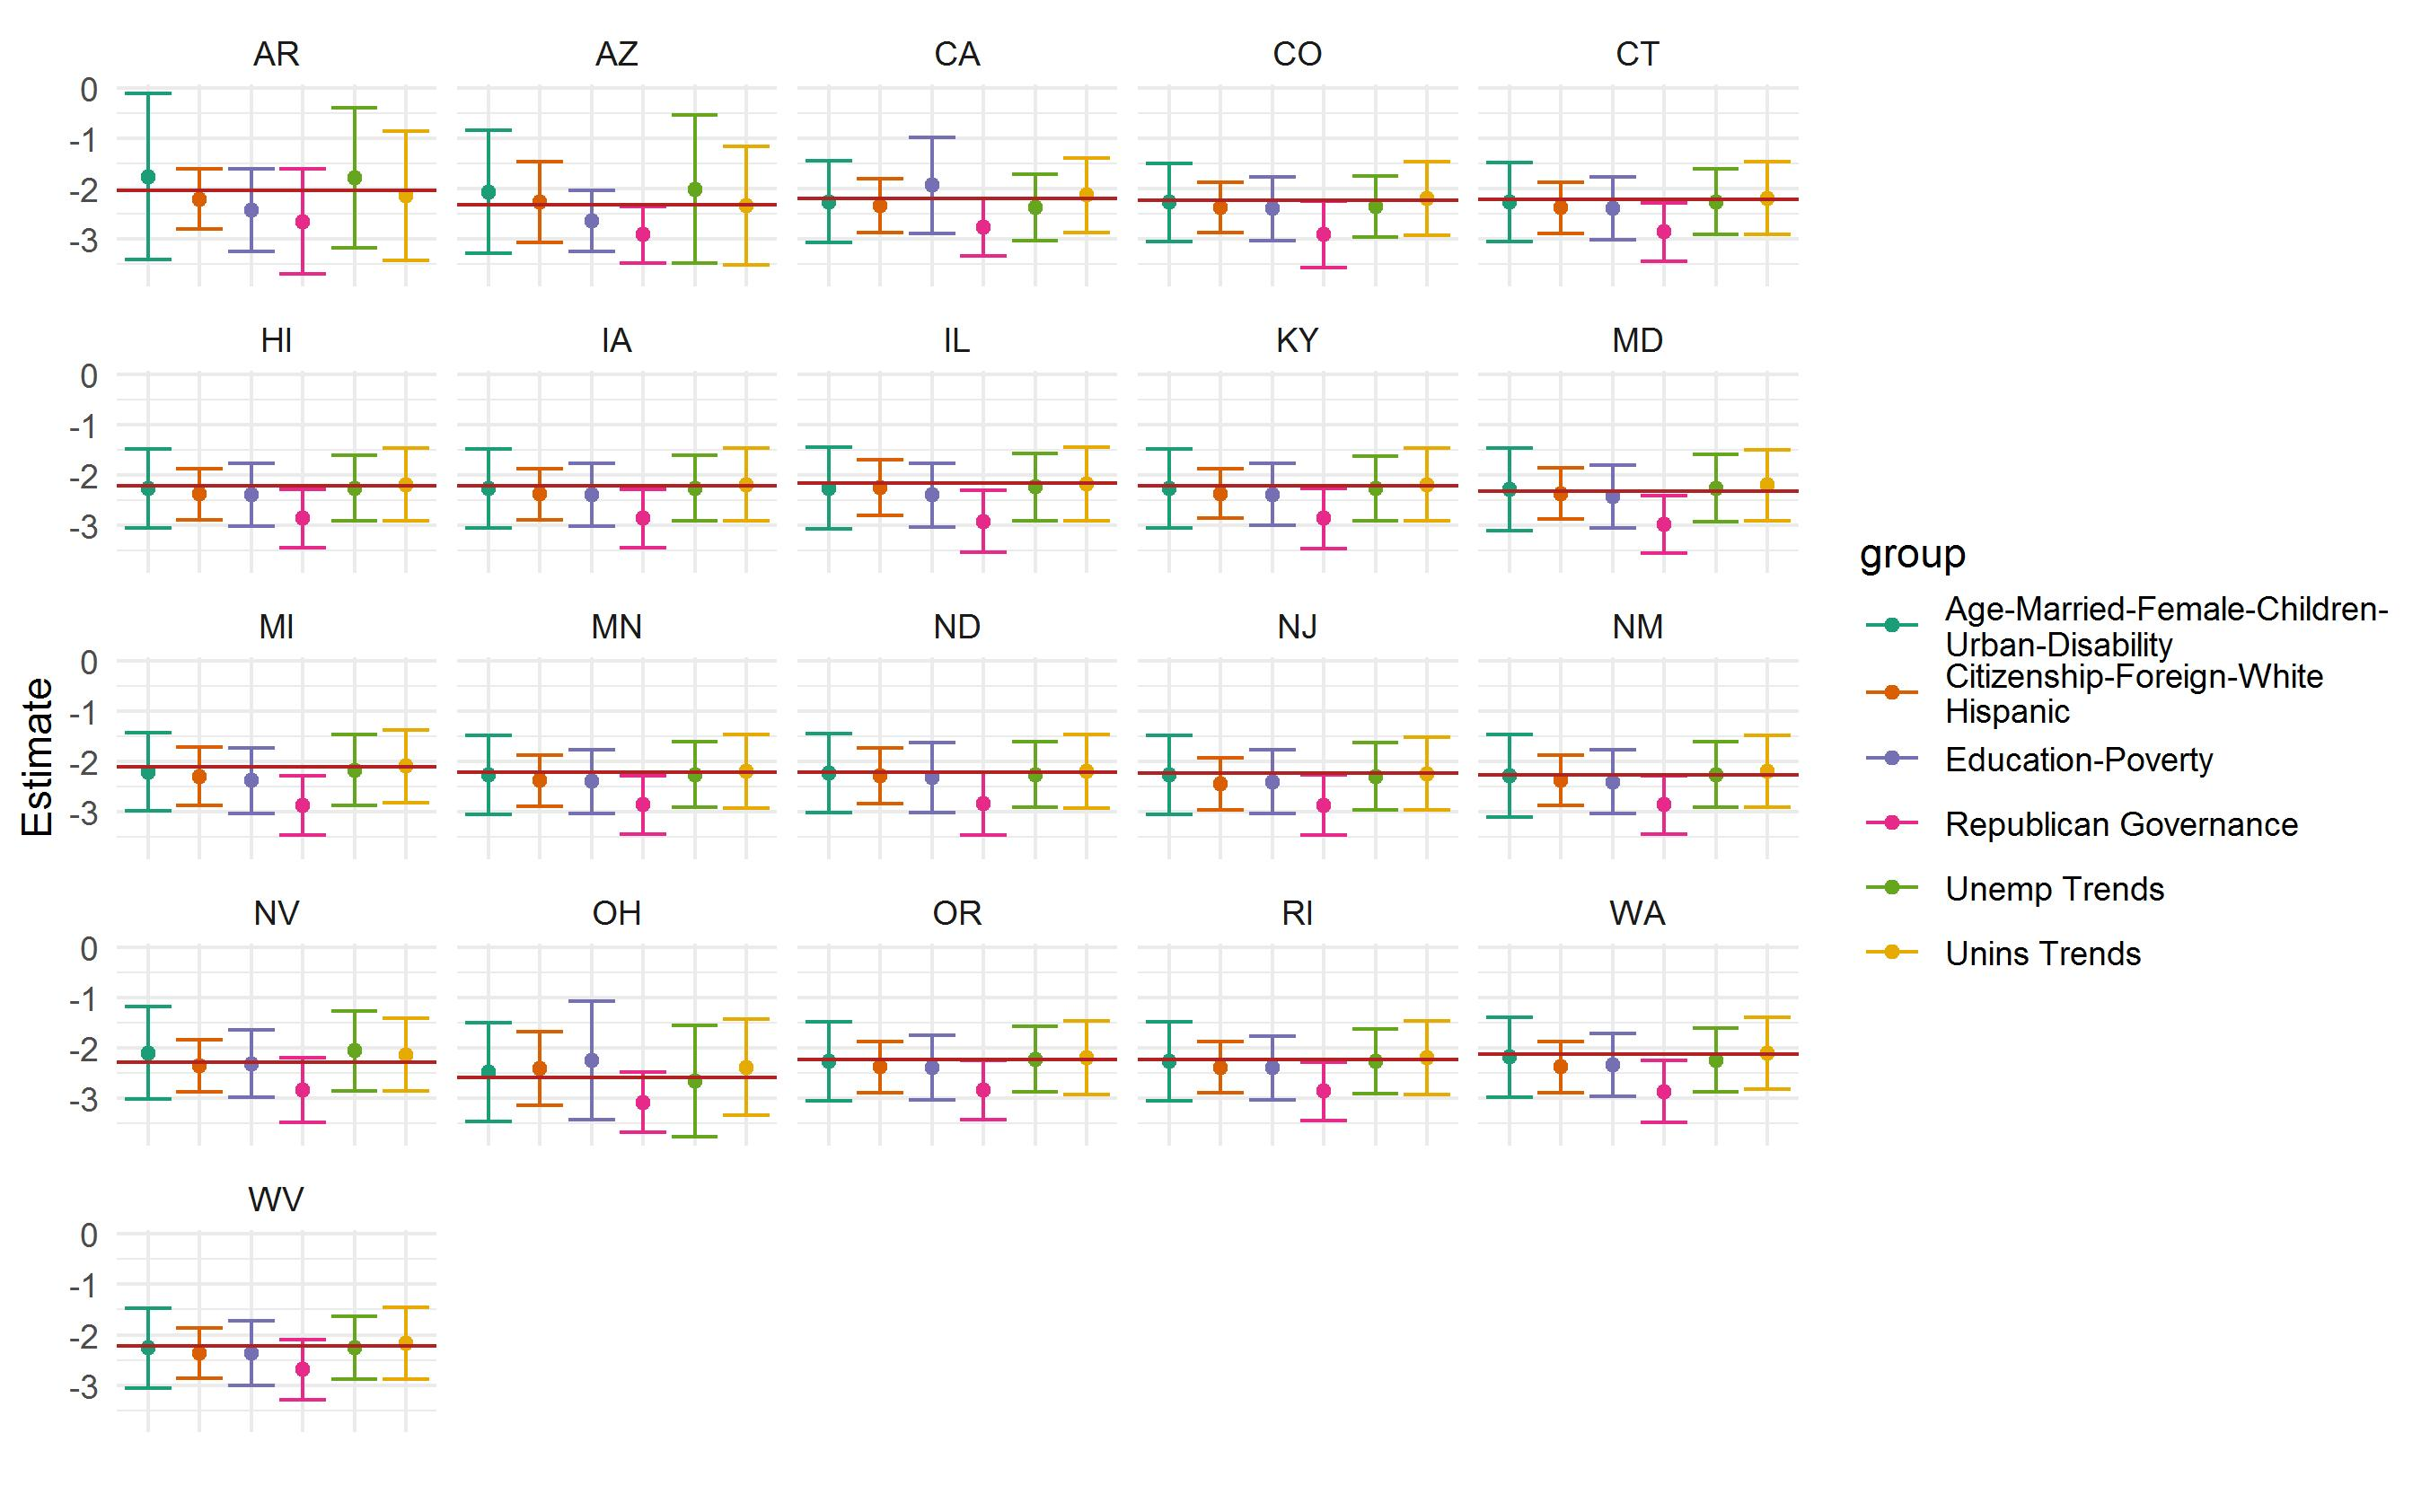
\includegraphics[scale=0.6]{images/loo-covs-state-all-wgt.jpeg}
    \caption{Leave-one-out states and covariate group analysis: weighting estimator}
    \label{loostatecovswt}
\end{center}
\end{figure}

\begin{figure}[H]
\begin{center}
    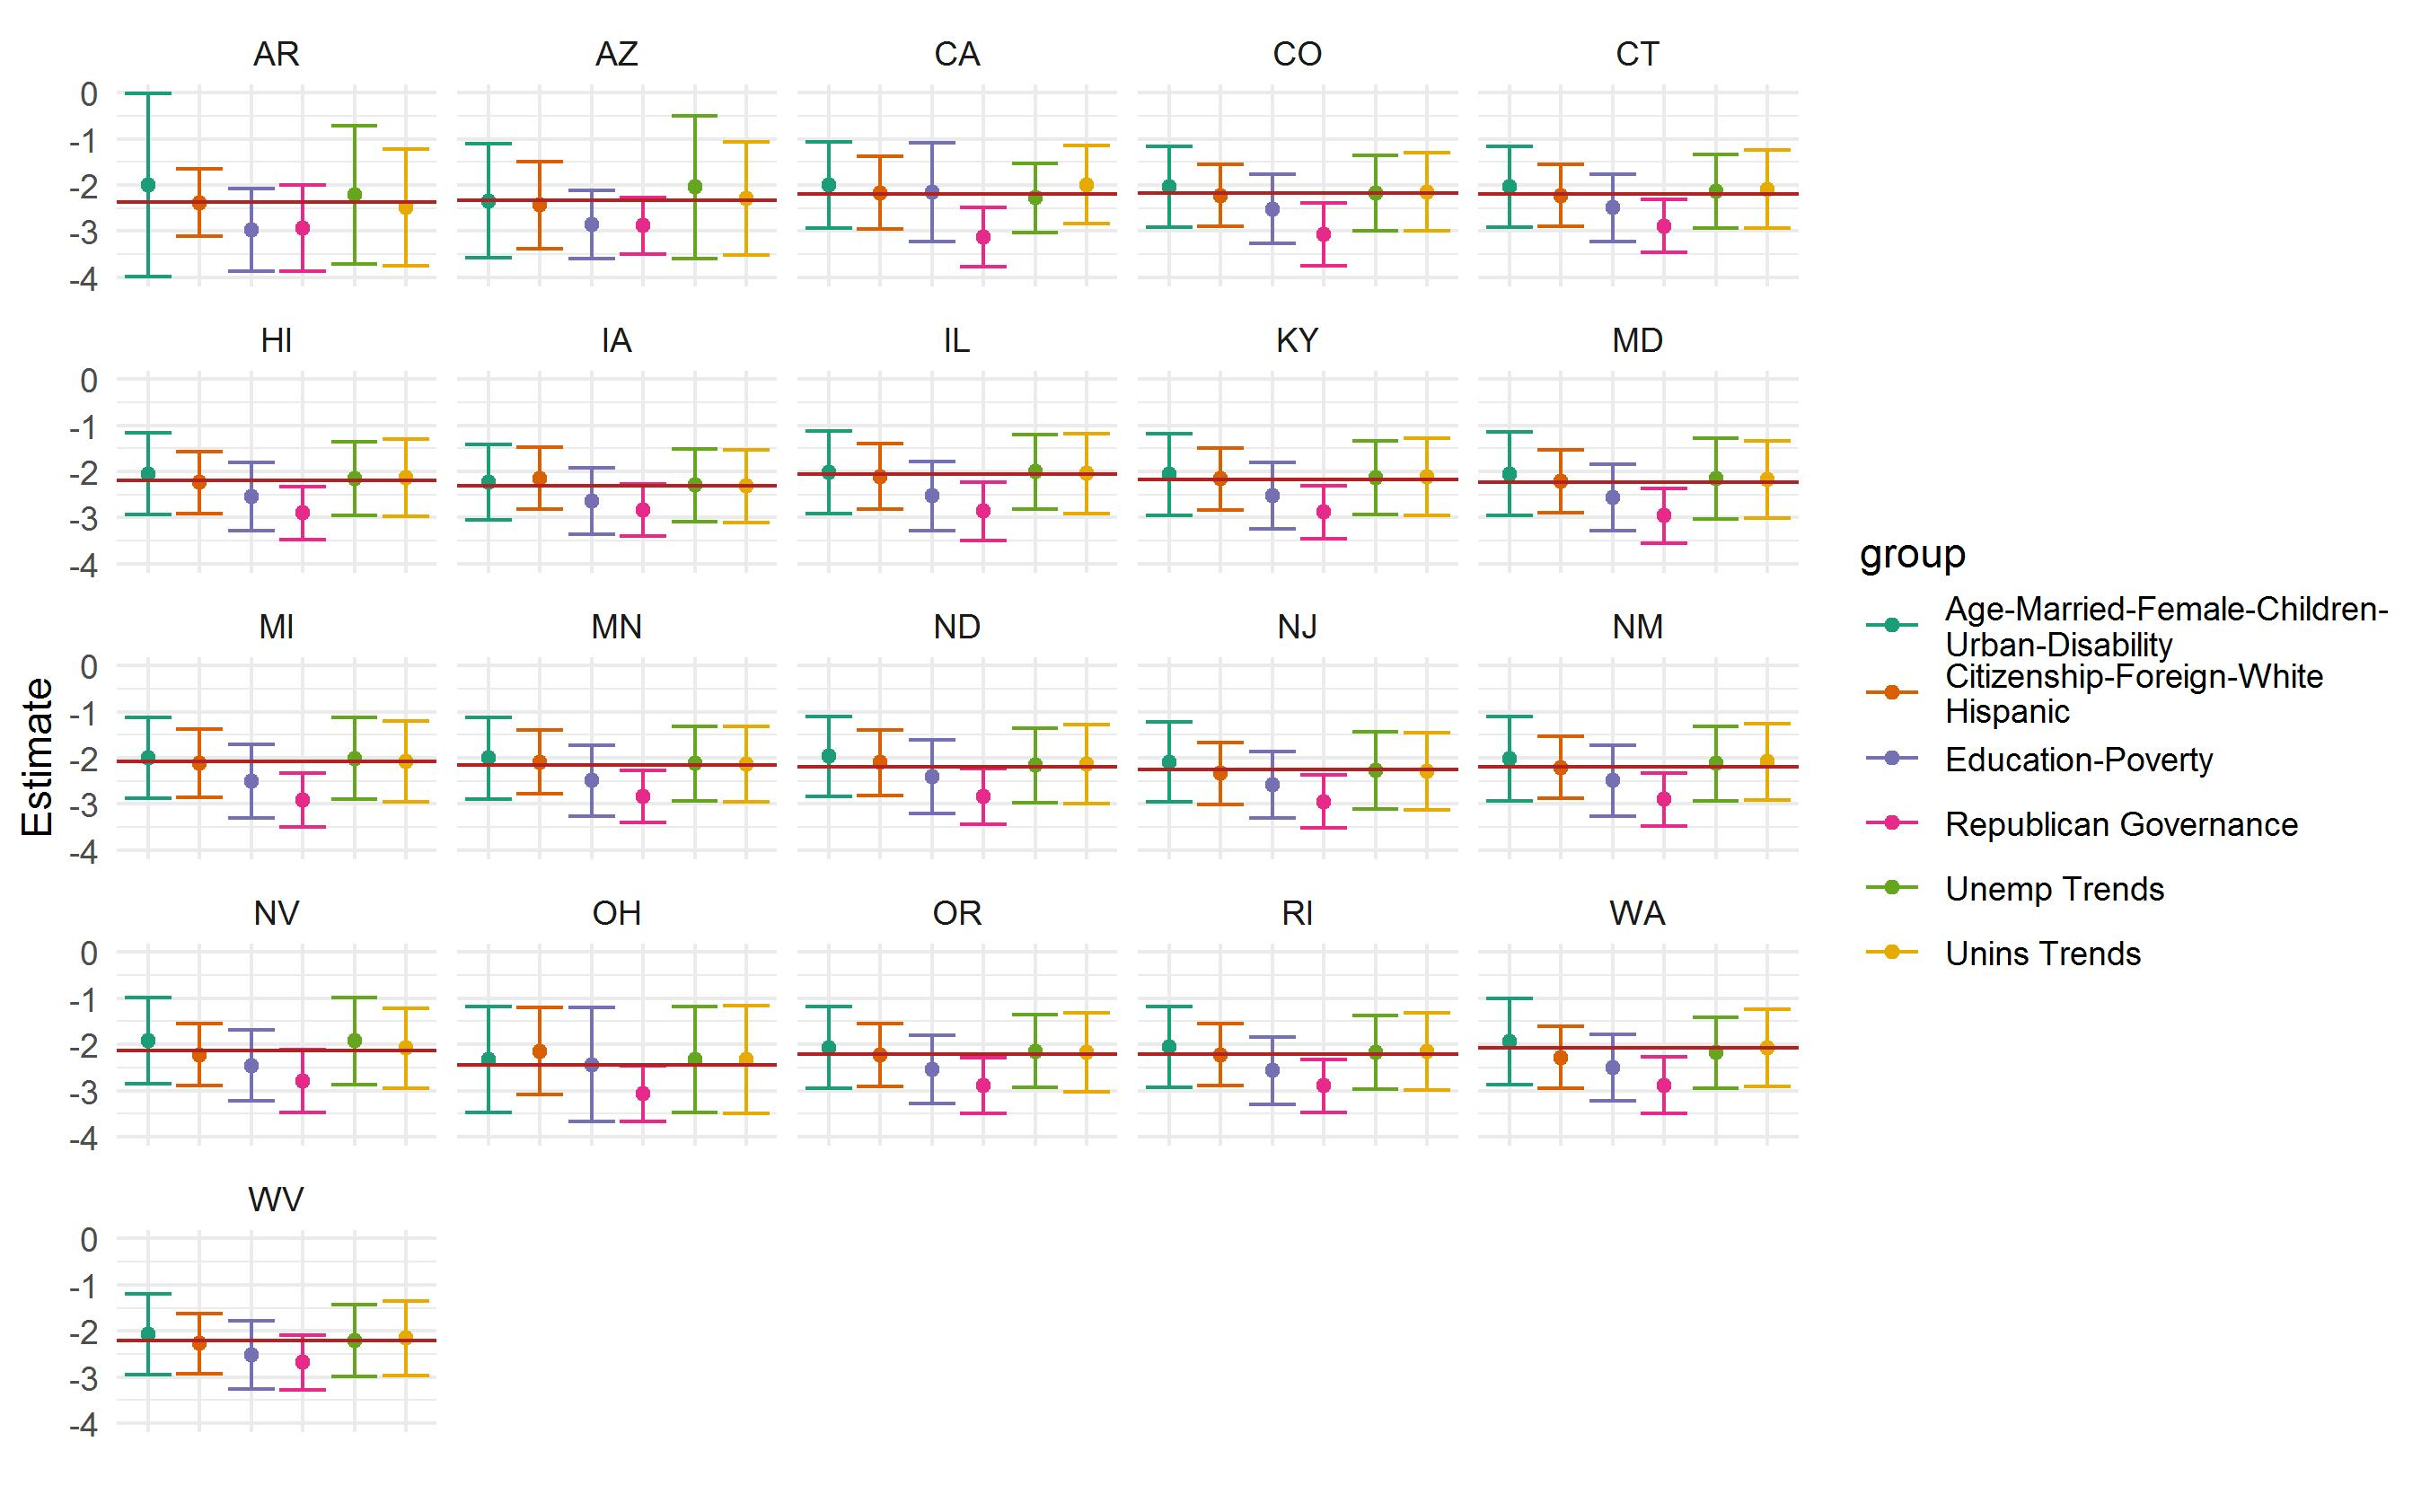
\includegraphics[scale=0.6]{images/loo-covs-state-all-dr.jpeg}
    \caption{Leave-one-out states and covariate group analysis: bias-corrected estimator}
    \label{loostatecovsdr}
\end{center}
\end{figure}

Figures \ref{eeloocovsswt} and \ref{eeloocovssdr} present the results of the leave-one-out covariate set when removing all early expansion states, for the weighting and the bias-corrected estimators, respectively.

\begin{figure}[H]
\begin{center}
    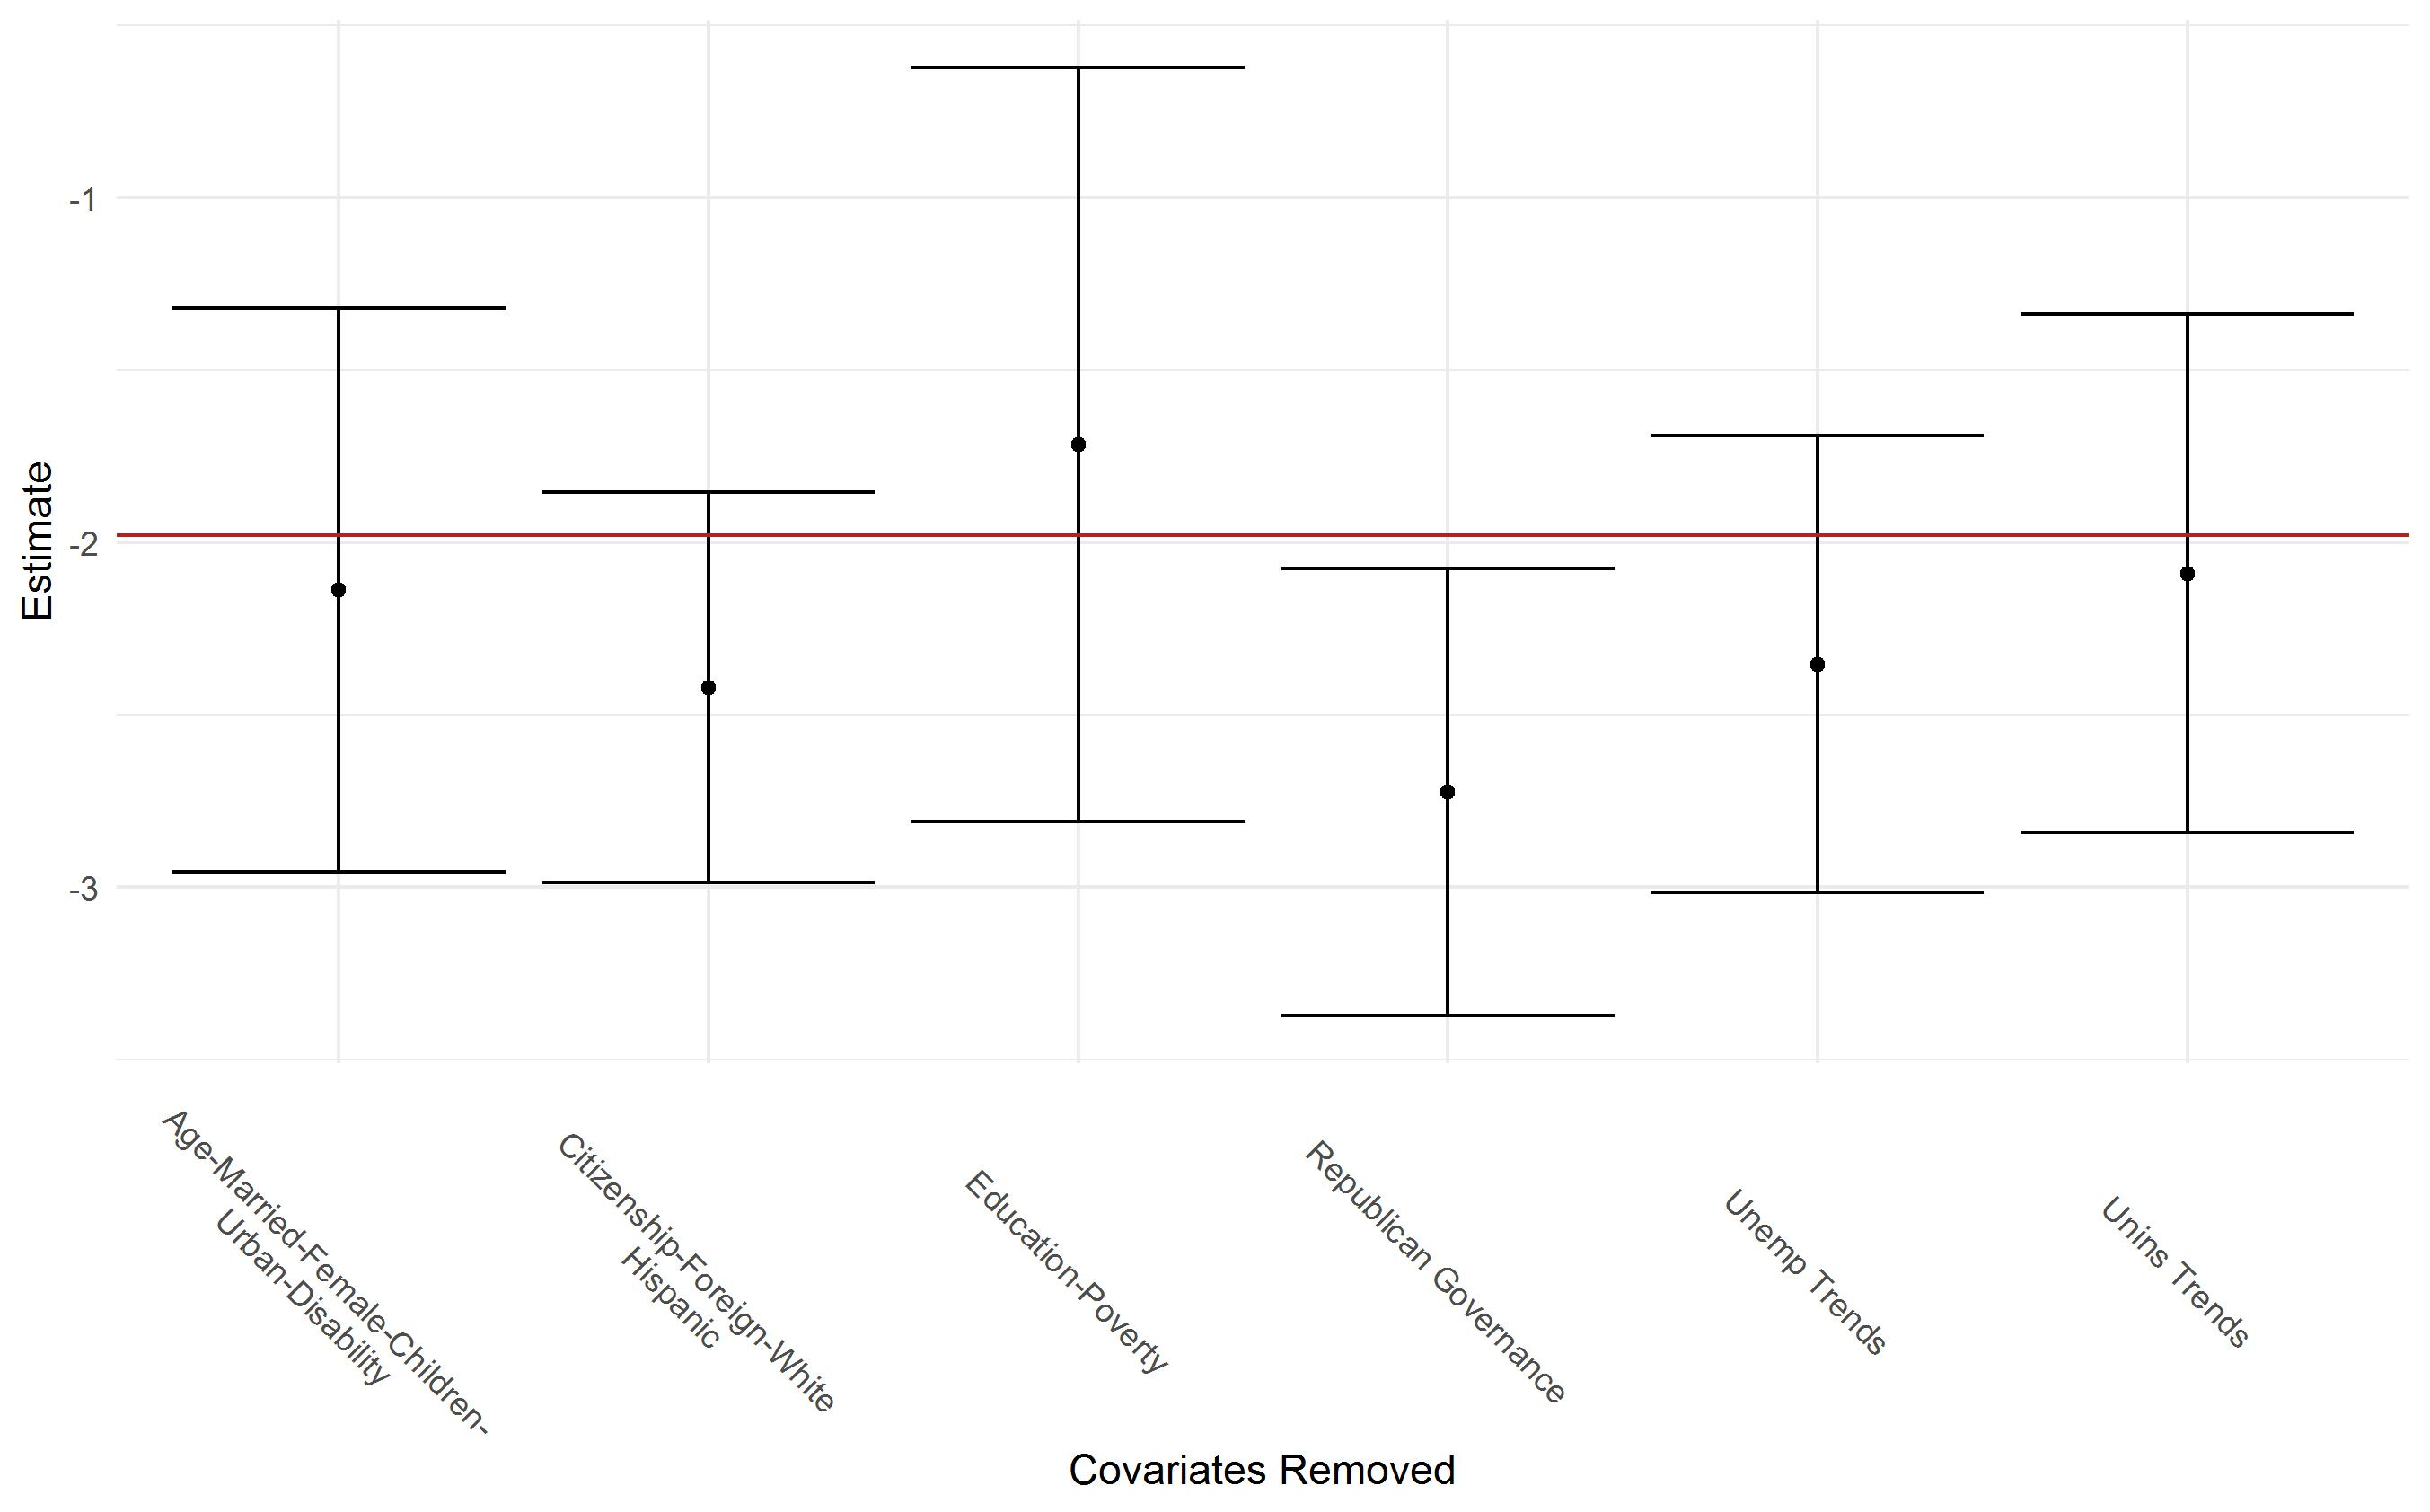
\includegraphics[scale=0.6]{images/loo-covariates-wgt-1.jpeg}
    \caption{Leave-one-out covariates: weighting estimator, early expansion removed}
    \label{eeloocovsswt}
\end{center}
\end{figure}

\begin{figure}[H]
\begin{center}
    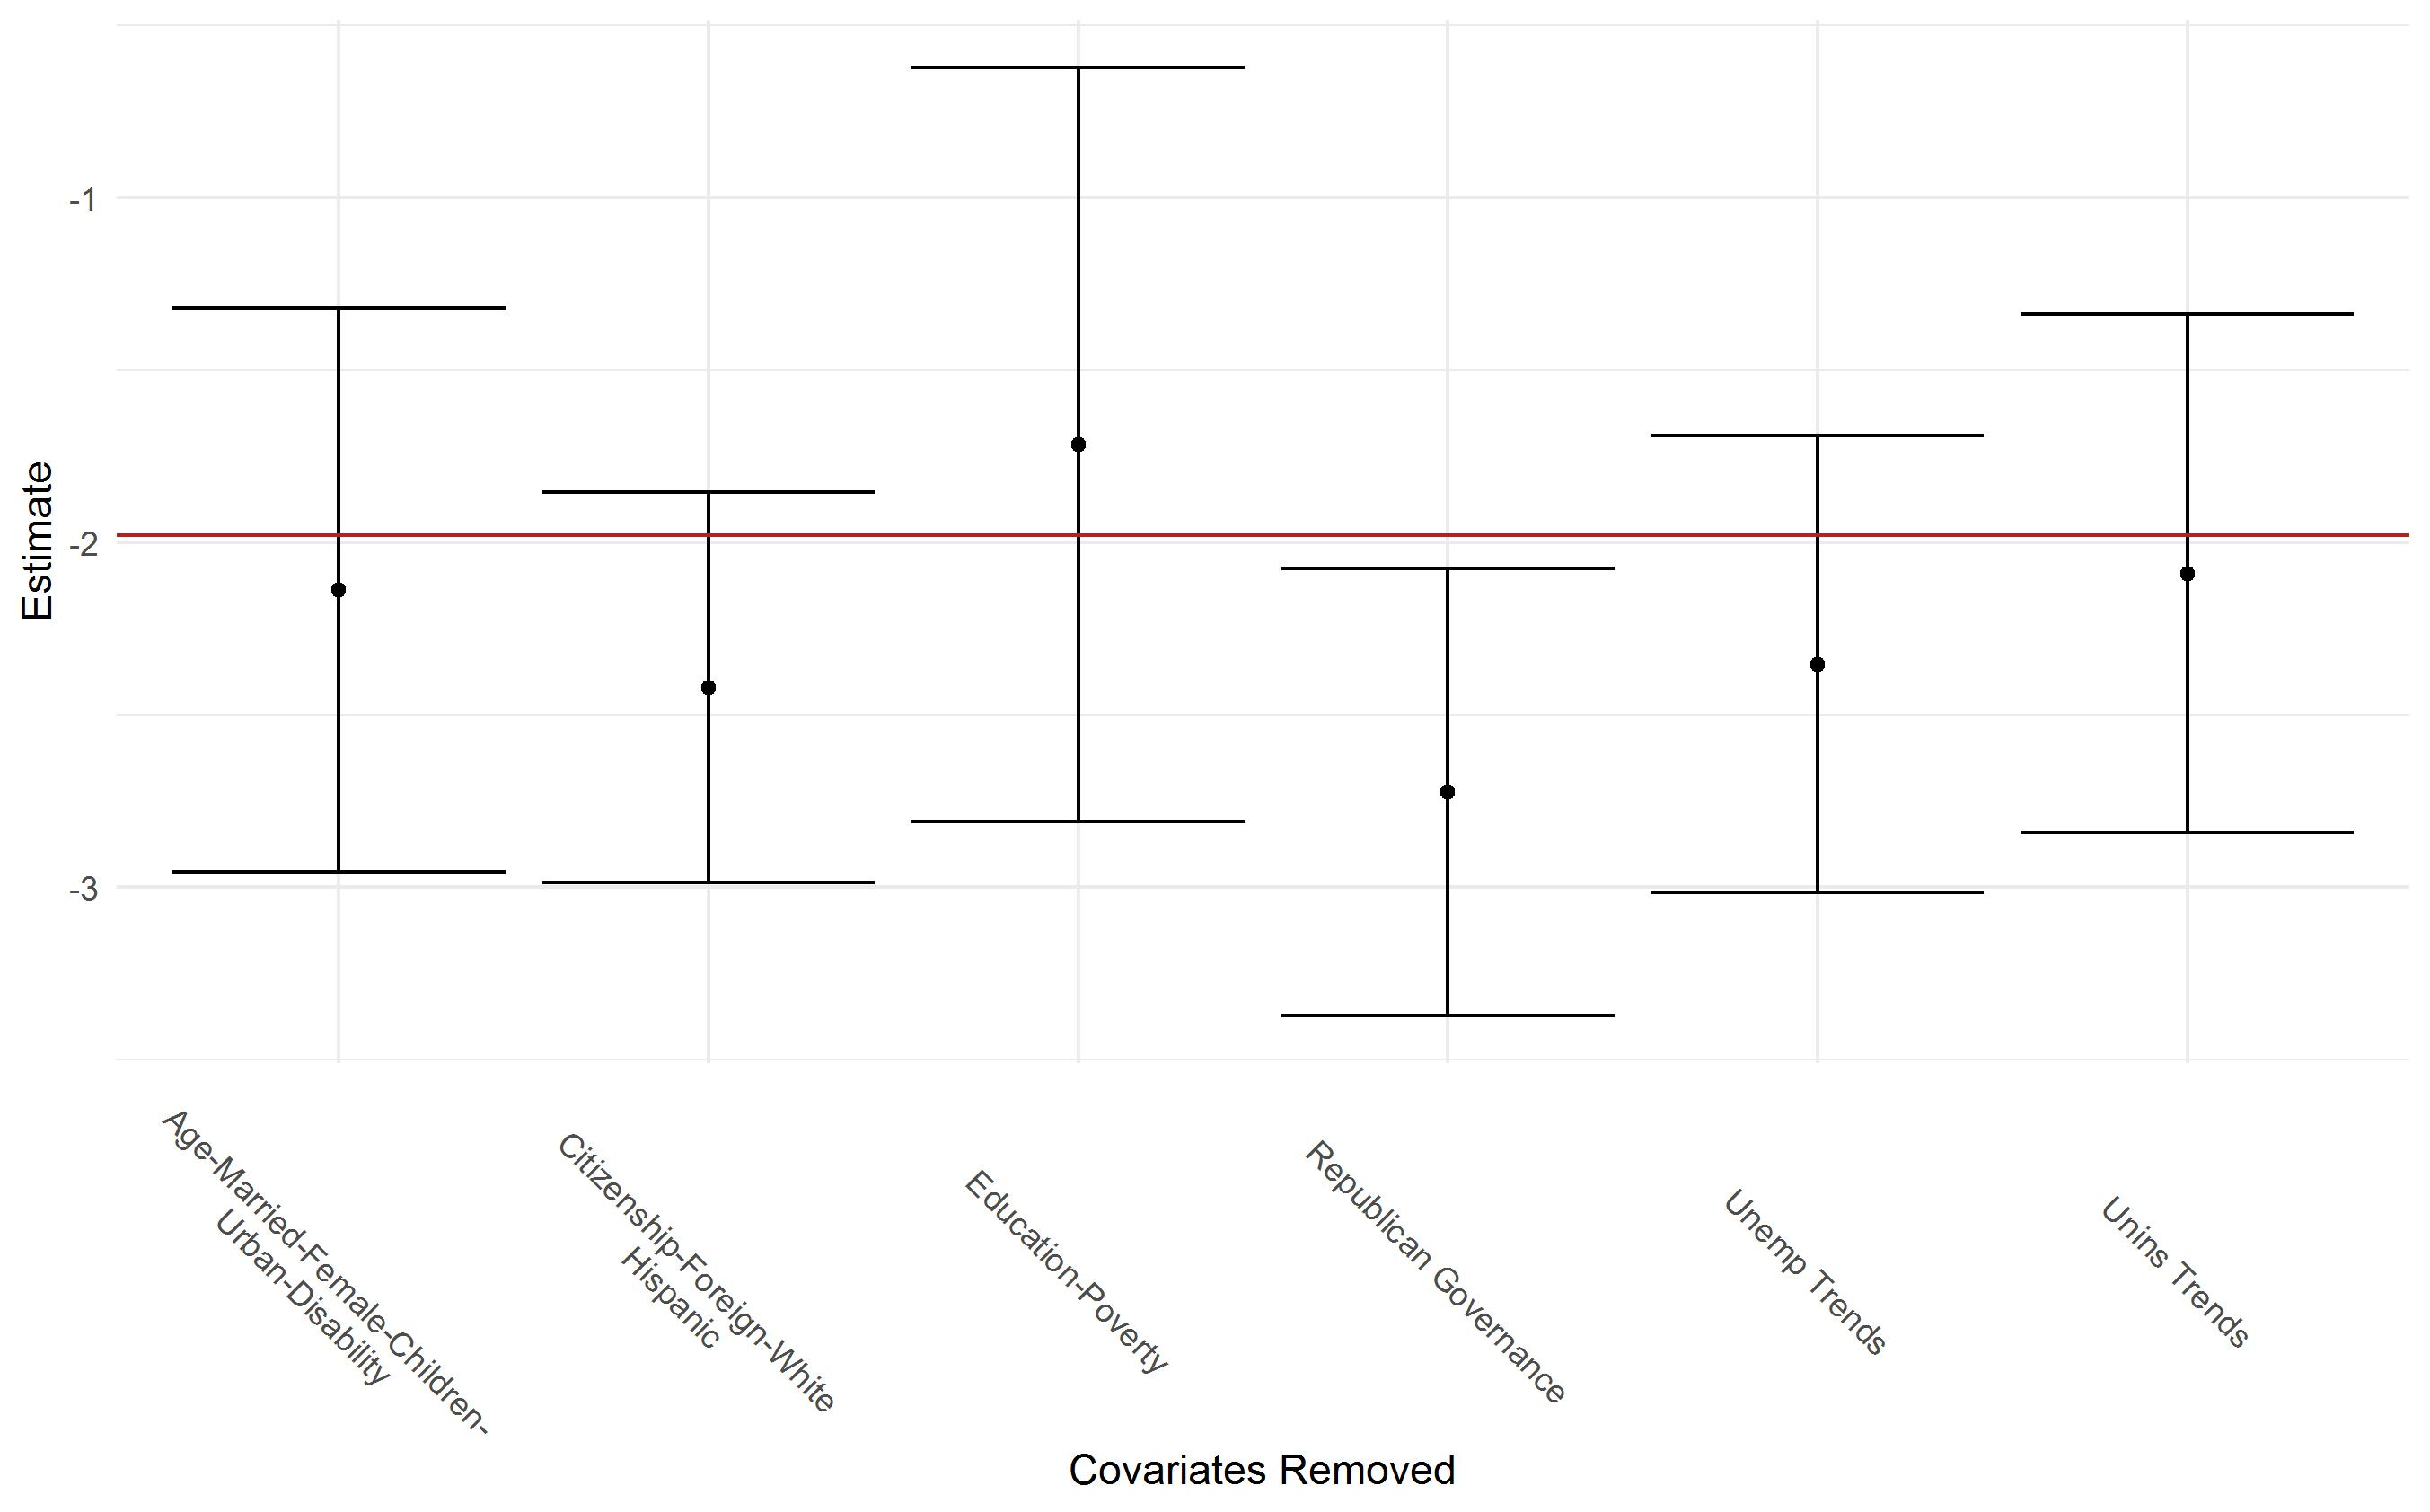
\includegraphics[scale=0.6]{images/loo-covariates-wgt-1.jpeg}
    \caption{Leave-one-out covariates: bias-corrected estimator, early expansion removed}
    \label{eeloocovssdr}
\end{center}
\end{figure}

\subsection{Appendix D: Additional OATE Results}

Figure \ref{oatestate} presents the associations between each covariate group and the estimated treatment effect when removing each non-expansion state one at a time. The red horizontal lines represent the estimated OATE for each set of states. We again see that Republican governance is negatively associated with the estimated treatment effect throughout.

\begin{figure}[H]
\begin{center}
    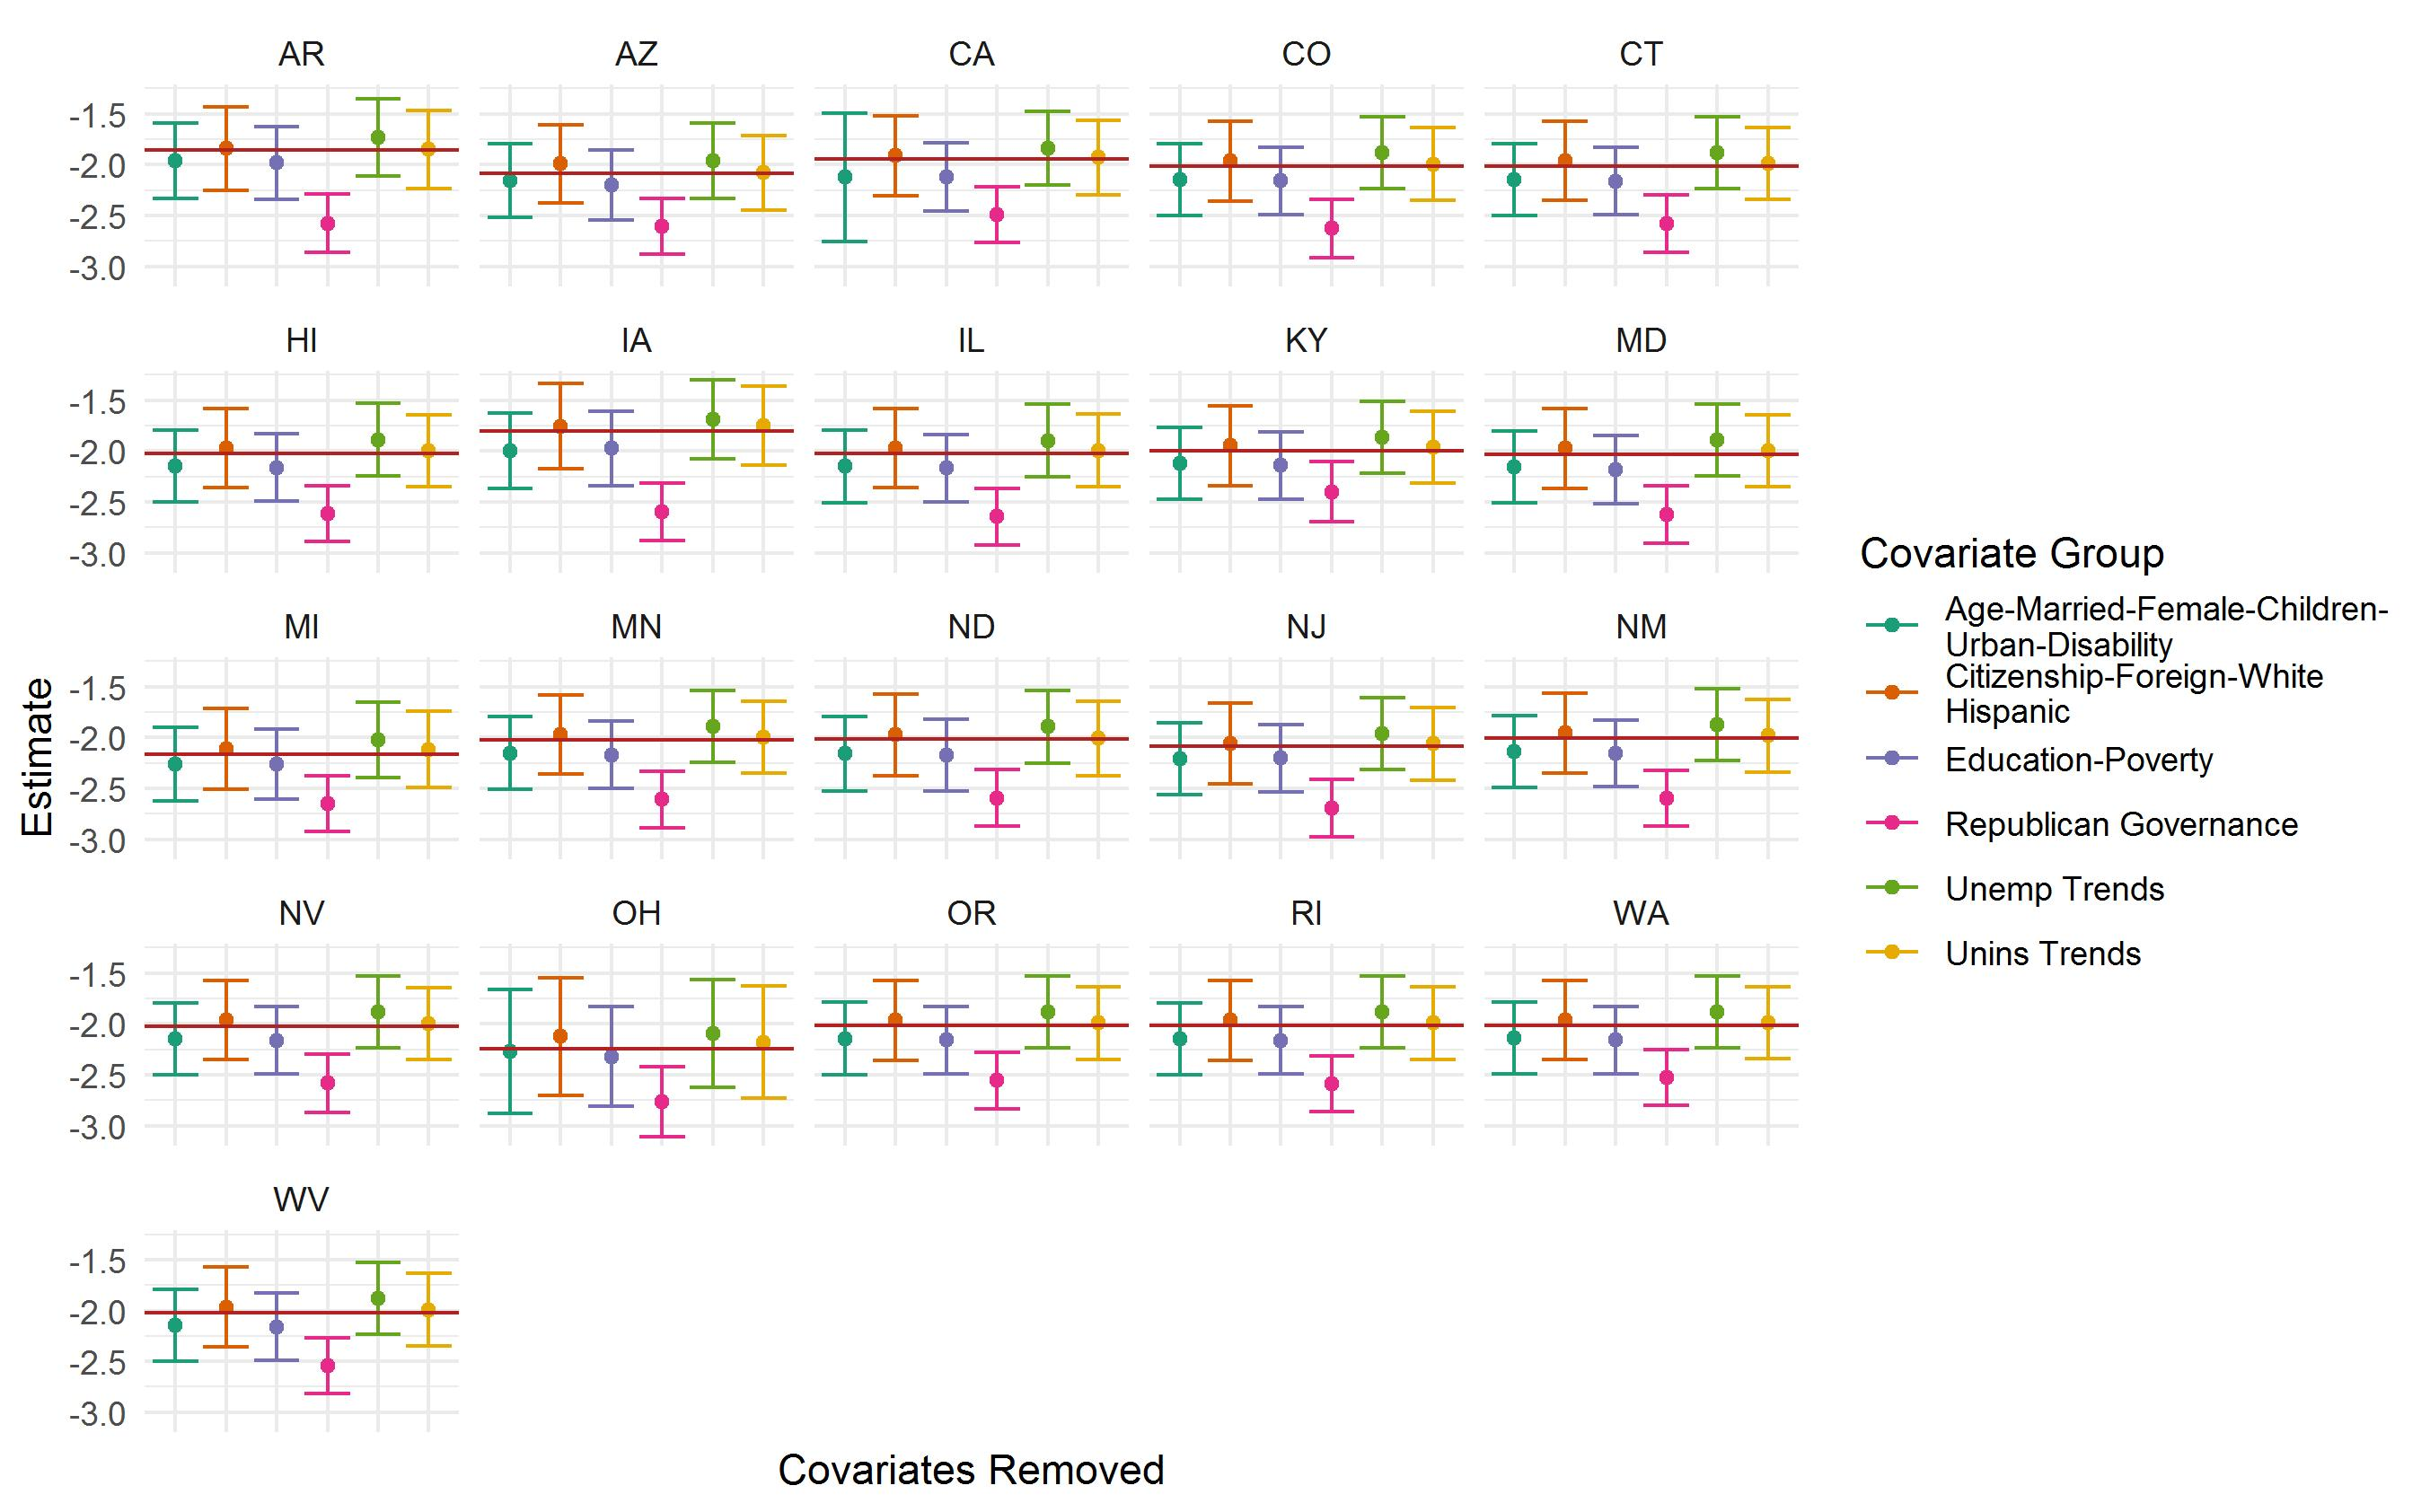
\includegraphics[scale=0.6]{images/oate-loo-covs-states.jpeg}
    \caption{OATE leave-one-out state and covariate group analysis}
    \label{oatestate}
\end{center}
\end{figure}

\subsection{Appendix E: Covariate Correlations}

We briefly present additional information about the correlations between our covariates. Given the relatively high-dimensionality of this problem, the fact that many of our covariates are highly correlated made balancing our covariates more tractable. For example, the pairwise correlations between all of the denominator variables are close to 1. Excluding these counts, we briefly consider the remaining 465 pairwise correlations.

We find the minimum correlation of 0.45, a maximum of approximately 1, first quartile of 0.78, third quartile of 0.95, median of 0.92 and mean of 0.87. The top three largest pairwise correlations were between the pre-treatment number of uninsured. The lowest pairwise correlations were between the Republican governance indicators and the number of hispanic and foreign born residents. The lowest pairwise correlation not involving the governance indicators was between the number of foreign born and the number of people with disabilities (0.53). 

We now present the (first quartile, median, third quartile) within each covariate group that we used for the the leave-one-out covariate group analysis. Among the first group (age, children, number of households, married, female, urban, disability) we find (0.95, 0.98, 0.99). For the second group (citizenship, foreign born, white, hispanic) we find (0.87, 0.92, 0.96). For the third group (education, income-to-poverty group, student) we find (0.87, 0.93, 0.96); the fourth group (Republican governance) we find (0.88, 0.90, 0.91) the fifth group (unemployed, labor force) we find (0.95, 0.96, 1); and lastly the sixth group (uninsured, adult population) we find (1, 1, 1).

\end{document}






